\documentclass[hyperref=colorlinks]{beamer}
\mode<presentation>
\usetheme{iclpt}
\setbeamertemplate{navigation symbols}{}
\setbeamertemplate{headline}{
\begin{beamercolorbox}[leftskip=.2cm,rightskip=.2cm,topskip=.2cm,ht=1.1cm,dp=0.1cm,wd=\textwidth]{institute in head/foot}
  
\includegraphics[height=1cm]{icl.pdf}
  \hfill
  
\includegraphics[height=1cm]{../Pics/CMS-Color.pdf}
\end{beamercolorbox}
}
\setbeamertemplate{footline}{
\begin{beamercolorbox}[ht=.55cm,dp=0.4cm,wd=\textwidth,leftskip=.3cm]{author in head/foot}%
  \begin{minipage}[c]{5cm}%
    \usebeamerfont{author in head/foot}
    \insertshortauthor 
    \insertshorttitle
    \end{minipage}\hfill%
  \insertframenumber{} / \pageref{lastframe}
  \hfill
  \begin{minipage}{6cm}
    \hfill
  \end{minipage}
\end{beamercolorbox}%
}

\usepackage{color}
\usepackage{tabularx,colortbl}
\usepackage{graphicx}
\usepackage{pdfpages}
\usepackage{feynmp}
\usepackage{multirow}
\DeclareGraphicsRule{*}{mps}{*}{}

\title{\vspace{-0.2cm} VBF Higgs to Invisible Trigger Efficiencies}
%\subtitle{This result: HIG-15-012 \\ Contributing analyses: HIG-13-030, HIG-14-038, EXO-12-055}
\author[P. Dunne]{P. Dunne A. Magnan for H$\rightarrow$inv. group}
\titlegraphic{
  \vspace{-0.7cm}
  %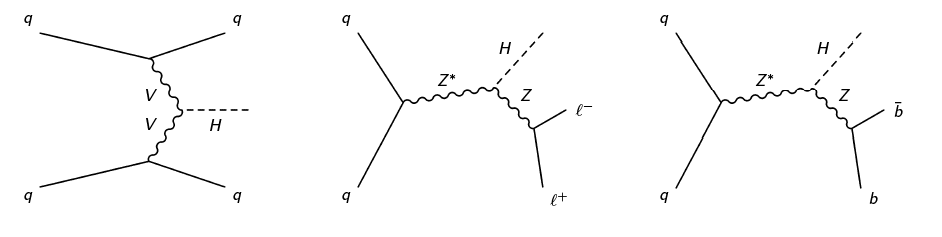
\includegraphics[width=\textwidth]{TalkPics/invcomb021213/feyndiags}
%% \begin{fmfgraph*}(100,70)
%%         \fmfleft{i1,i2}
%%         \fmfright{o1,o2,o3}
%%         \fmf{fermion}{i1,v1,o1}
%%         \fmf{fermion}{i2,v2,o3}
%%         \fmf{phantom,tension=4/5}{v1,v2}
%%         \fmffreeze
%%         \fmf{photon,label=$W,,Z$}{v1,v3}
%%         \fmf{photon,label=$W,,Z$}{v2,v3}
%%         \fmf{dashes}{v3,o2}
%%         \fmflabel{$q$}{i1}
%%         \fmflabel{$q$}{i2}
%%         \fmflabel{$q$}{o1}
%%         \fmflabel{$q$}{o3}
%%         \fmflabel{$H$}{o2}
%%       \end{fmfgraph*}
}
\date{}
\begin{document}
\begin{fmffile}{hexotrig261015feyndiags}

%TITLE PAGE
\section{Title}
\begin{frame}
  \titlepage
  
\end{frame}

%OUTLINE
\begin{frame}
  \frametitle{Reminder and outline}
  \scriptsize
  \begin{block}{}
    \begin{itemize}
      \item We have previously seen slow trigger turn ons in met (300 GeV 95\% efficiency) and jet 2 pt (80 GeV 95\% efficiency)
      \item We have looked at jet pt turn on in a separate trigger path: HLT\_PFHT750\_4JetPt50
      \item Behaviour seen there motivates studies of L1 MET turn on and calo jet prefilter
      \item Will go through studies then show again plots to be presented for DPS approval at Higgs tomorrow
    \end{itemize}
  \end{block}
\end{frame}

\begin{frame}
  \frametitle{Turn on in jet only trigger}
  \scriptsize
  \vspace{-.2cm}
  \begin{block}{}
    \begin{itemize}
    \item Have pass/fail information for HLT\_PFHT750\_4JetPt50
    \item Denominator: SingleMuon events with HT$>$1200 GeV
    \item[-] 1200 is the 90\% efficiency point
    \item Curve looks good, over 90\% efficient by 60 GeV
    \end{itemize}
  \end{block}
  \centering
  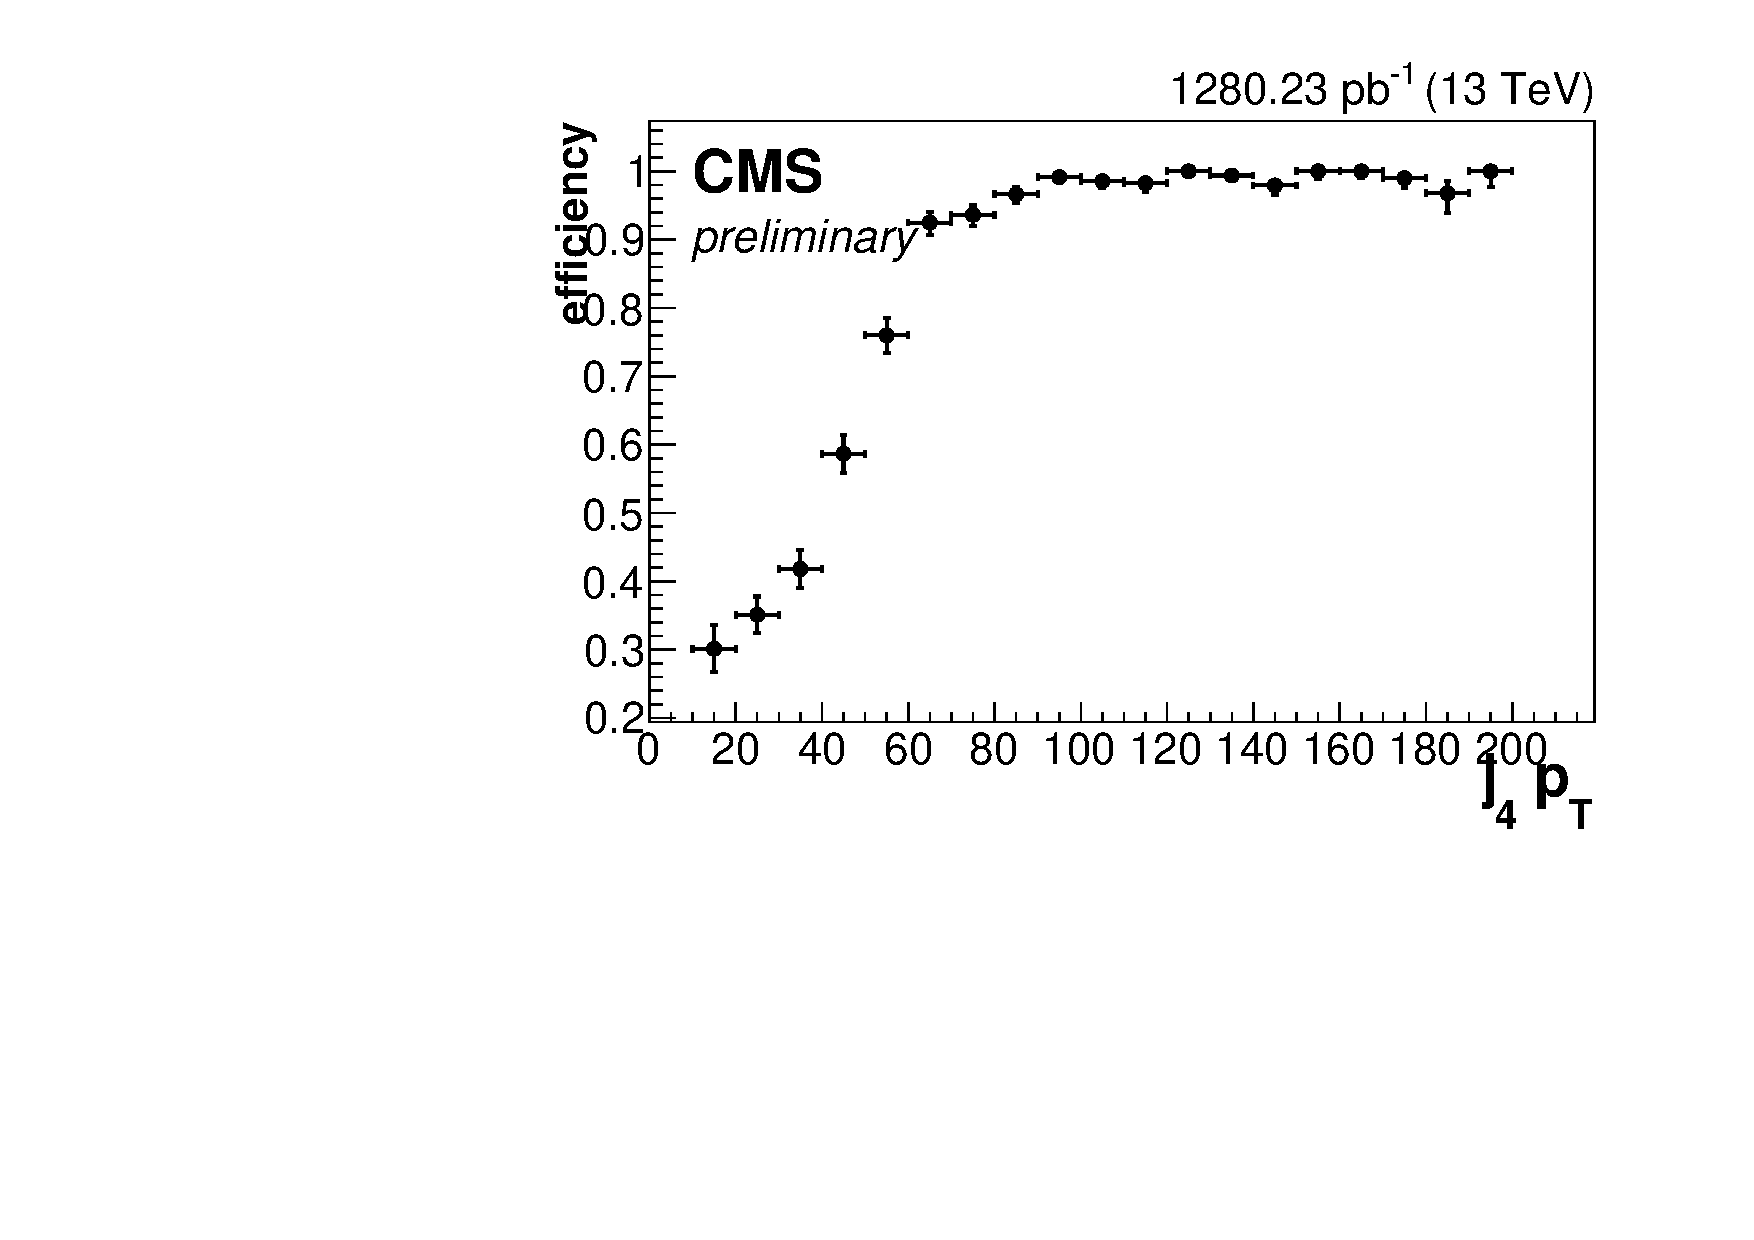
\includegraphics[width=.5\textwidth]{TalkPics/trigeffandpheno041115/nunu_jet4_pt.pdf}
\end{frame}

\begin{frame}
  \frametitle{Implications for our trigger}
  \scriptsize
  \begin{block}{}
    \begin{itemize}
    \item As 4JetPt50 trigger behaves well examine differences from our trigger:
    \item 4JetPt50 has no L1ETM requirement:
    \item[-] Study L1ETM turn on
    \item[-] Shown in next few slides
    \item 4JetPt50 has no calo jet pt prefilter:
    \item[-] According to \href{https://indico.cern.ch/event/456813/contribution/0/attachments/1178012/1704076/15-10-28_News_PPD.pdf}{these slides} wrong JEC was used in HLT during Run2015      
    \item[-] We only have trigger jet information in events that pass the trigger
    \item[-] Study HLT Calo vs offline PF jet response
    \item[-] Shown later
      \end{itemize}
  \end{block}
\end{frame}

\begin{frame}
  \frametitle{L1ETM60 Efficiency: Inclusive}
  \scriptsize
  \begin{block}{}
    \begin{itemize}
    \item Measure L1 ETM turn on
    \item Trigger: L1ETM60
    \item Denominator: SingleMuon events passing HLT\_IsoMu20
    \item 95\% efficient by 200 GeV 
    \end{itemize}
  \end{block}
  \centering
  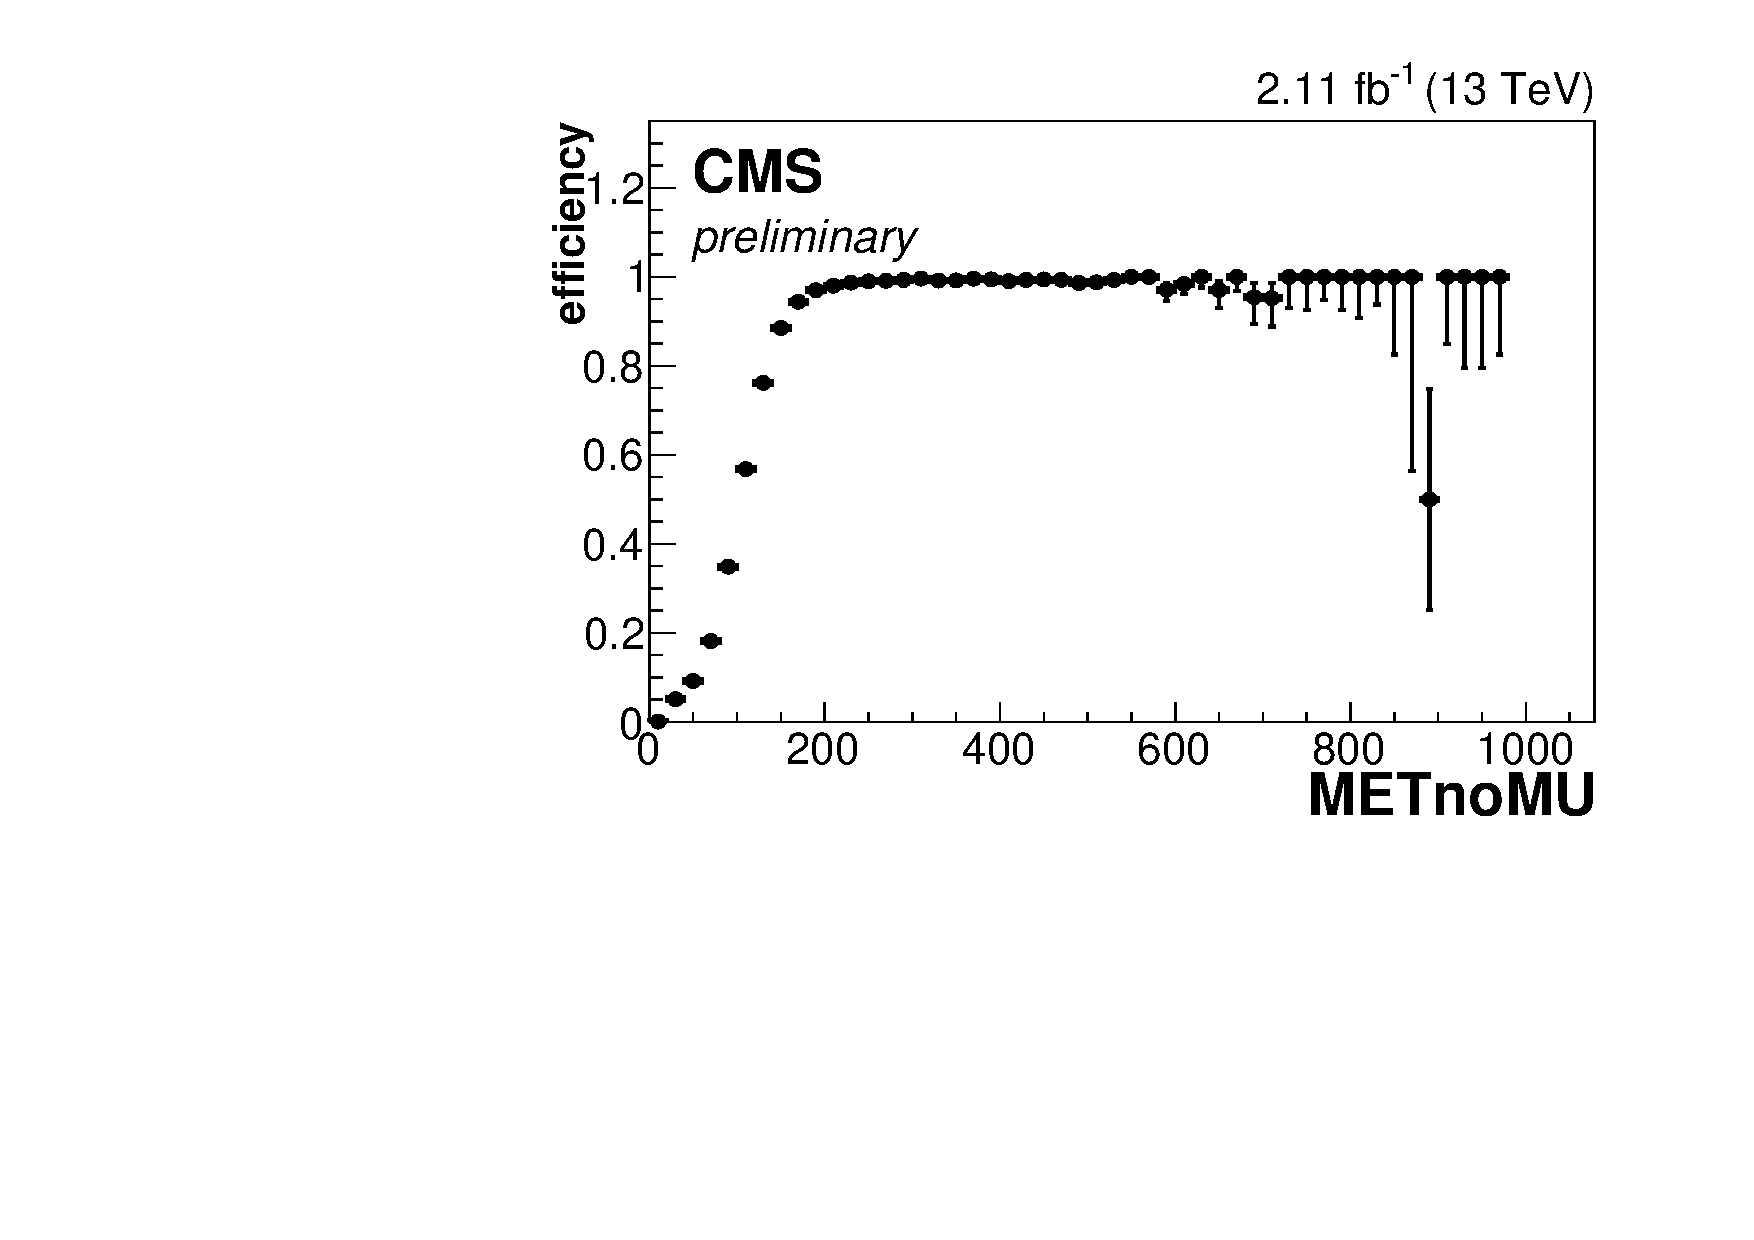
\includegraphics[width=.5\textwidth]{TalkPics/trigeff301115/output_2015Dtrigeff_131115json_l1etm60_inclusivemetnomu_301115/nunu_metnomuons.pdf}
\end{frame}

\begin{frame}
  \frametitle{L1ETM60 Efficiency: VBF phase space}
  \scriptsize
  \begin{block}{}
    \begin{itemize}
    \item Measure L1 ETM turn on when there is a VBF-like dijet
    \item Trigger: L1ETM60
    \item Denominator: SingleMuon events passing HLT\_IsoMu20 and dijet $p_{T}>80$, $M_{jj}>600$, $\Delta\eta_{jj}>3.6$
    \item Good turn on to 150 GeV then shelf
    \end{itemize}
  \end{block}
  \centering
  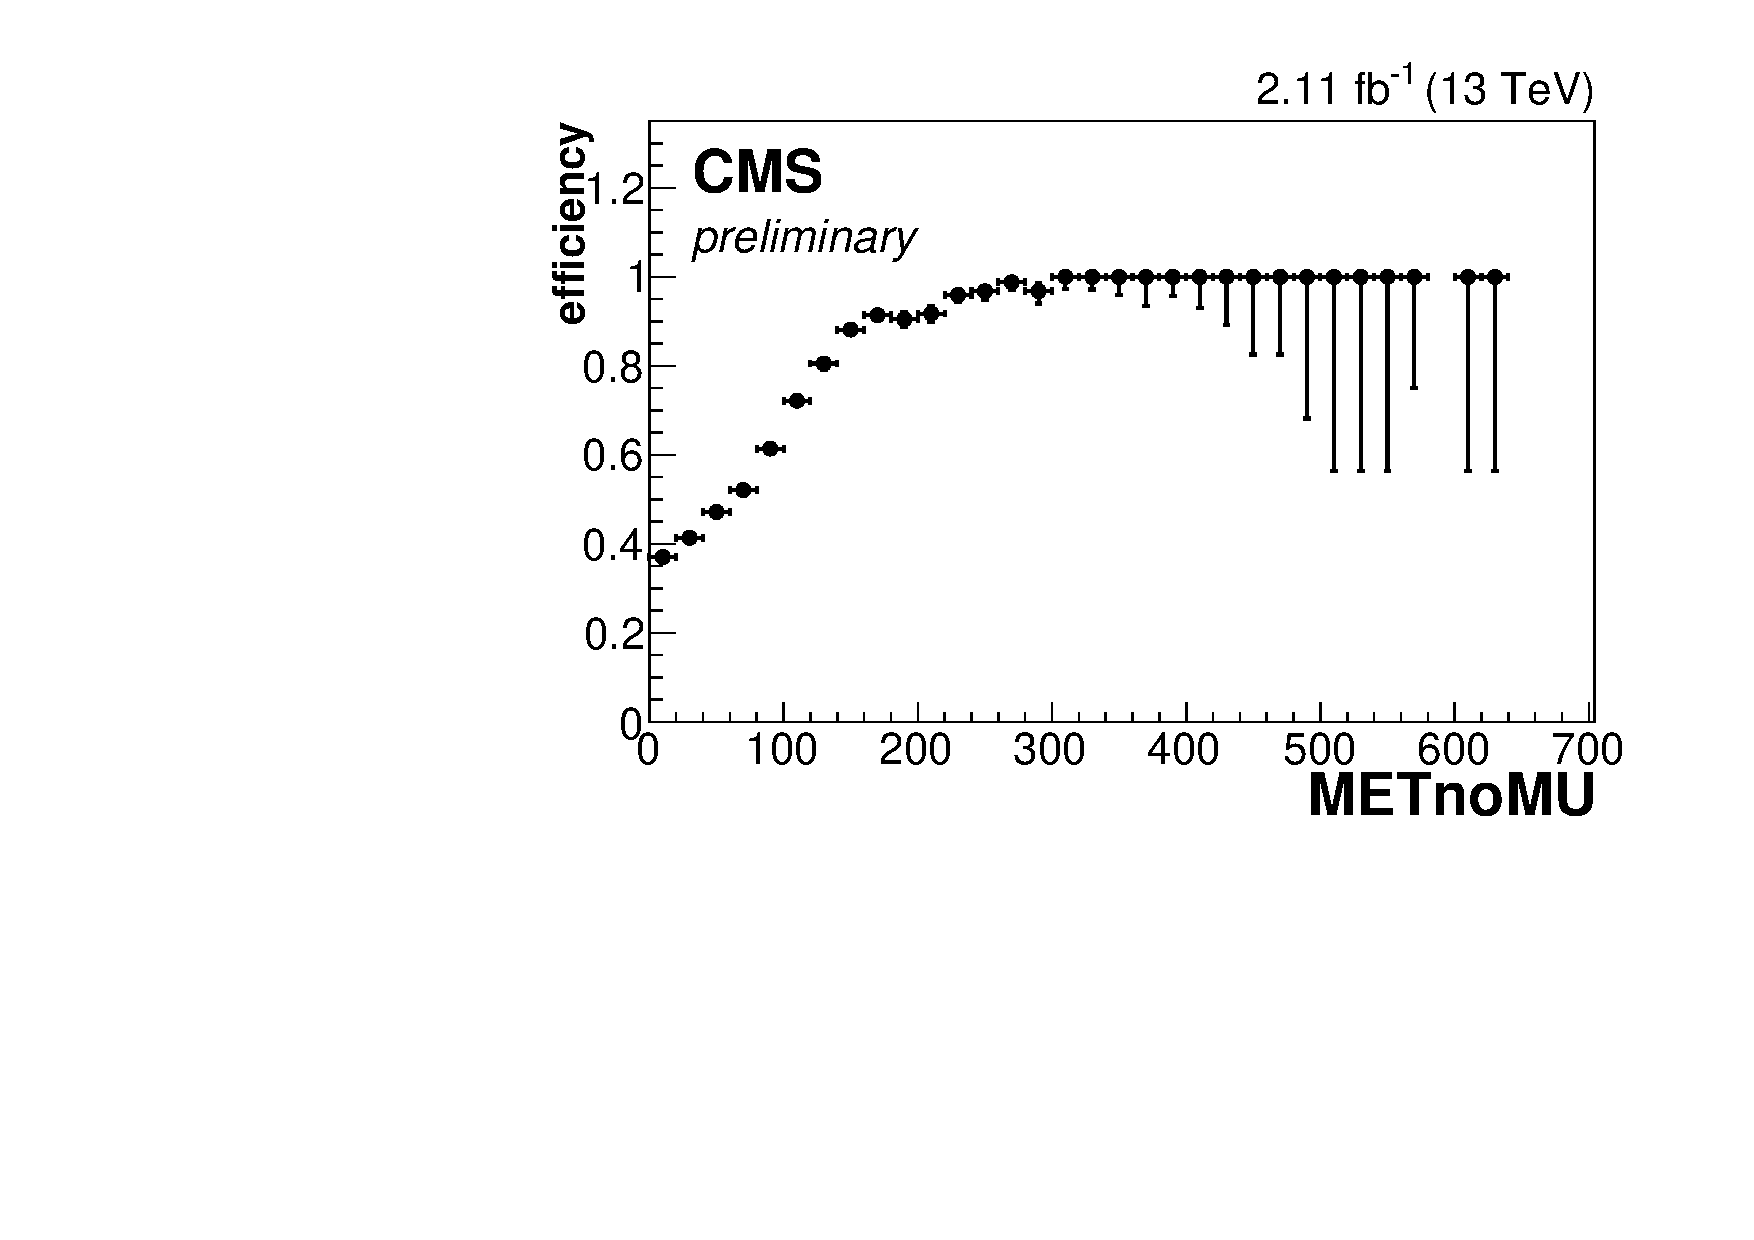
\includegraphics[width=.5\textwidth]{TalkPics/trigeff301115/output_2015Dtrigeff_131115json_l1etm60_vbfphasespace_301115/nunu_metnomuons.pdf}
\end{frame}

\begin{frame}
  \frametitle{L1ETM60 Efficiency: VBF phase space}
  \scriptsize
  \begin{block}{}
    \begin{itemize}
    \item L1 MET only sums up to $|\eta|=$3, shelf seen on previous slide could be due to jets in the HF
    \item Add requirement that both jets have $|\eta|<3$ to the denominator
    \item Good turn on recovered so shelf is due to events with jets in the HF
    \end{itemize}
  \end{block}
  \centering
  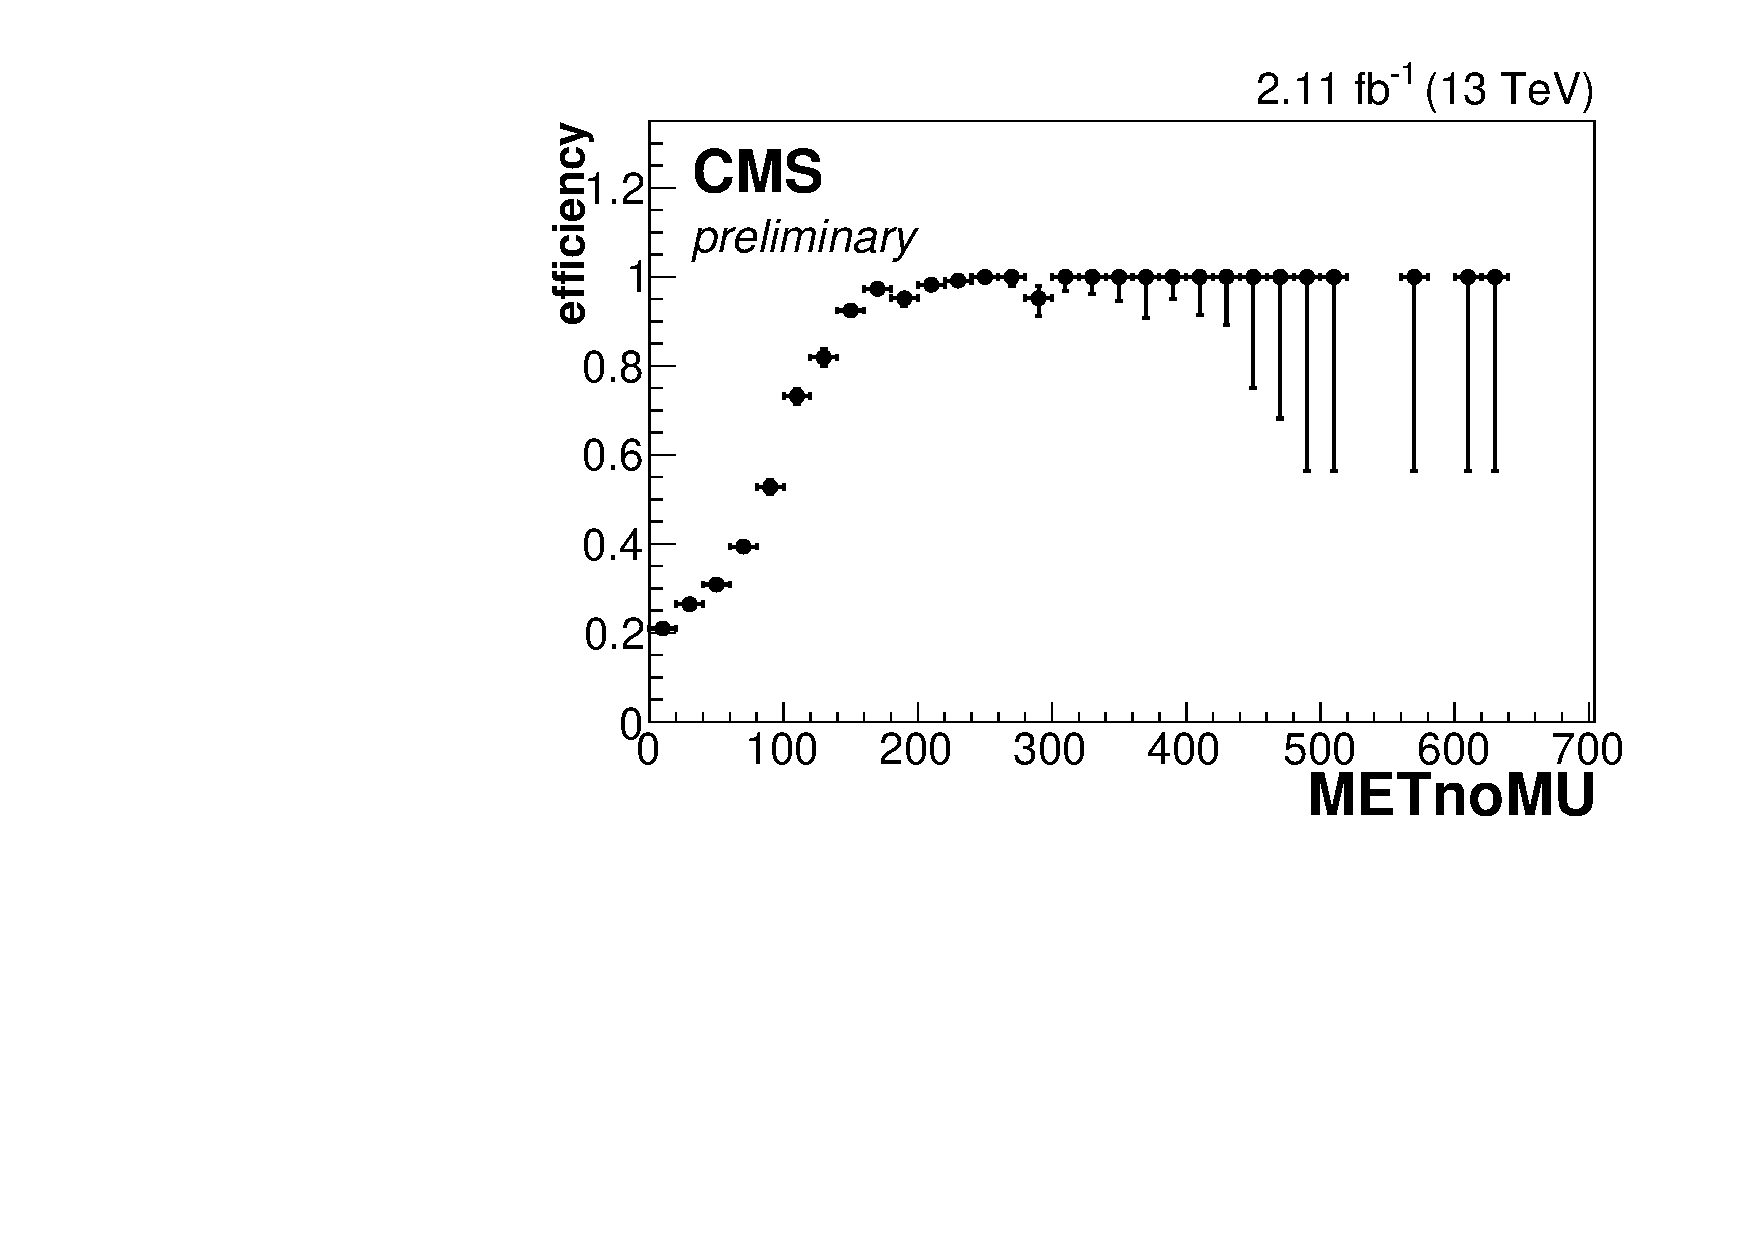
\includegraphics[width=.5\textwidth]{TalkPics/trigeff301115/output_2015Dtrigeff_131115json_l1etm60_vbfphasespace_bothcentral_301115/nunu_metnomuons.pdf}
\end{frame}



\begin{frame}
  \frametitle{Signal trigger turn on: MET}
  \scriptsize
  \vspace{-.3cm}
  \begin{block}{}
    \begin{itemize}
    \item Measure HLT efficiency (left) and L1+HLT efficiency (right)
    \item Dataset: Full 2015D data with latest JECv6
    \item Trigger: HLT\_DiPFJet40\_DEta3p5\_MJJ600\_PFMETNoMu140
    \item Denominator: SingleMuon events with dijet $p_{T}>80$, $M_{jj}>600$, $\Delta\eta_{jj}>3.6$ plus for left plot only L1ETM60
    \item[-] Jet pt cut very high due to slow jet pt turn on
    \item HLT only efficiency slightly better
    \end{itemize}
  \end{block}
  \centering
%  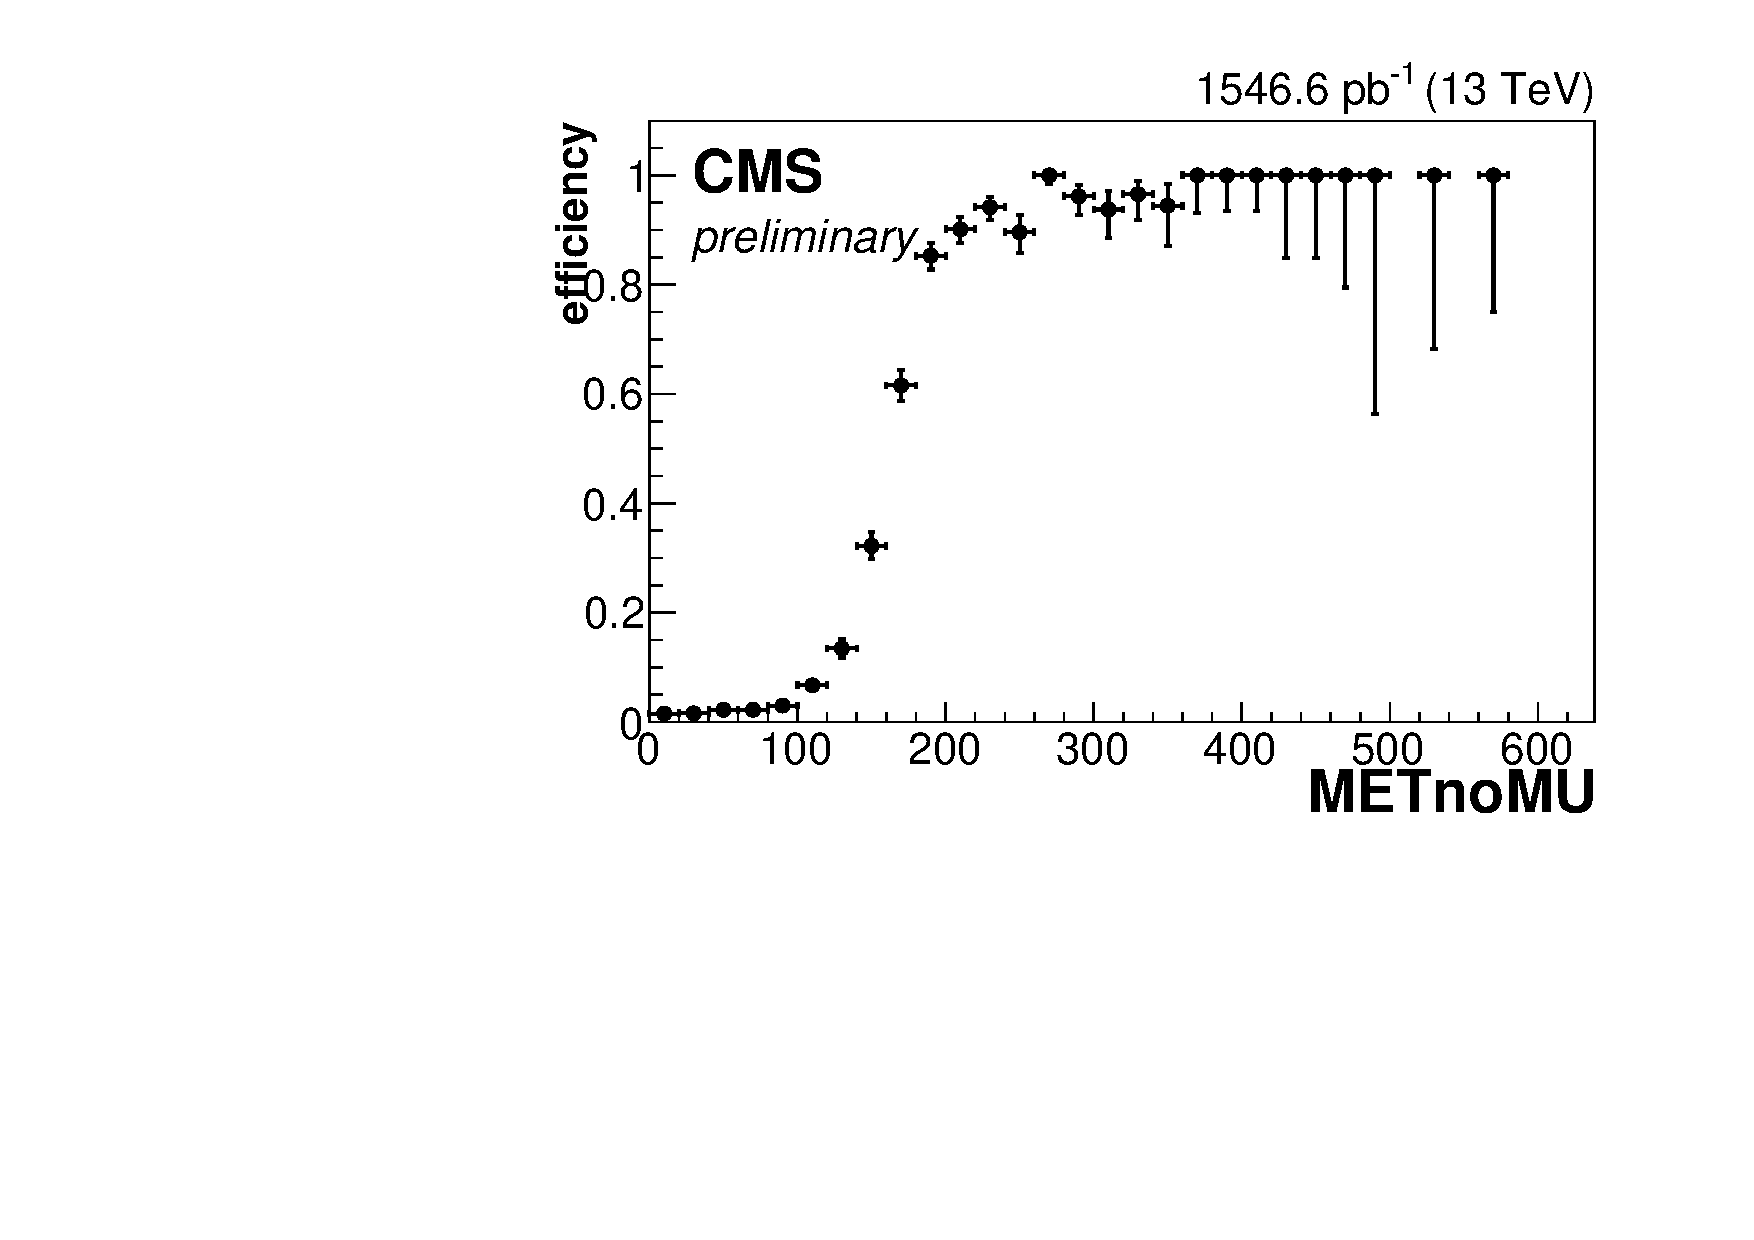
\includegraphics[width=.5\textwidth]{TalkPics/trigeff161115/output_2015Dtrigeff_301015json_sigtrig_l1met60met300jpt80cut_161115/nunu_metnomuons.pdf}
%  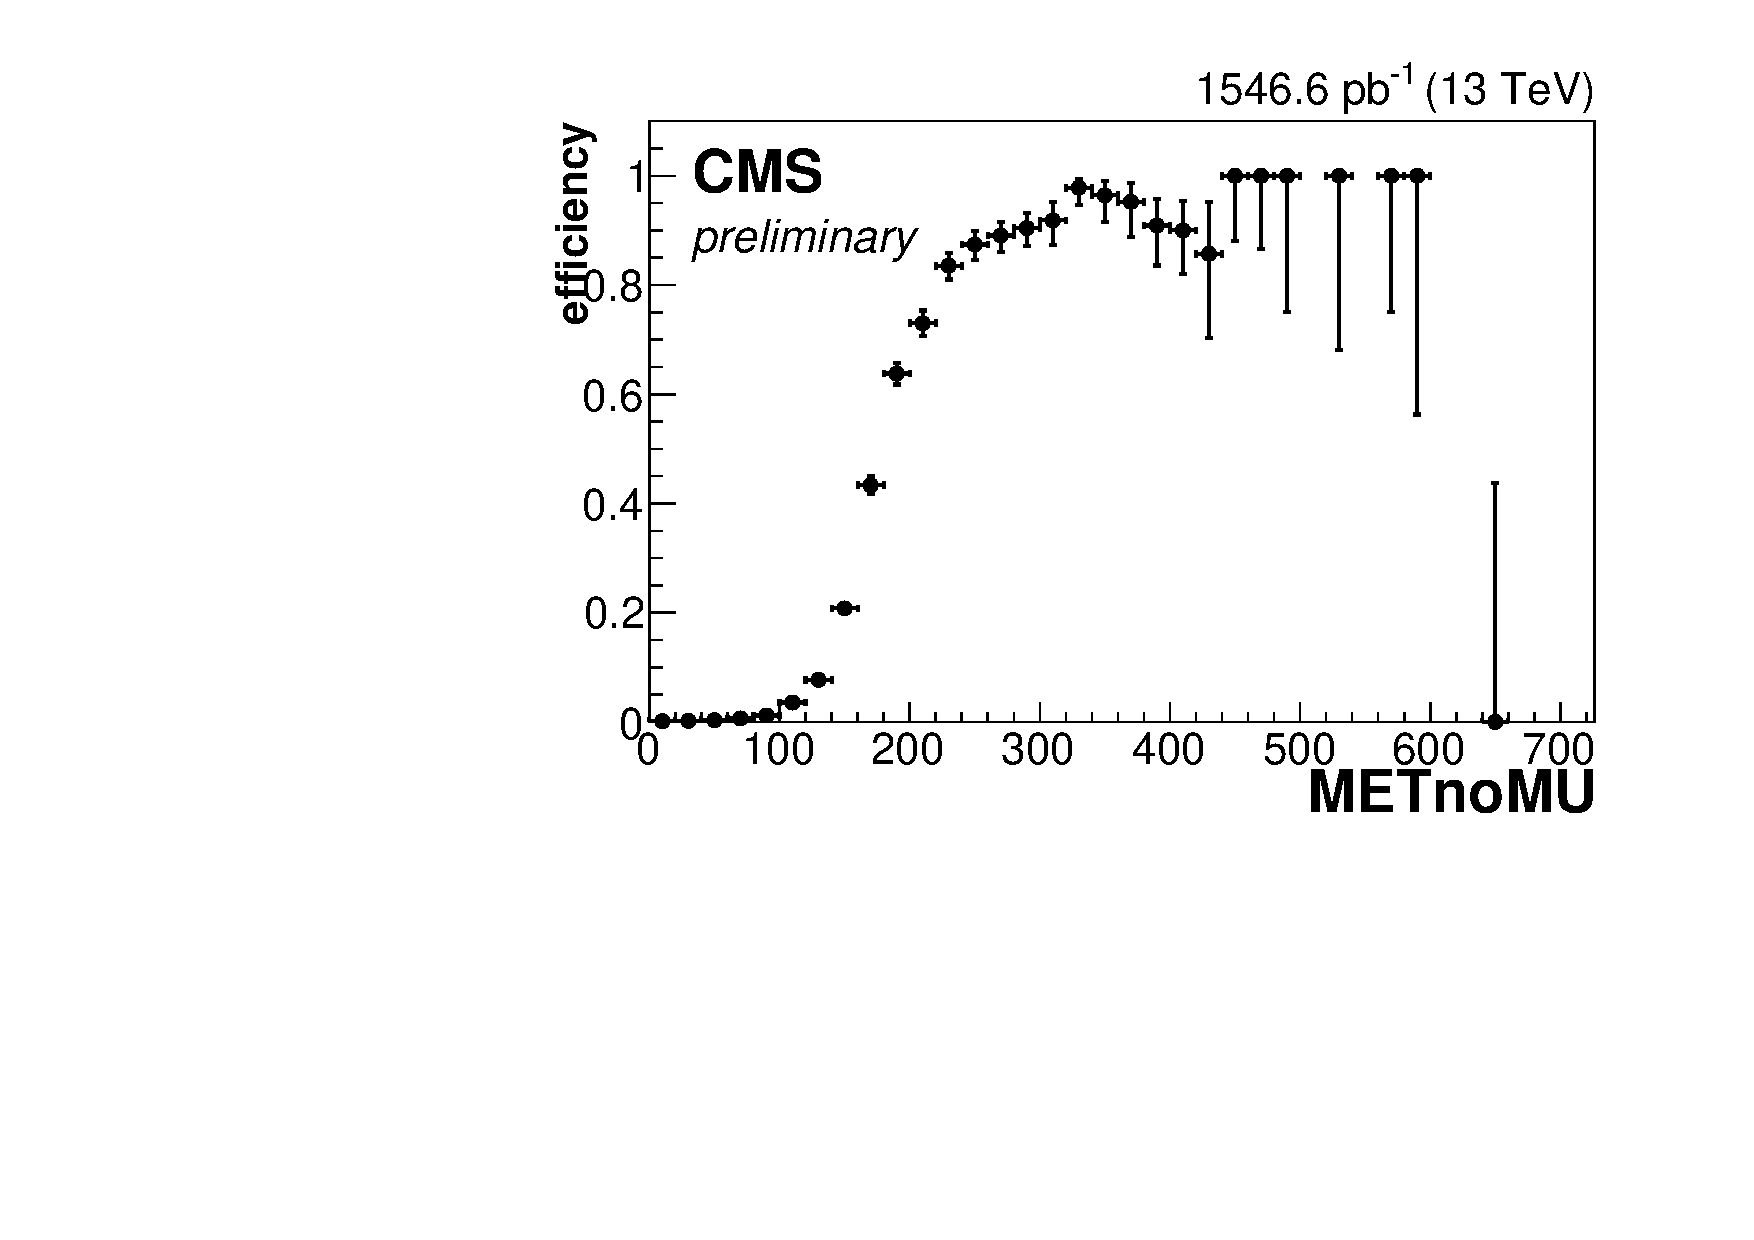
\includegraphics[width=.5\textwidth]{TalkPics/trigeffandpheno041115/nunu_metnomuons.pdf}
  \centering
   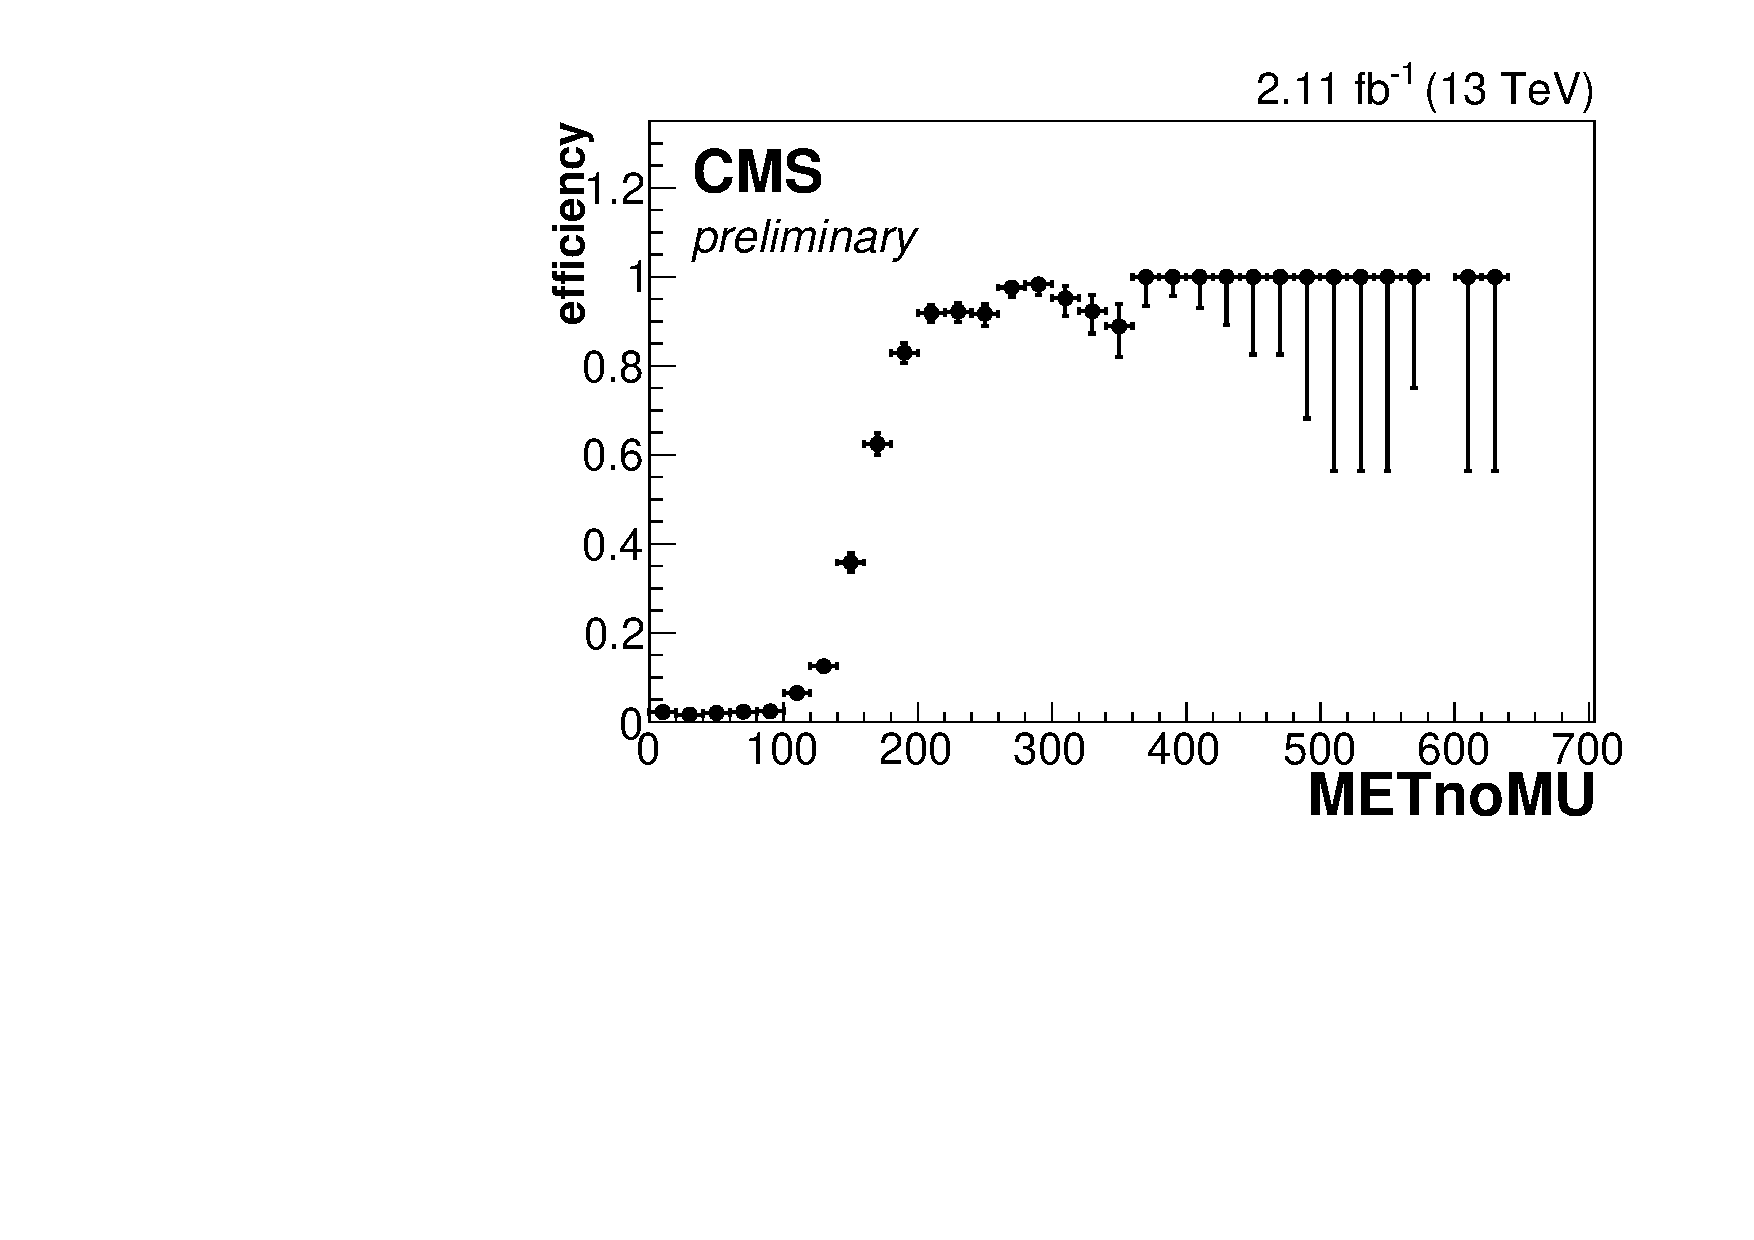
\includegraphics[width=.45\textwidth]{TalkPics/trigeff301115/output_2015Dtrigeff_131115json_sigtrig_hltonly_301115/nunu_metnomuons.pdf}
   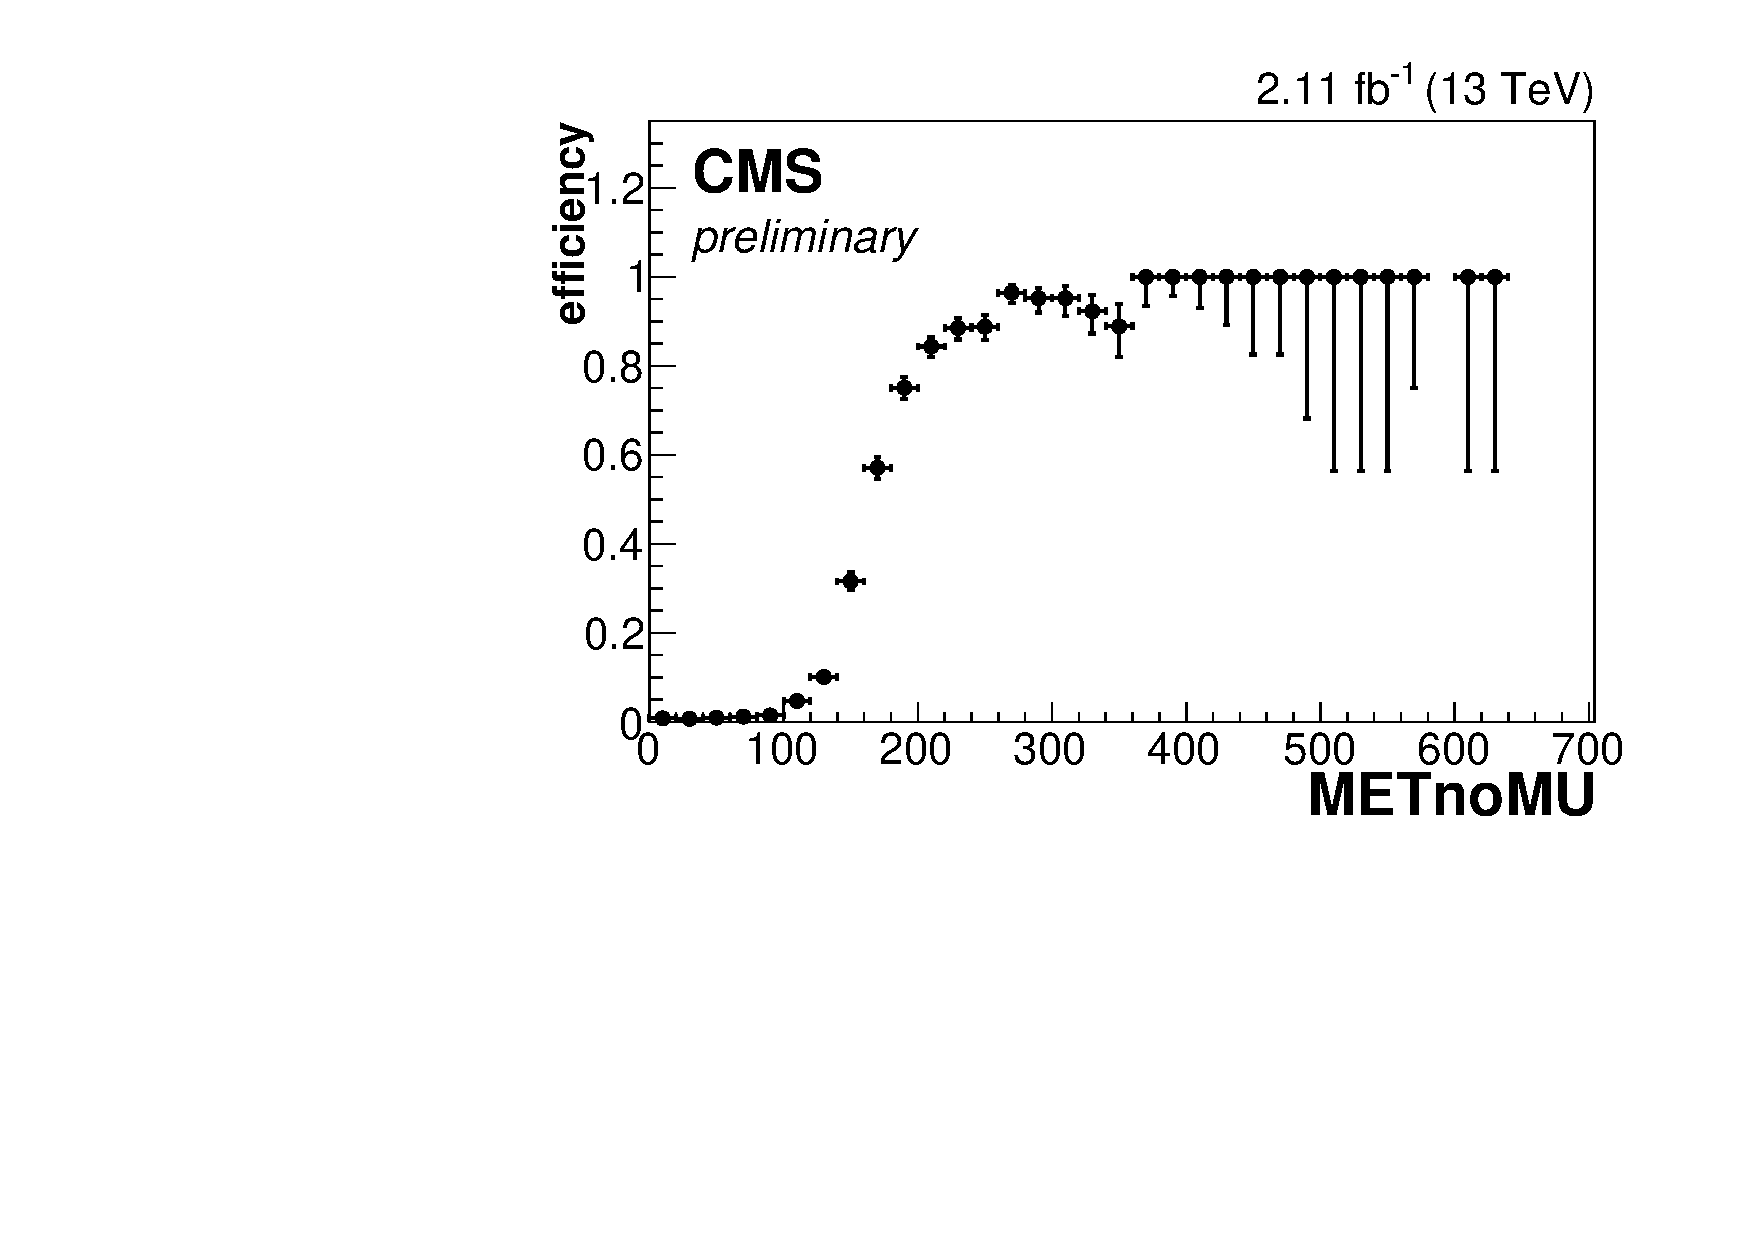
\includegraphics[width=.45\textwidth]{TalkPics/trigeff301115/output_2015Dtrigeff_131115json_sigtrig_301115/nunu_metnomuons.pdf}
\end{frame}

\begin{frame}
  \frametitle{Signal trigger turn on: jet pt}
  \scriptsize
  \vspace{-.3cm}
  \begin{block}{}
    \begin{itemize}
    \item Measure HLT efficiency (left) and L1+HLT efficiency (right)
    \item Dataset: Full 2015D data with latest JECv6
    \item Trigger: HLT\_DiPFJet40\_DEta3p5\_MJJ600\_PFMETNoMu140
    \item Denominator: SingleMuon events with dijet pt$>80$, $METnoMU>300$, $M_{jj}>600$, $\Delta\eta_{jj}>3.6$ plus for left plot only and L1ETM60
    \item[-] MET cut very high due to slow MET turn on
    \item HLT only efficiency slightly better
    \end{itemize}
  \end{block}
  \centering
%  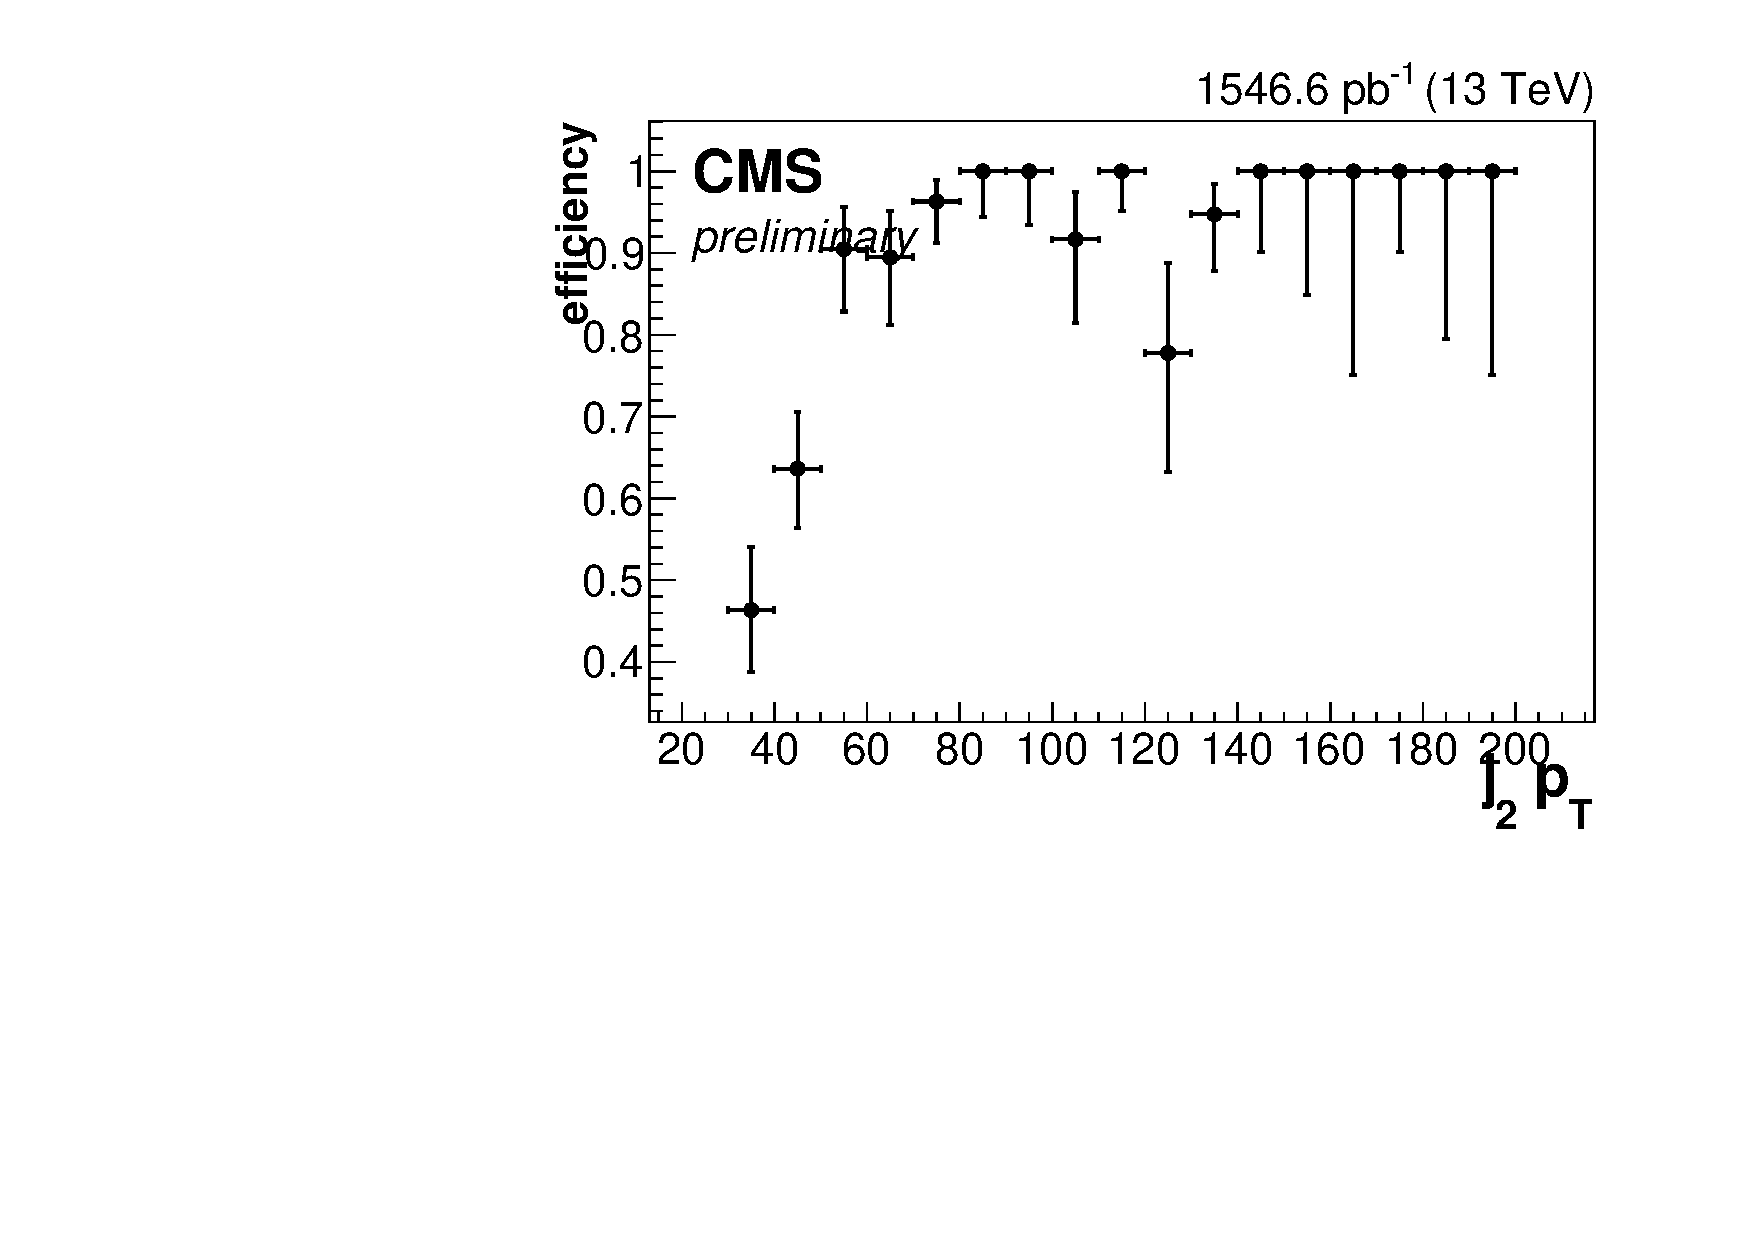
\includegraphics[width=.5\textwidth]{TalkPics/trigeff161115/output_2015Dtrigeff_301015json_sigtrig_l1met60met300jpt80cut_161115/nunu_jet2_pt.pdf}
%  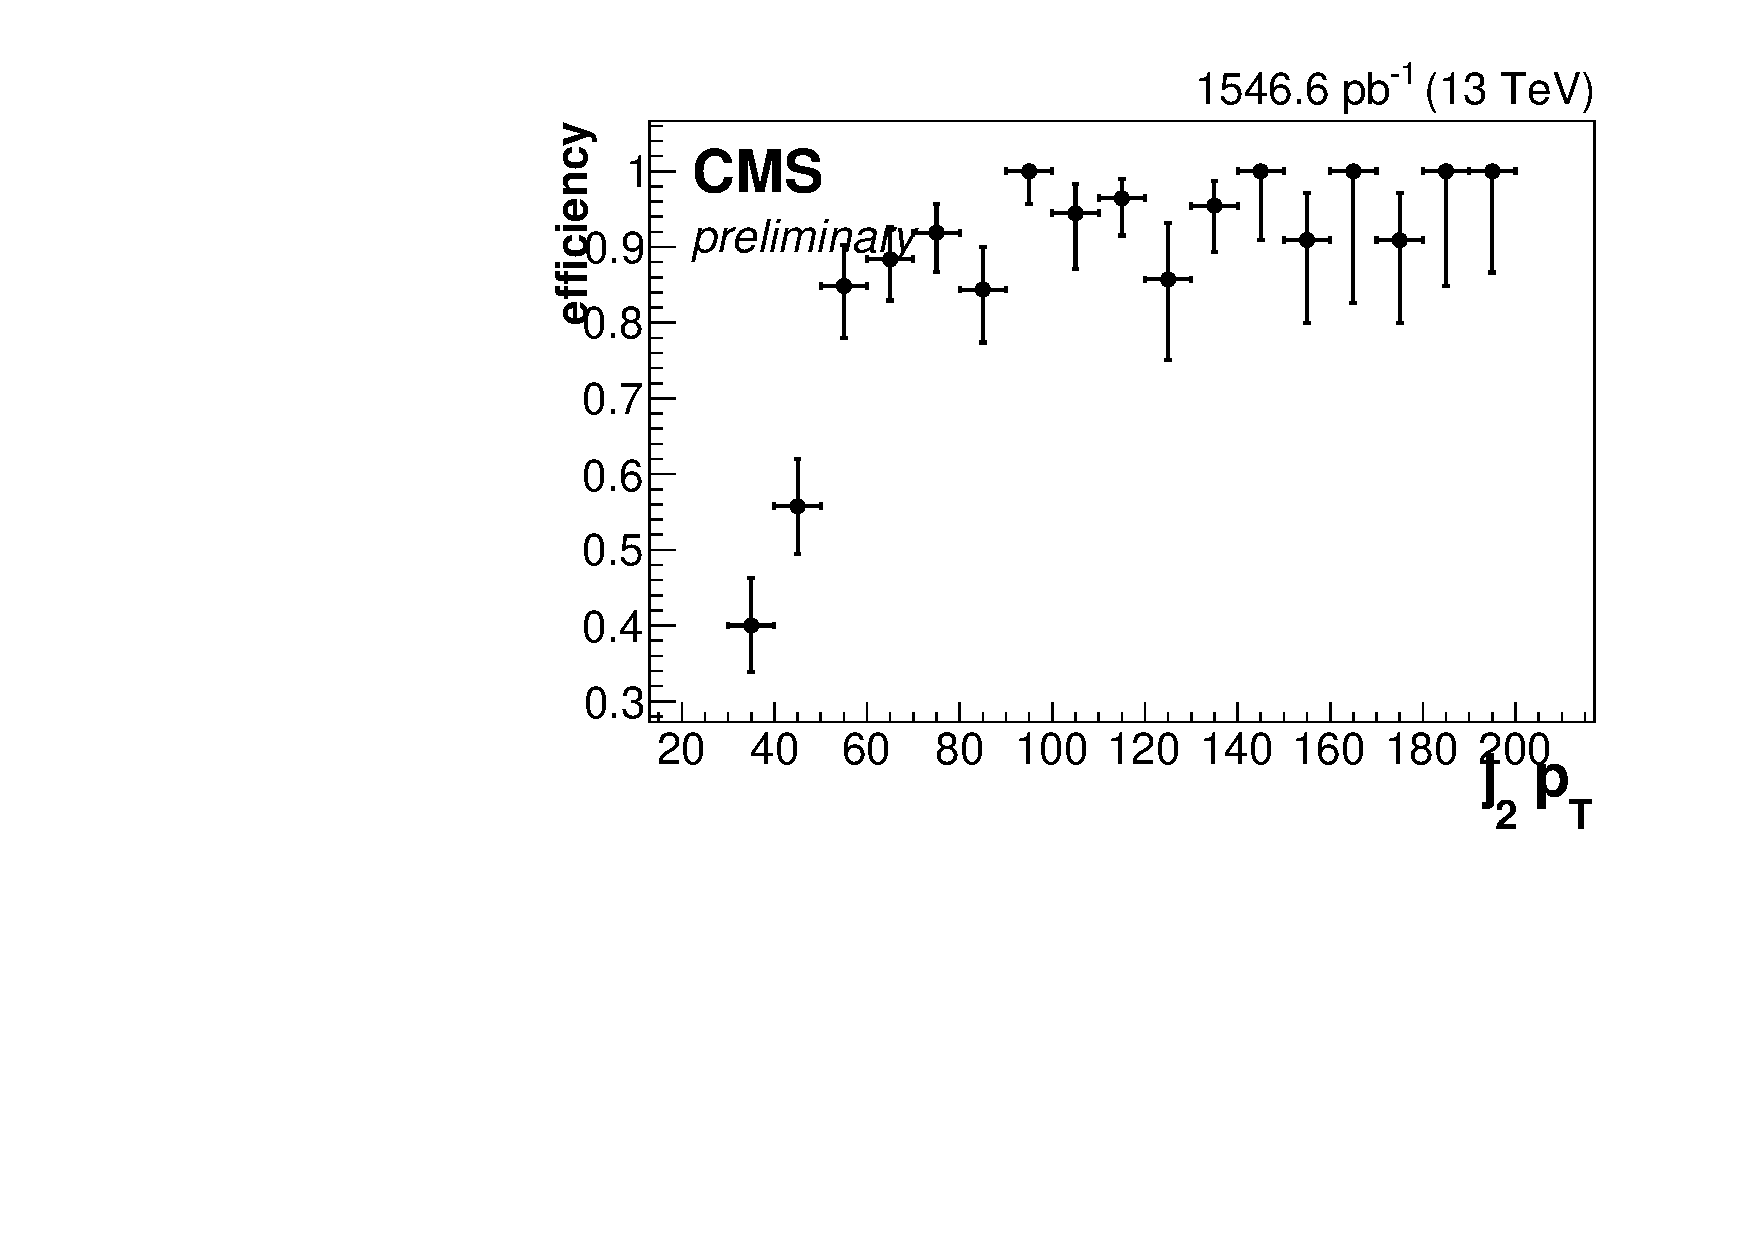
\includegraphics[width=.5\textwidth]{TalkPics/trigeffandpheno041115/nunu_jet2_pt.pdf}
  \centering
  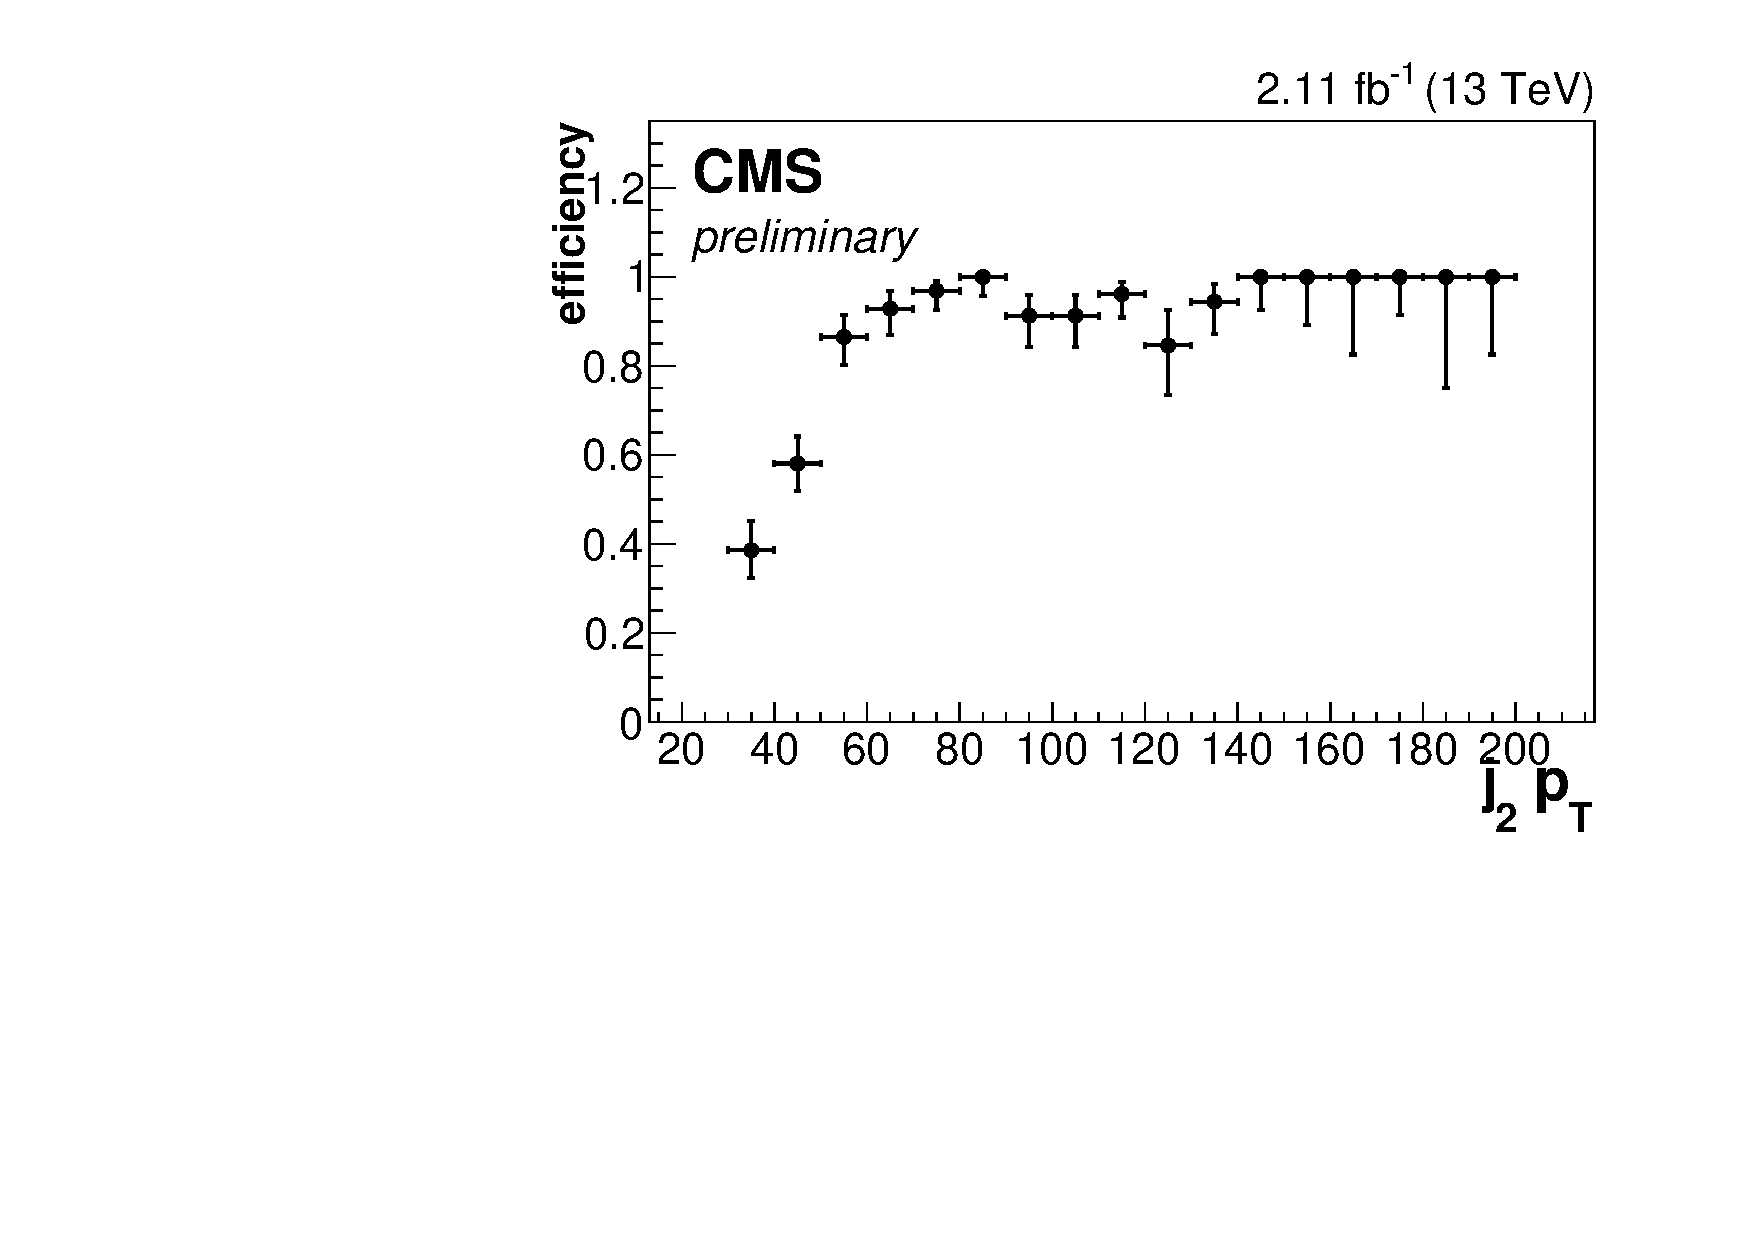
\includegraphics[width=.45\textwidth]{TalkPics/trigeff301115/output_2015Dtrigeff_131115json_sigtrig_hltonly_301115/nunu_jet2_pt.pdf}
  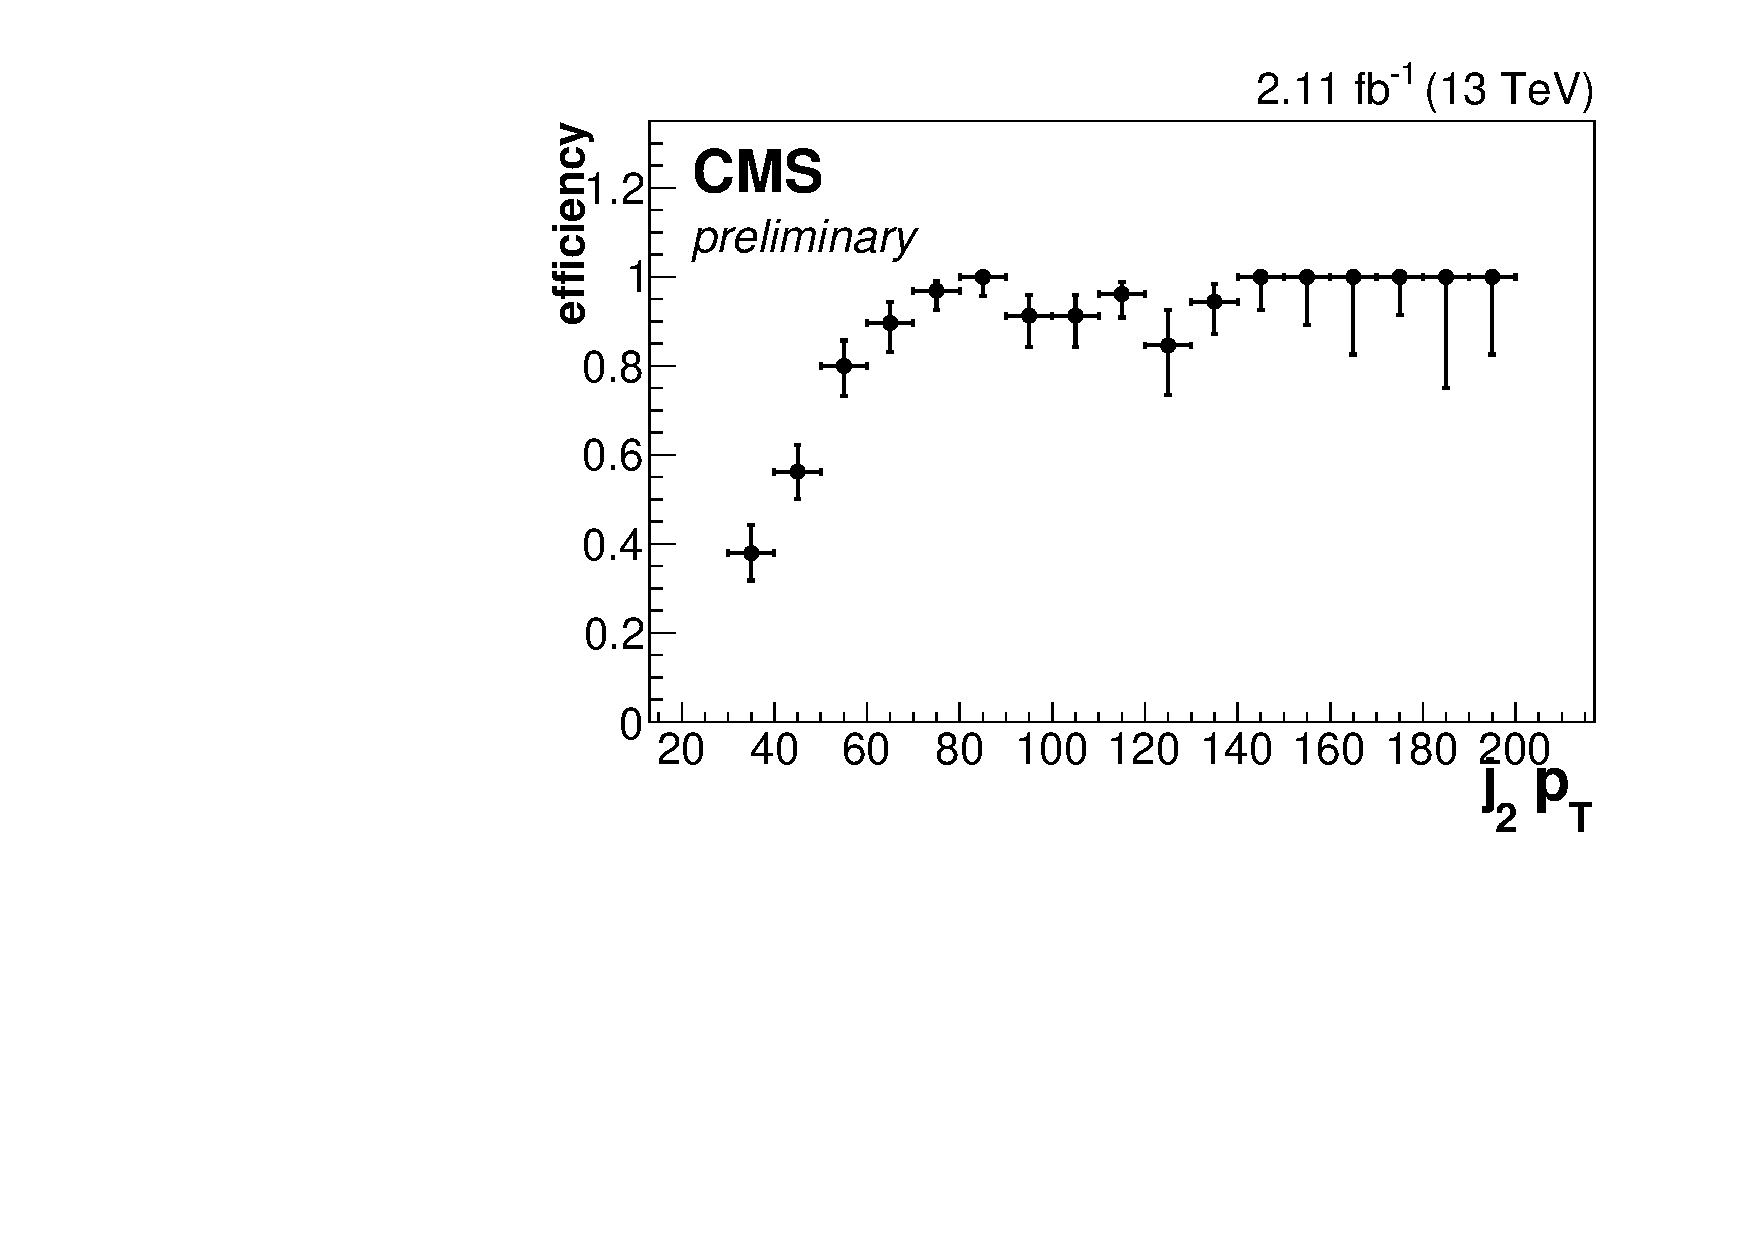
\includegraphics[width=.45\textwidth]{TalkPics/trigeff301115/output_2015Dtrigeff_131115json_sigtrig_301115/nunu_jet2_pt.pdf}
\end{frame}

\begin{frame}  
  \frametitle{Impact of L1MET inefficiencies on signal}
  \scriptsize
  \begin{block}{}
    \begin{itemize}
    \item Signal $\Delta\eta_{jj}$ higher than background so may be more affected by L1 inefficiency
    \item Check efficiencies in MC of HLT (red), L1 (black) and L1+HLT (green)
    \item MC sample: VBF\_HToInvisible\_M125\_13TeV\_powheg\_pythia8
    \item Denominator: dijet p$_T > 50$ GeV, M$_{jj} > 800$ GeV, $\Delta\eta_{jj} > 3.6$, METnoMU$>200$ GeV\\
    \item We lose a lot of signal due to L1 inefficiency
    \end{itemize}
  \end{block}
  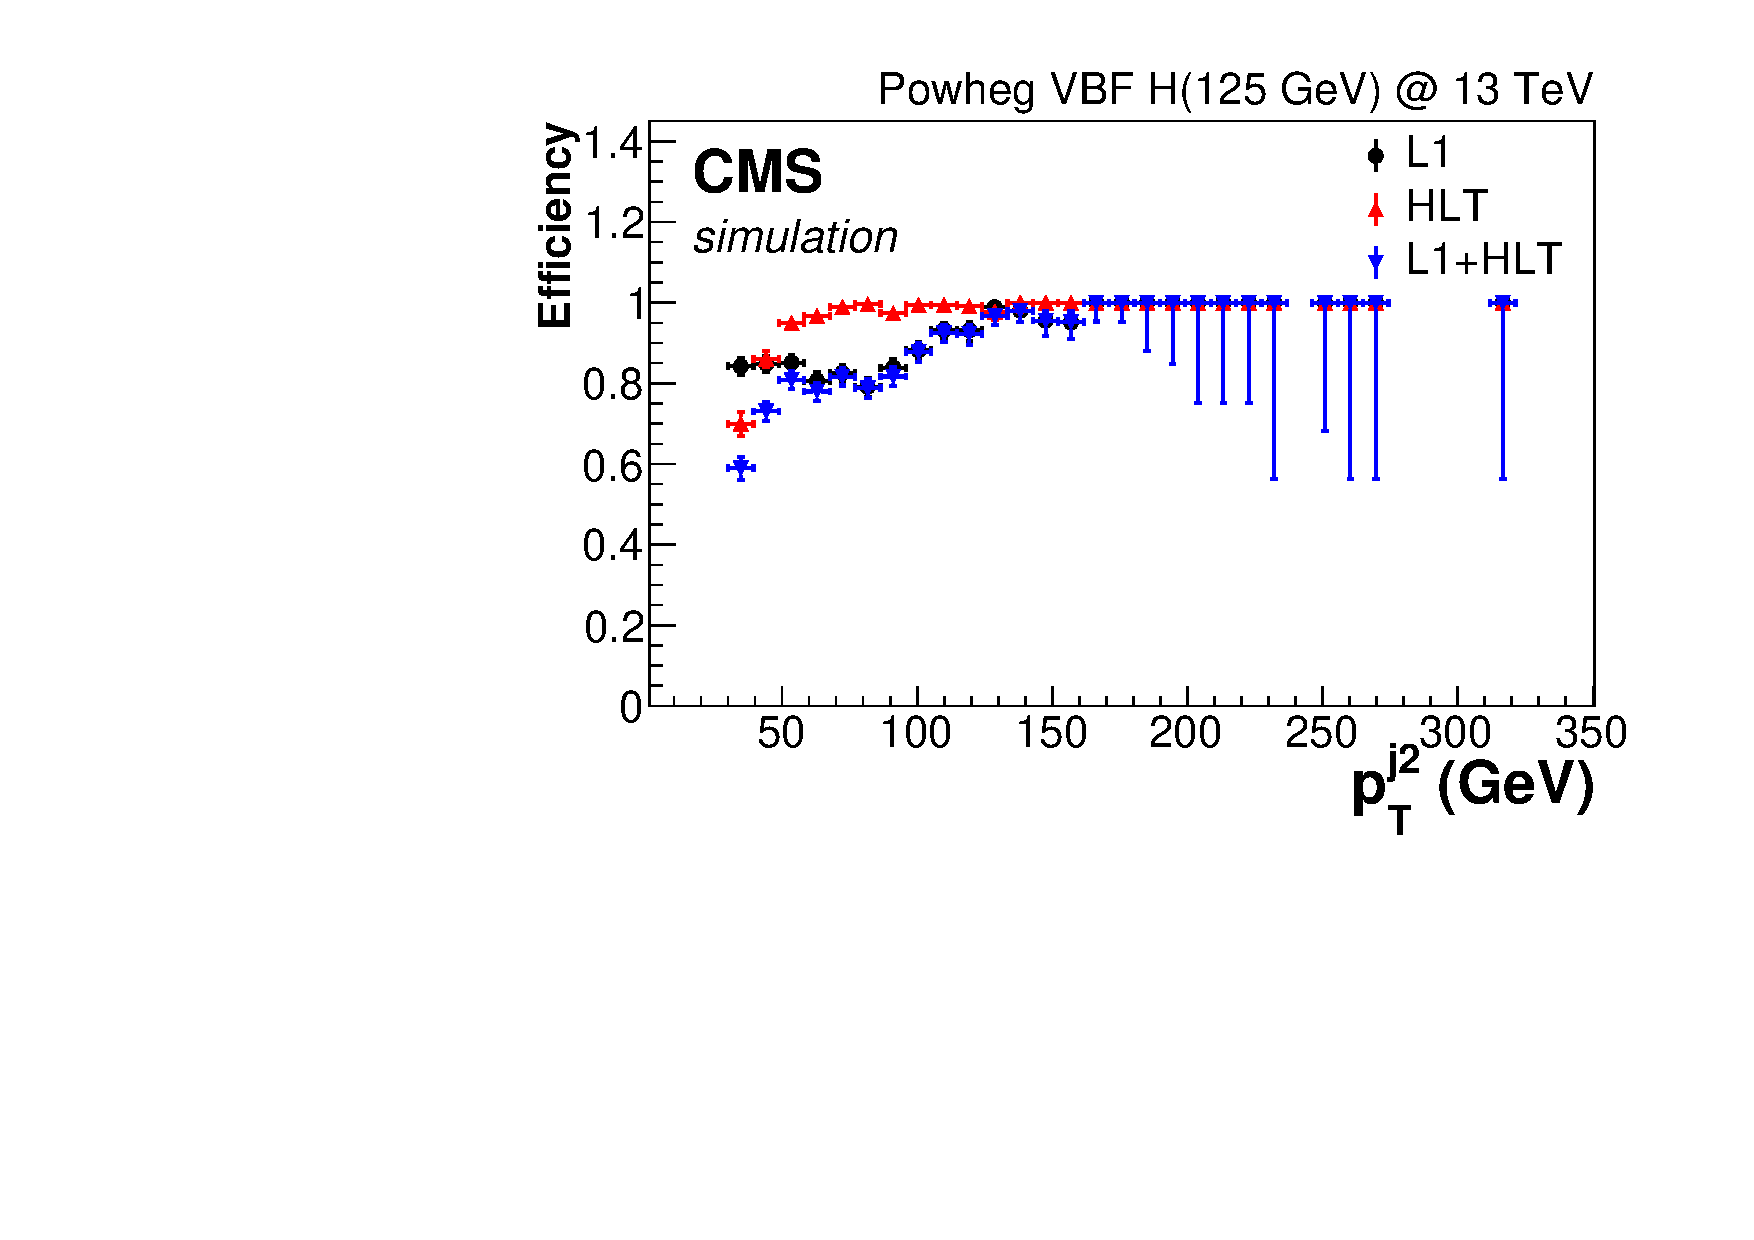
\includegraphics[width=.5\textwidth]{TalkPics/trigeff301115/SigTrigEff_jet2_pt.pdf}
  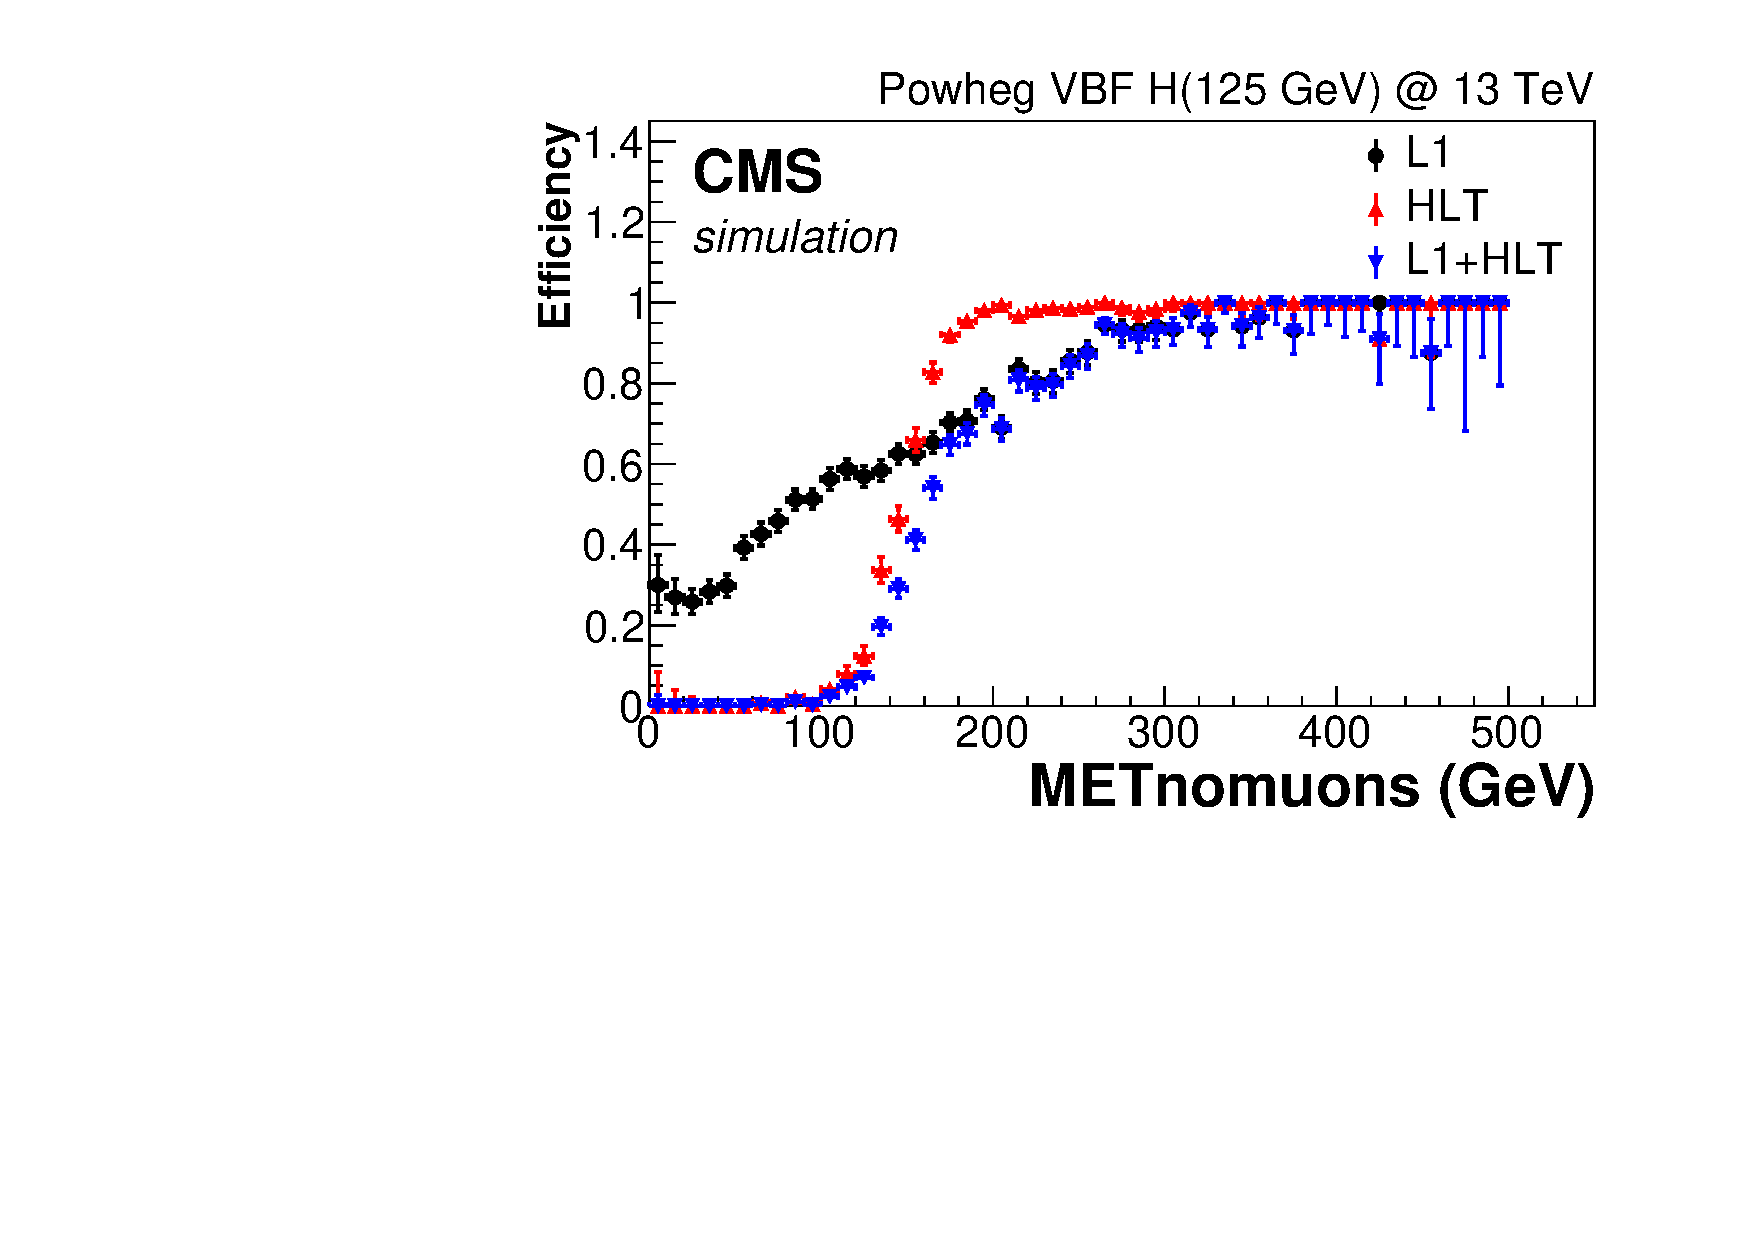
\includegraphics[width=.5\textwidth]{TalkPics/trigeff301115/SigTrigEff_metnomuons.pdf}
\end{frame}

\begin{frame}  
  \frametitle{Impact of L1MET inefficiencies on signal}
  \scriptsize
  \begin{block}{}
    \begin{itemize}
    \item Signal $\Delta\eta_{jj}$ higher than background so may be more affected by L1 inefficiency
    \item Check efficiencies in MC of HLT (red), L1 (black) and L1+HLT (green)
    \item MC sample: VBF\_HToInvisible\_M125\_13TeV\_powheg\_pythia8
    \item Denominator: dijet p$_T > 50$ GeV, M$_{jj} > 800$ GeV, $\Delta\eta_{jj} > 3.6$, METnoMU$>200$ GeV\\
    \item Inefficiency for jets in the HF can be clearly seen in the left plot
    \end{itemize}
  \end{block}
  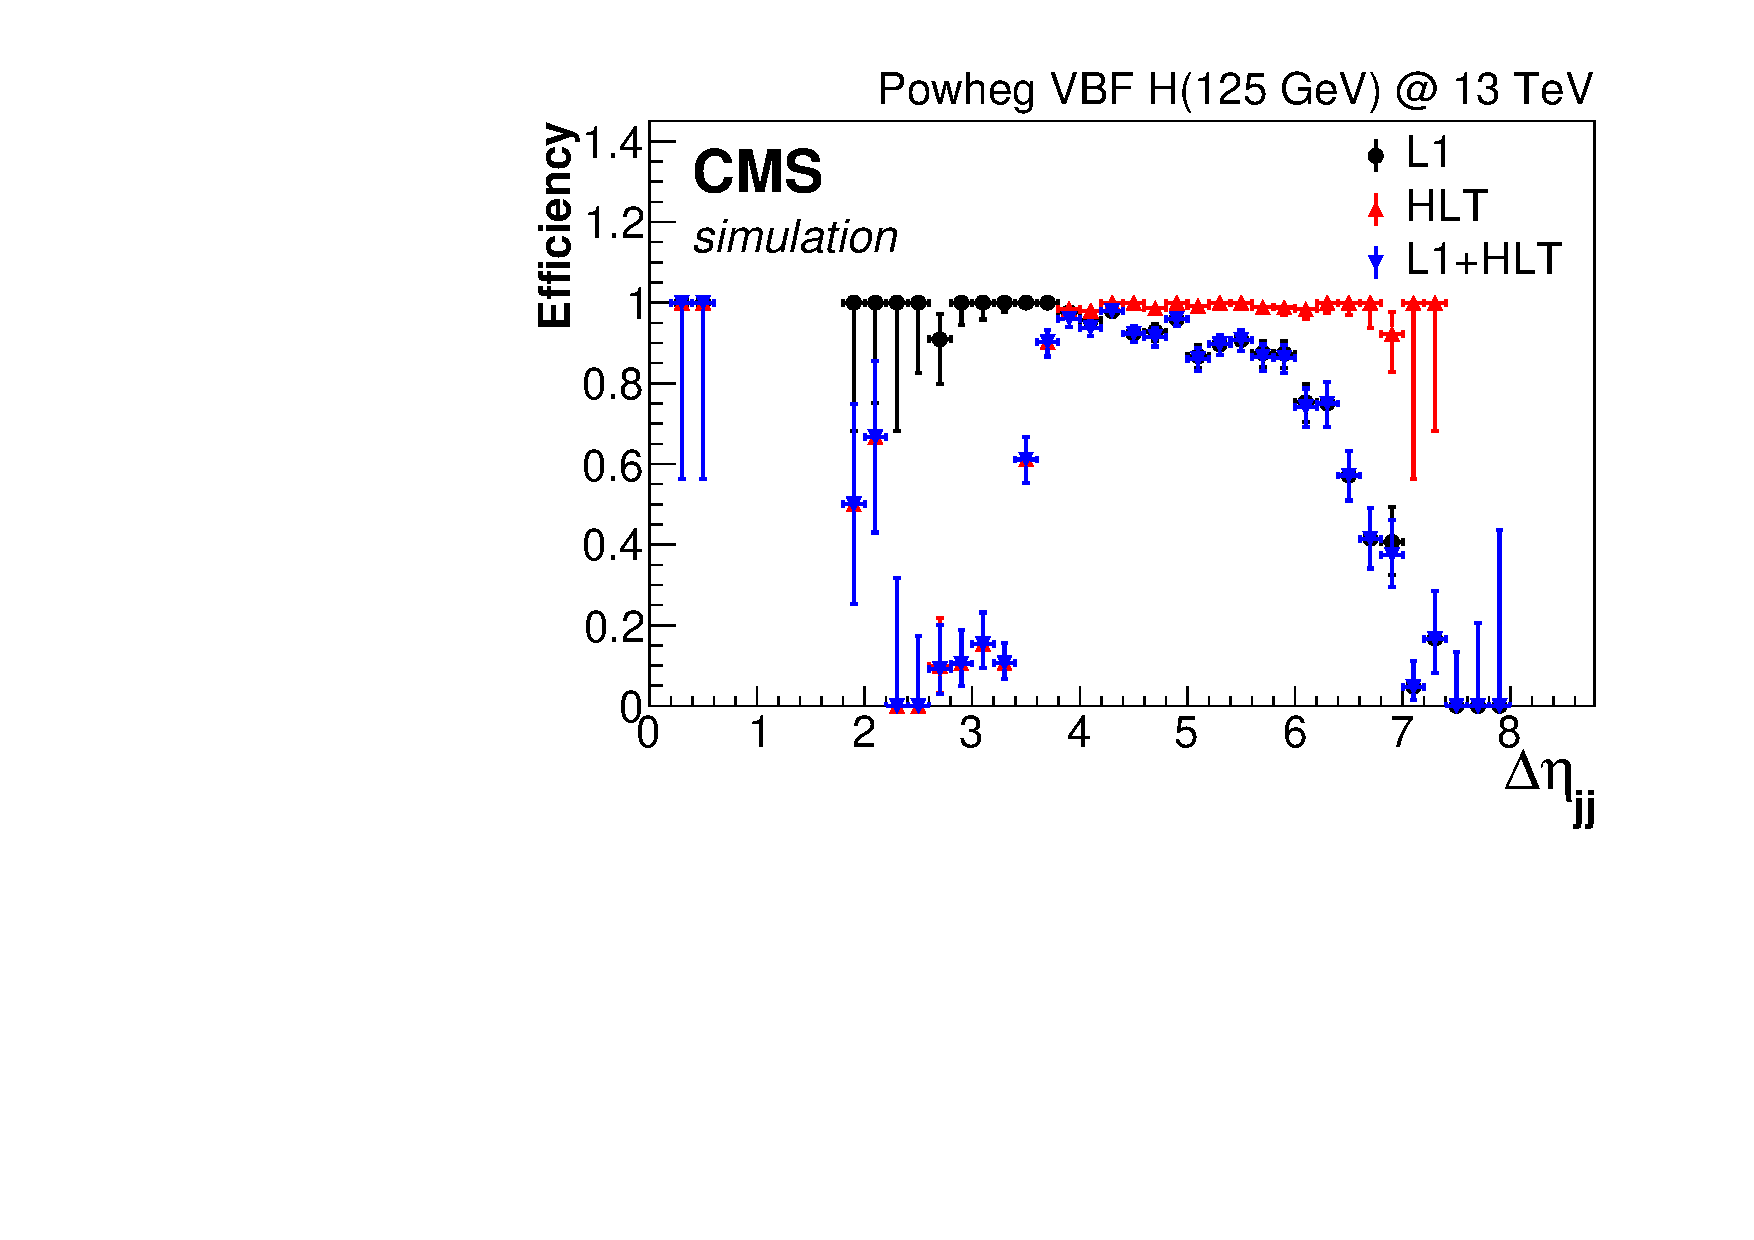
\includegraphics[width=.5\textwidth]{TalkPics/trigeff301115/SigTrigEff_dijet_deta.pdf}
  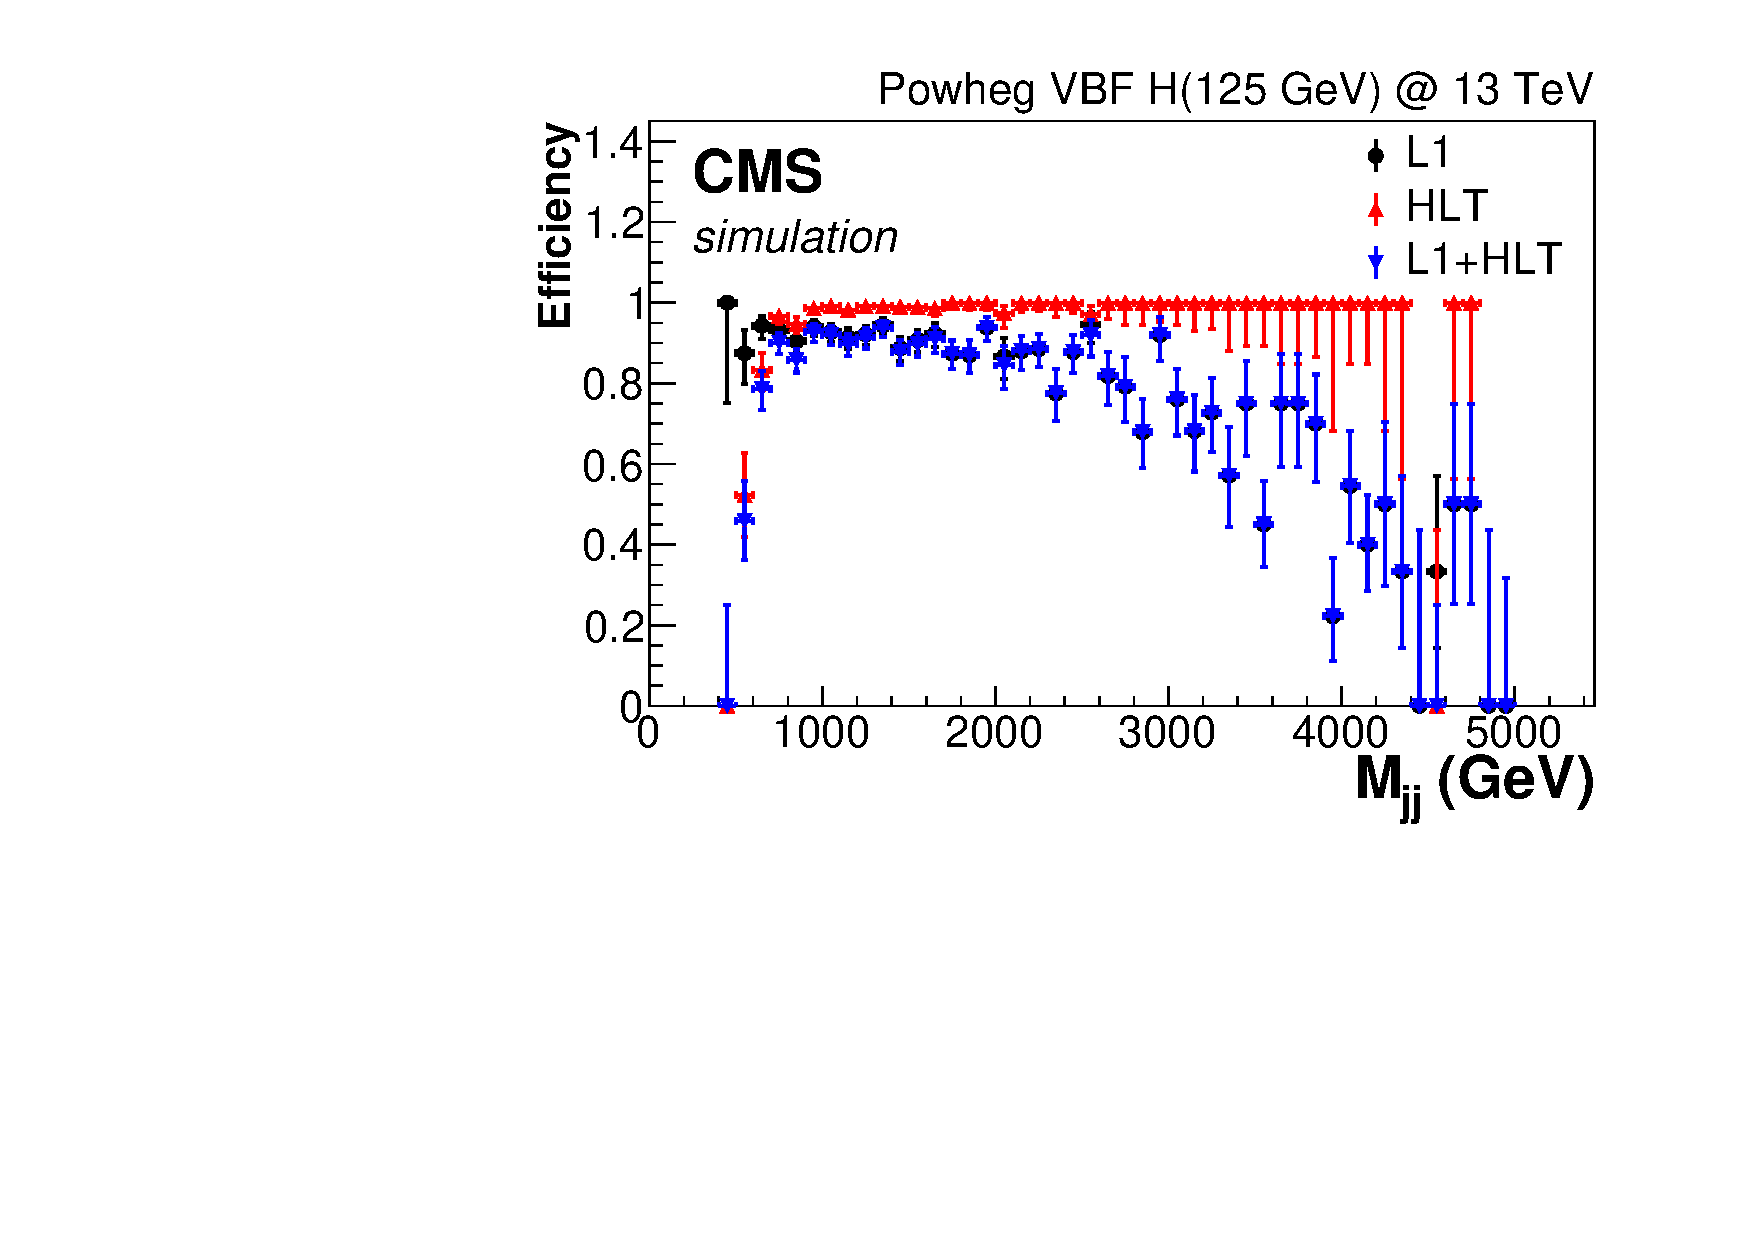
\includegraphics[width=.5\textwidth]{TalkPics/trigeff301115/SigTrigEff_dijet_M.pdf}
\end{frame}



\begin{frame}
  \frametitle{Calo jet prefilter}
  \scriptsize
  \begin{columns}
    \column{1.1\textwidth}
  \begin{block}{}
    \begin{itemize}
    \item Even after factoring out L1 effect jet pt is less efficient than in run 1
    \item According to \href{https://indico.cern.ch/event/456813/contribution/0/attachments/1178012/1704076/15-10-28_News_PPD.pdf}{these slides} wrong JEC was used in HLT during Run2015
    \item[-] We have a calo prefilter at 30 GeV
    \item[-] Calo JEC are large so wrong JEC could cause the remaining jet pt issues
    \item Plot offline jet pt (x axis) against trigger calo jet pt (y axis)
    \item Large differences seen between calo jet pt and offline pt
    \end{itemize}
  \end{block}
  \end{columns}
  \centering
  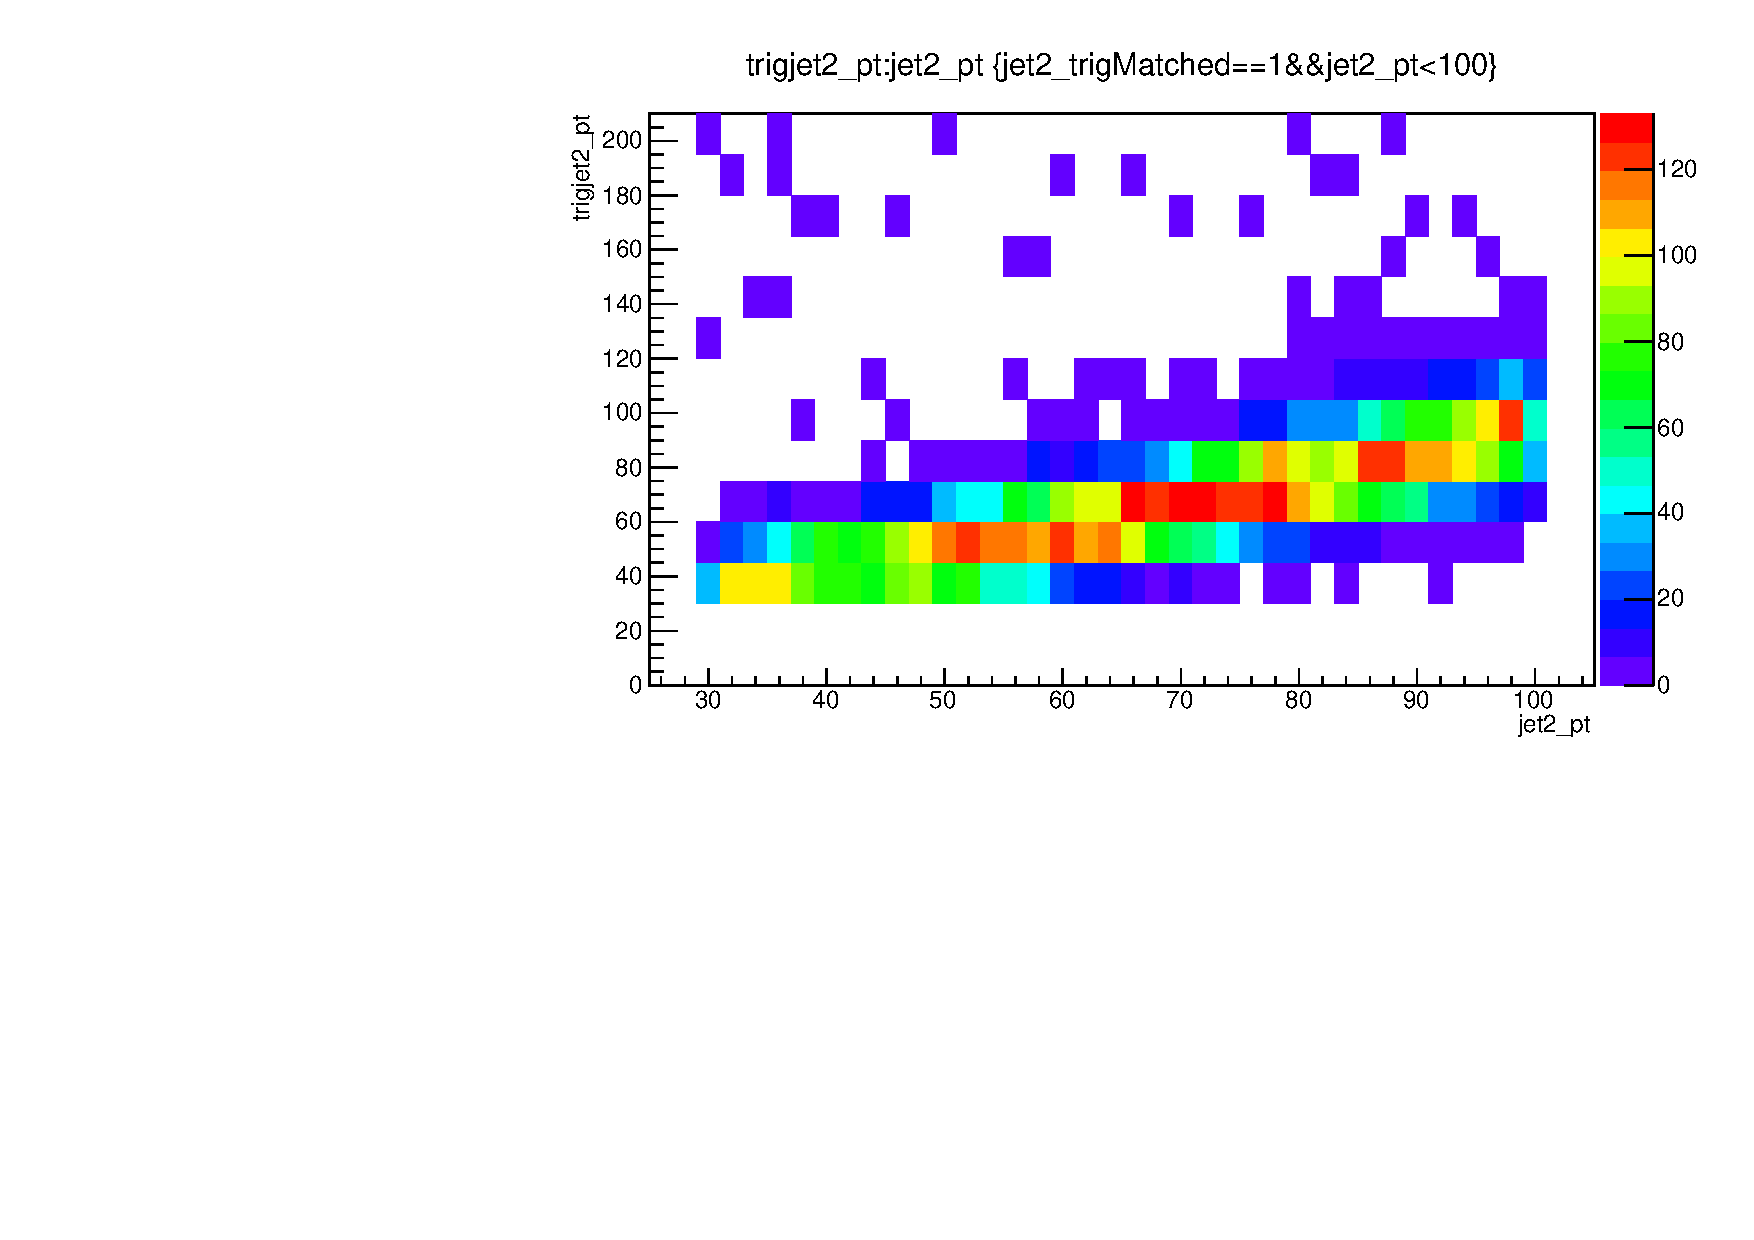
\includegraphics[width=.5\textwidth]{TalkPics/trigeff021115/trigeffstudies/jet2calotrigresponsept<100.pdf}
\end{frame}

\begin{frame}
  \frametitle{Calo jet prefilter}
  \scriptsize
  \begin{block}{}
    \begin{itemize}
    \item Further check, compare HLT efficiency in data (with wrong JEC) to that in MC (with correct JEC)
    \item MC sample: WJetsToLNu-mg and all the HT-binned samples
    \item Denominator: dijet p$_T > 50$ GeV, M$_{jj} > 800$ GeV, $Delta\eta_{jj} > 3.6$, METnoMU$>200$ GeV\\
    \item MC efficiency quite a bit better: more evidence wrong JEC could be to blame
    \end{itemize}
  \end{block}
  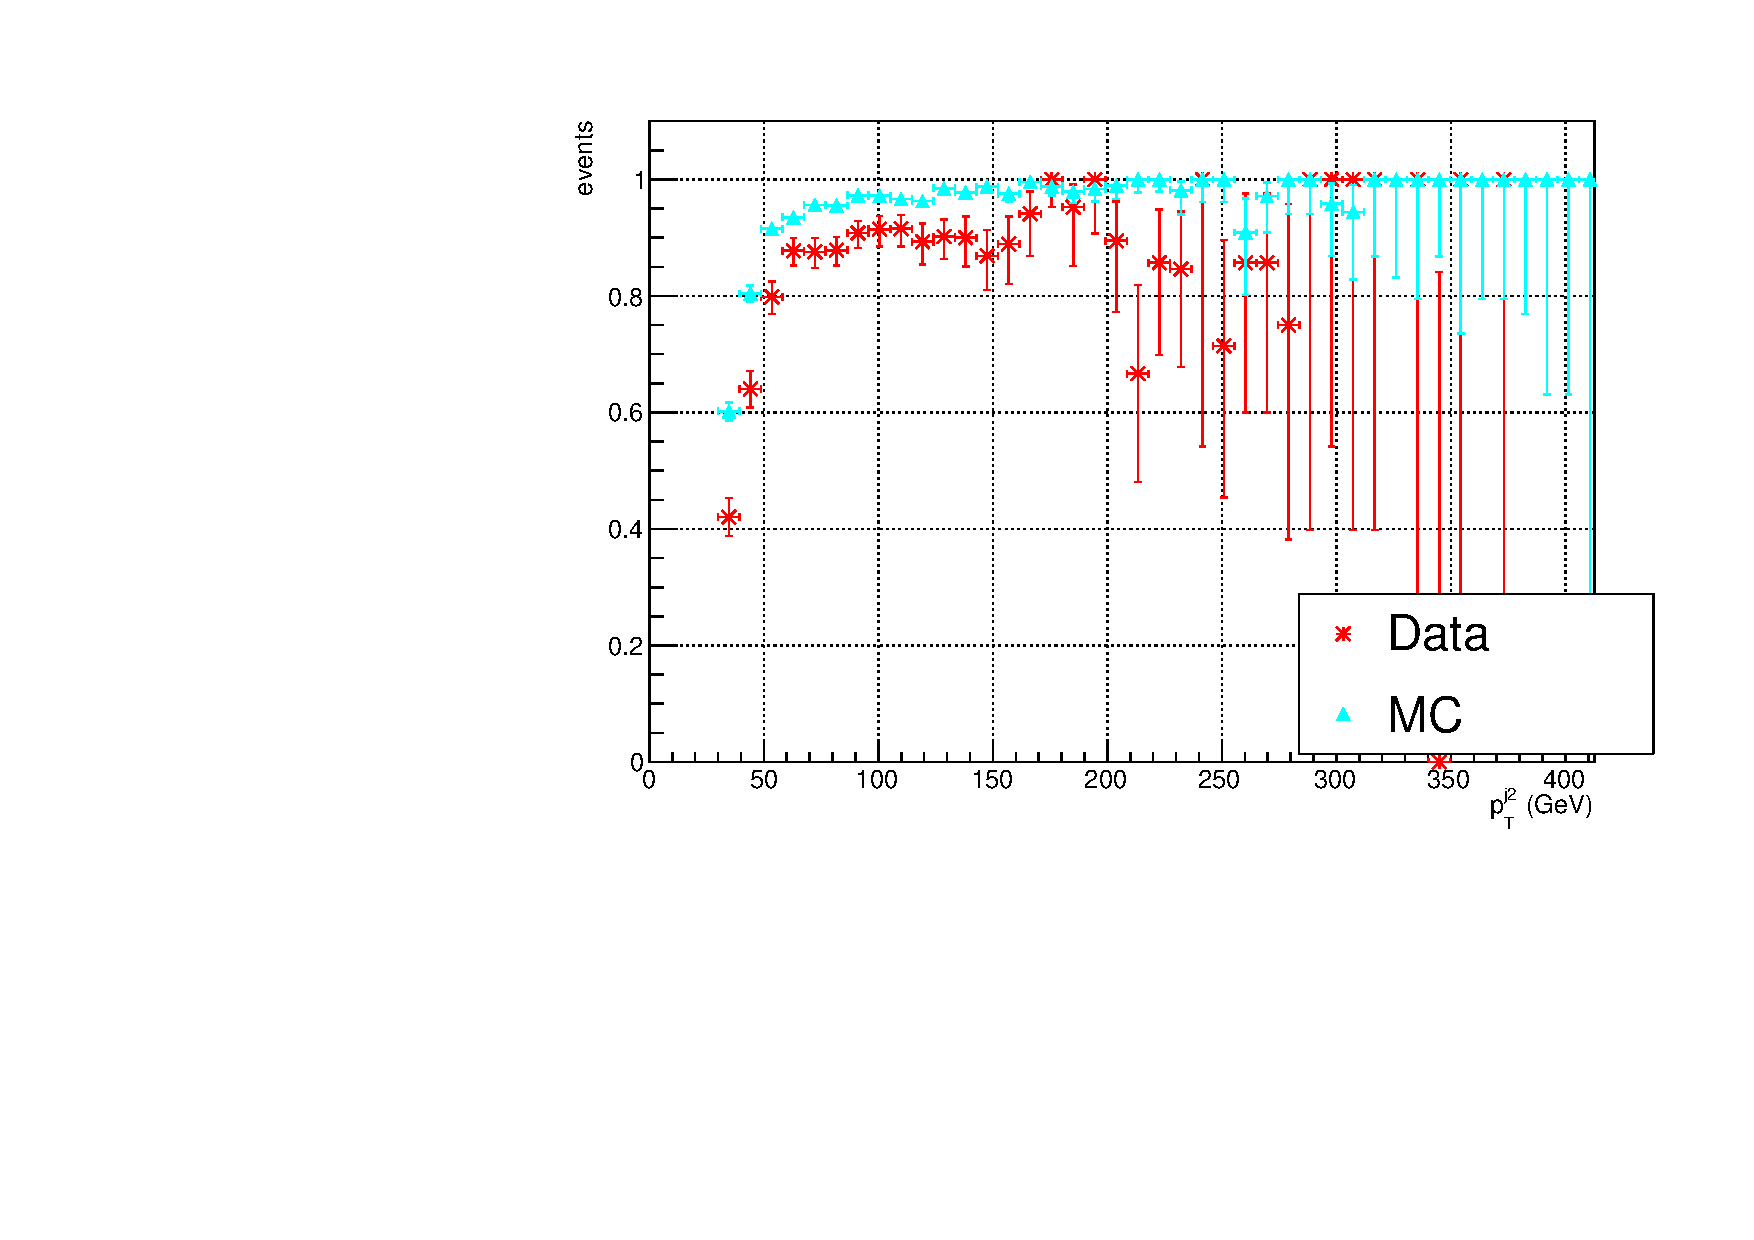
\includegraphics[width=.5\textwidth]{TalkPics/trigeff181115/DataMCHLTTrigEff_jet2_pt.pdf}
  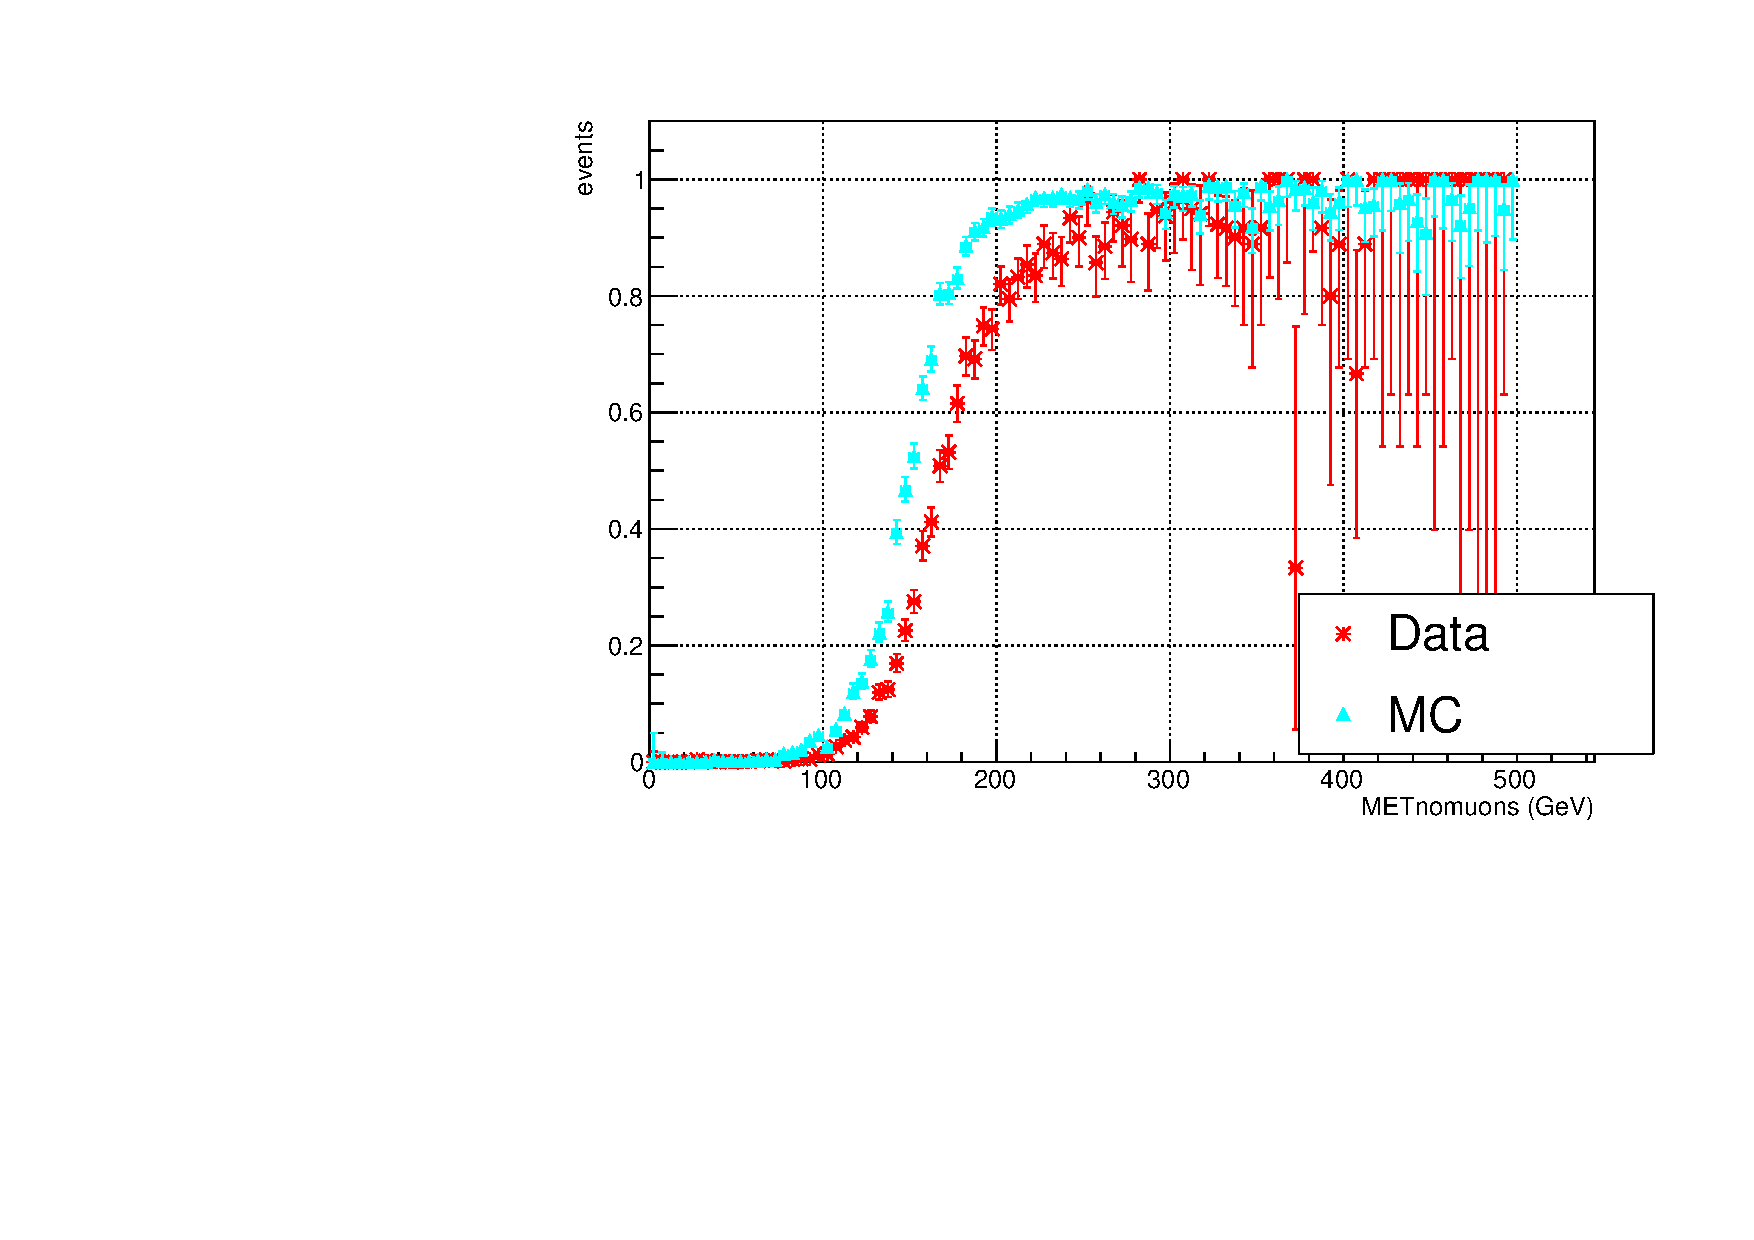
\includegraphics[width=.5\textwidth]{TalkPics/trigeff181115/DataMCHLTTrigEff_metnomuons.pdf}
\end{frame}

\begin{frame}
  \frametitle{Comparison with MET only trigger}
  \scriptsize
  \vspace{-.2cm}
  \begin{block}{}
    \begin{itemize}
    \item PF MET$>170$ GeV is the lowest unprescaled MET trigger
    \item Check efficiency in VBF region: dijet p$_T > 50$ GeV, M$_{jj} > 800$ GeV, $\Delta\eta_{jj} > 3.6$
    \item Efficiency for MET (left) looks good
    \item Efficiency for METnoMuons (right) is not so good:
    \item[-] Would significantly reduce control region statistics, currently the dominant error
    \item Our signal trigger is therefore important for maintaining analysis sensitivity

    \end{itemize}
  \end{block}
  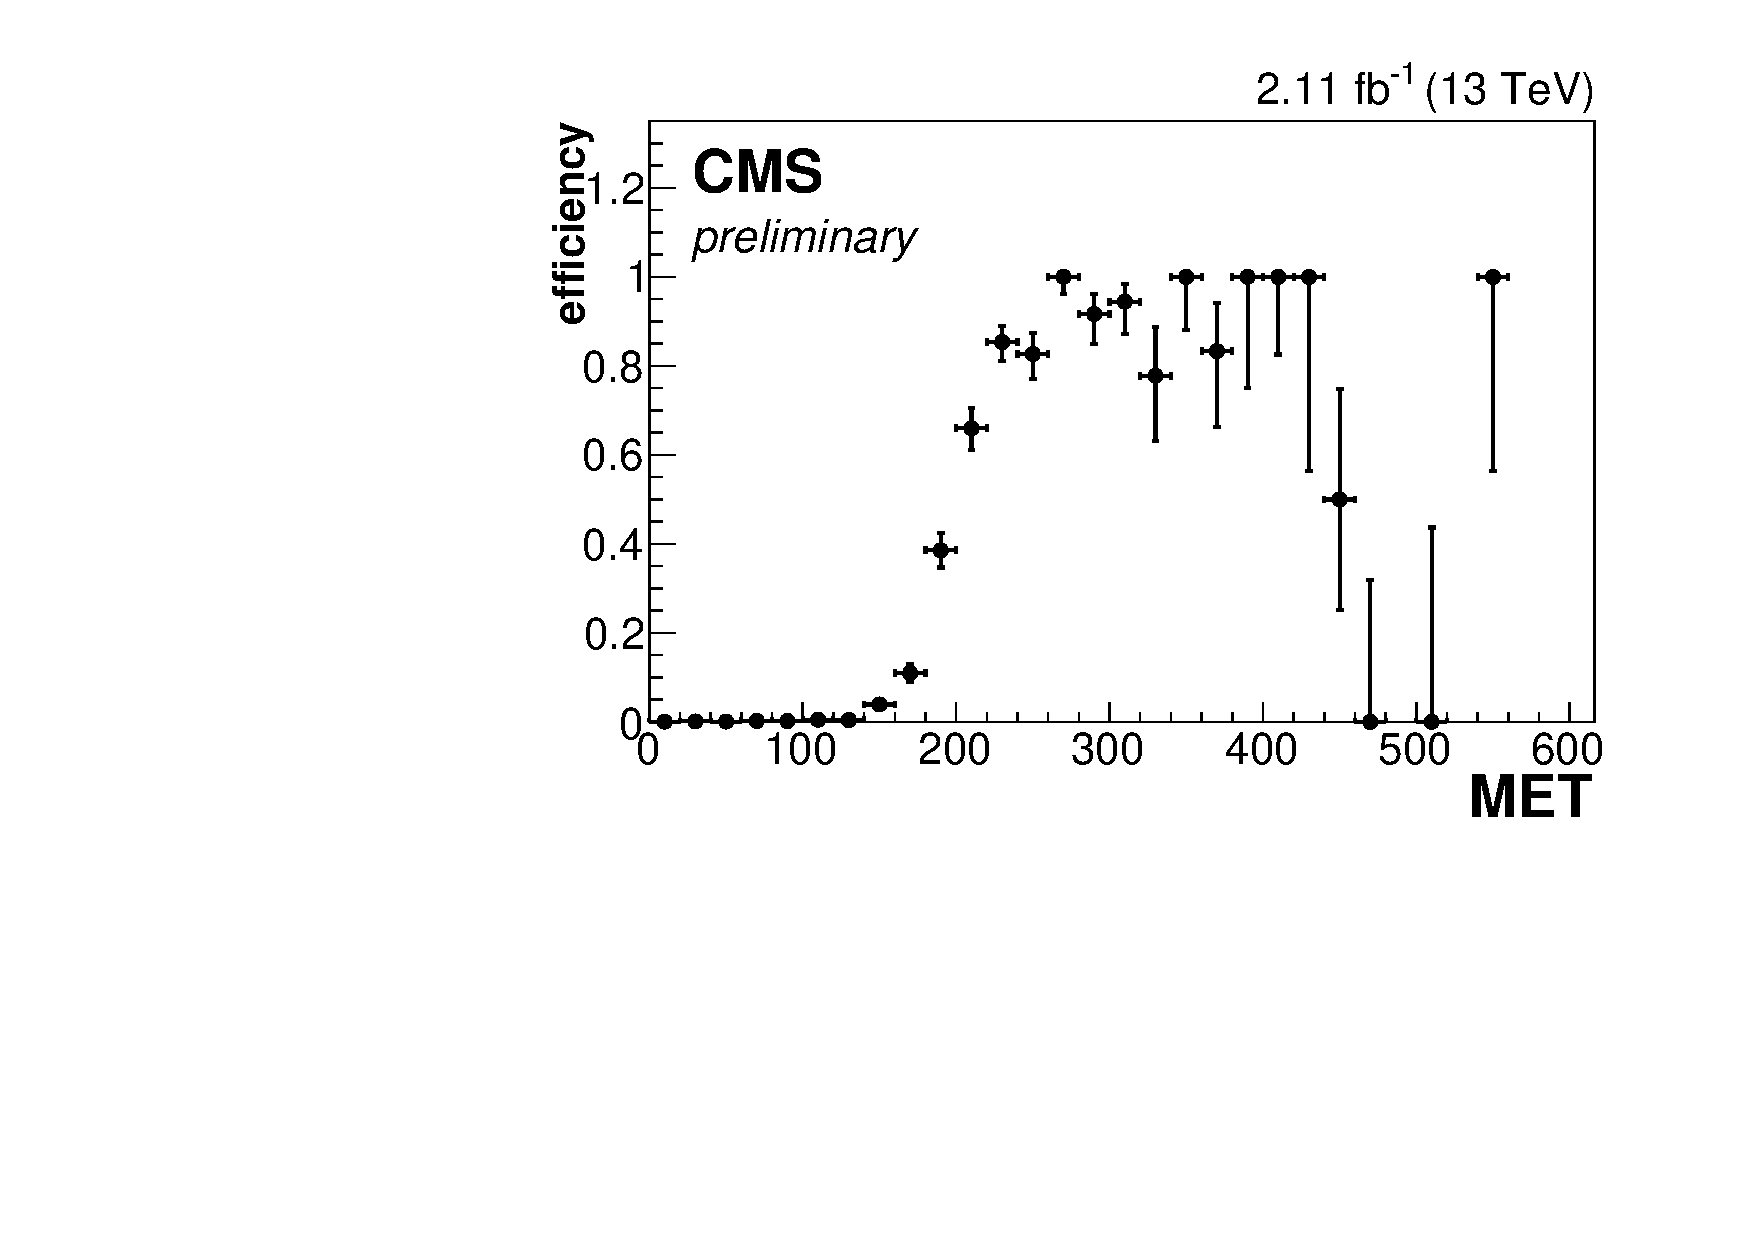
\includegraphics[width=.5\textwidth]{TalkPics/trigeff301115/output_2015Dtrigeff_131115json_mettrigger_vbfphasespaceAM_301115/nunu_met.pdf}
  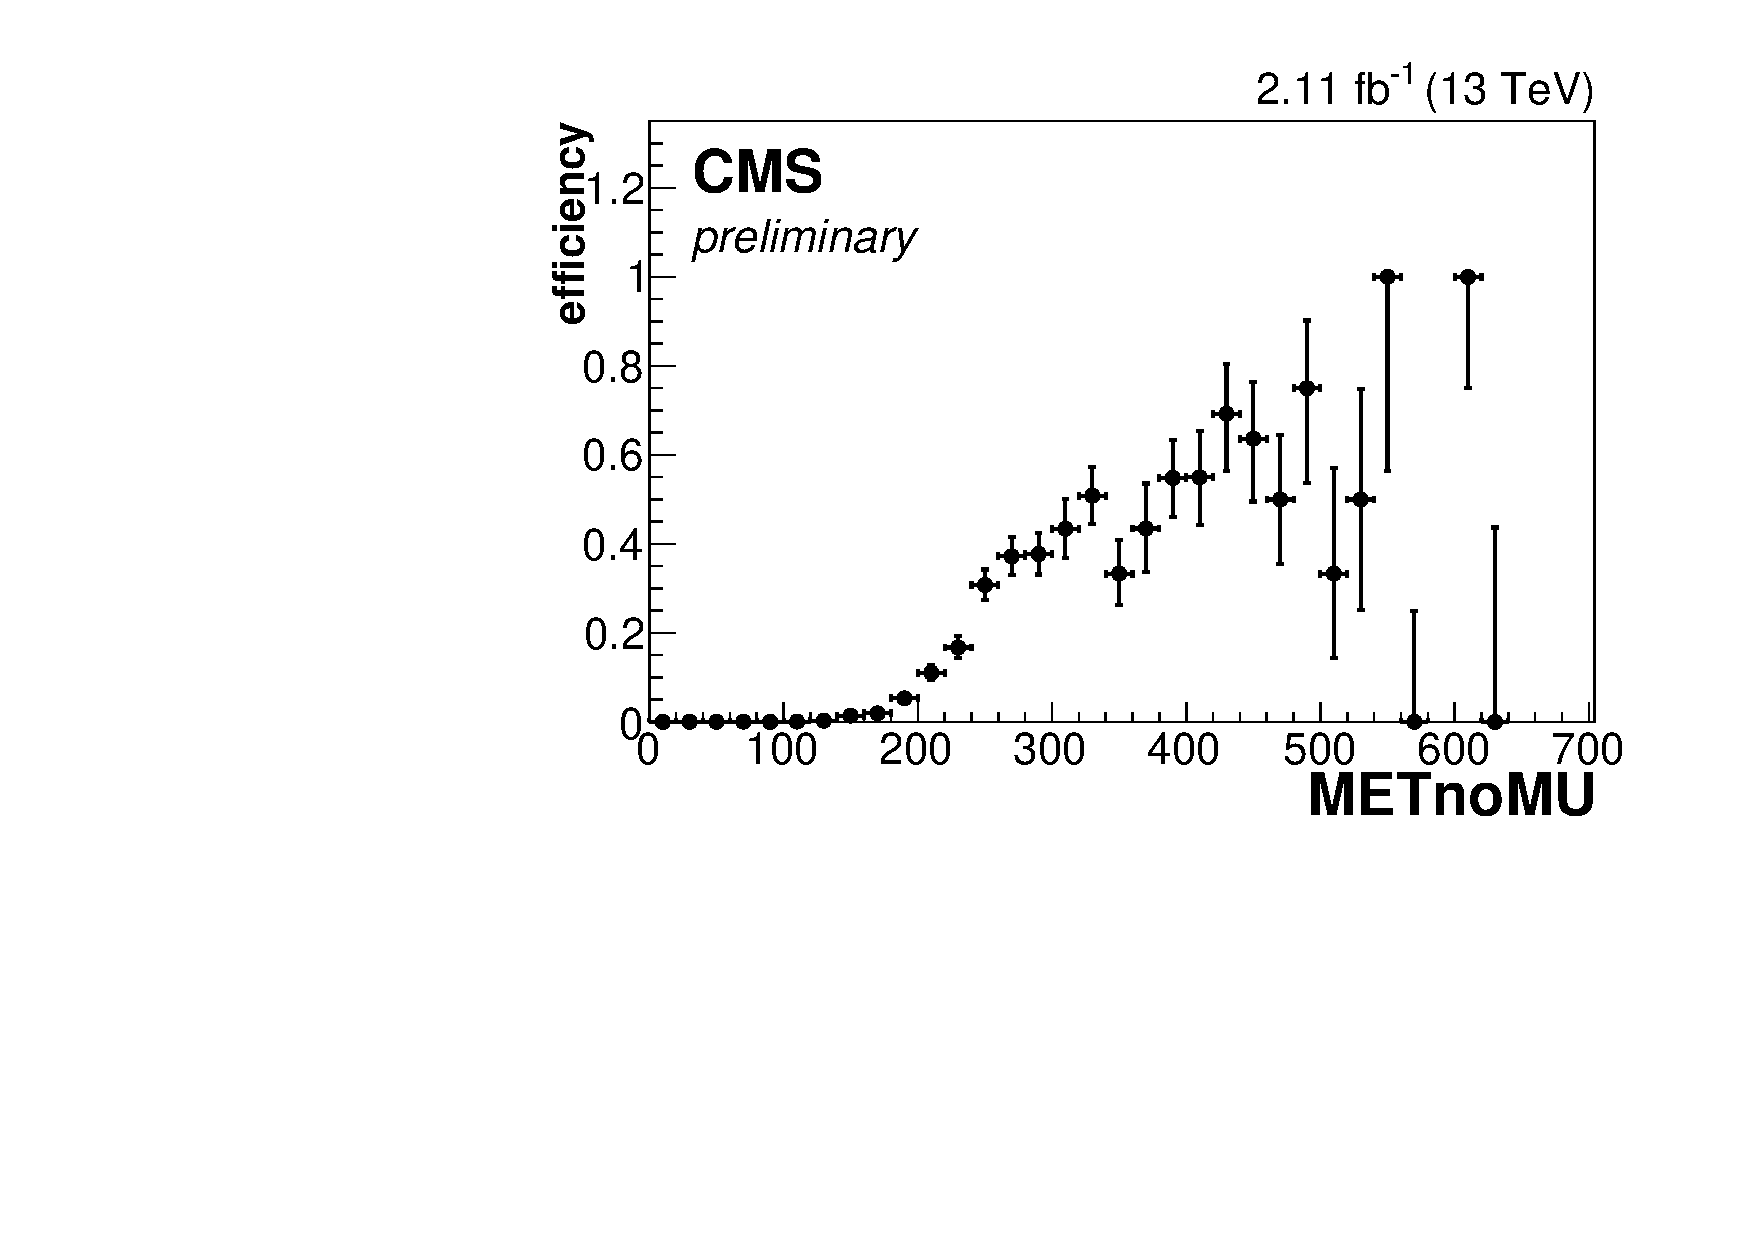
\includegraphics[width=.5\textwidth]{TalkPics/trigeff301115/output_2015Dtrigeff_131115json_mettrigger_vbfphasespaceAM_301115/nunu_metnomuons.pdf}
\end{frame}

\begin{frame}
  \frametitle{Summary of Studies}
  \scriptsize
  \vspace{-.2cm}
  \begin{block}{}
    \begin{itemize}
    \item L1ETM60 is inefficient in the VBF phase space due to it ignoring the HF
    \item[-] We lose signal from this L1 inefficiency
    \item[-] Variable correlation makes denominator cuts high, looks worse for softer events
    \item[-] Even after factoring out L1 effect still less efficient than in run 1, especially jet pt
    \item Incorrect JEC was used in HLT during Run2015
    \item[-] Calo jet JEC are large so this could cause problems
    \item[-] Calo jets with 30 GeV $p_{T}$ frequently have offline $p_{T}$ above pf trigger threshold
    \item[-] HLT efficiency is better in MC than data
    \item[-] Suggests wrong JEC could be to blame
    \item[-] Reemulating trigger on raw data so we can check if events failing trigger fail calo filter or pf filter
    \item Signal trigger still provides much better efficiency for control regions than MET only trigger
    \item Efficiency next year expected to be much improved by better JEC and possible L1MET including HF
    \end{itemize}
  \end{block}
  \centering
\end{frame}

\begin{frame}
  \frametitle{Plots for Approval Tomorrow}
  \scriptsize
  \vspace{-.3cm}
  \begin{block}{}
    \begin{itemize}
    \item Left caption: Efficiency of VBF Higgs to invisible trigger in data as a function of MET ignoring muons (METnoMU). The denominator of the efficiency is the number of events passing a single muon trigger which have two jets with $p_{T}>80$ GeV, $M_{jj}>600$ GeV and $\Delta\eta_{jj}>3.6$ GeV.
    \item Right caption: Efficiency of VBF Higgs to invisible trigger in data as a function of sub-leading jet $p_{T}$. The denominator of the efficiency is the number of events passing a single muon trigger which have a leading jet with $p_{t}>80$ GeV, $METnoMU>300$ GeV, $M_{jj}>600$ GeV and $\Delta\eta_{jj}>3.6$ GeV.

    \end{itemize}
  \end{block}
  \vspace{-.1cm}
  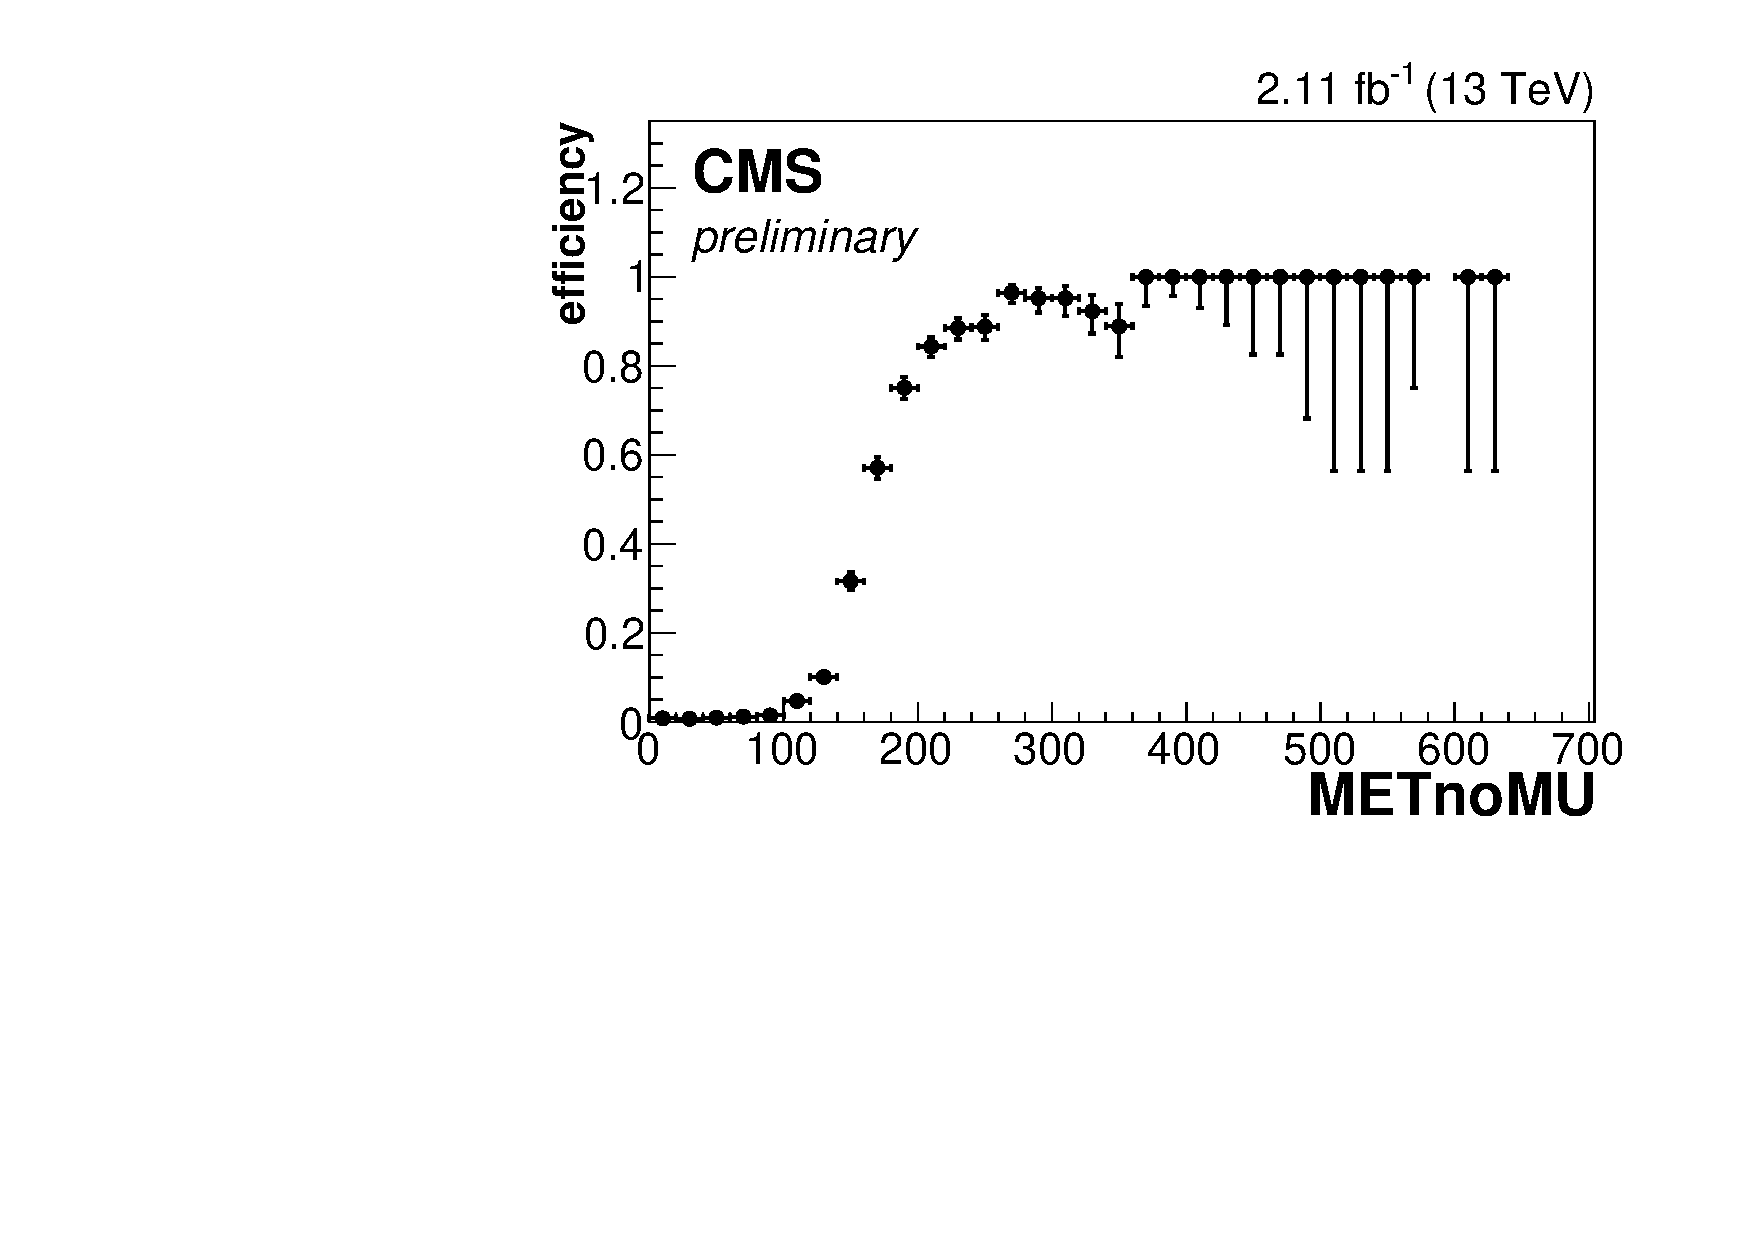
\includegraphics[width=0.5\textwidth]{TalkPics/trigeff301115/output_2015Dtrigeff_131115json_sigtrig_301115/nunu_metnomuons.pdf}
  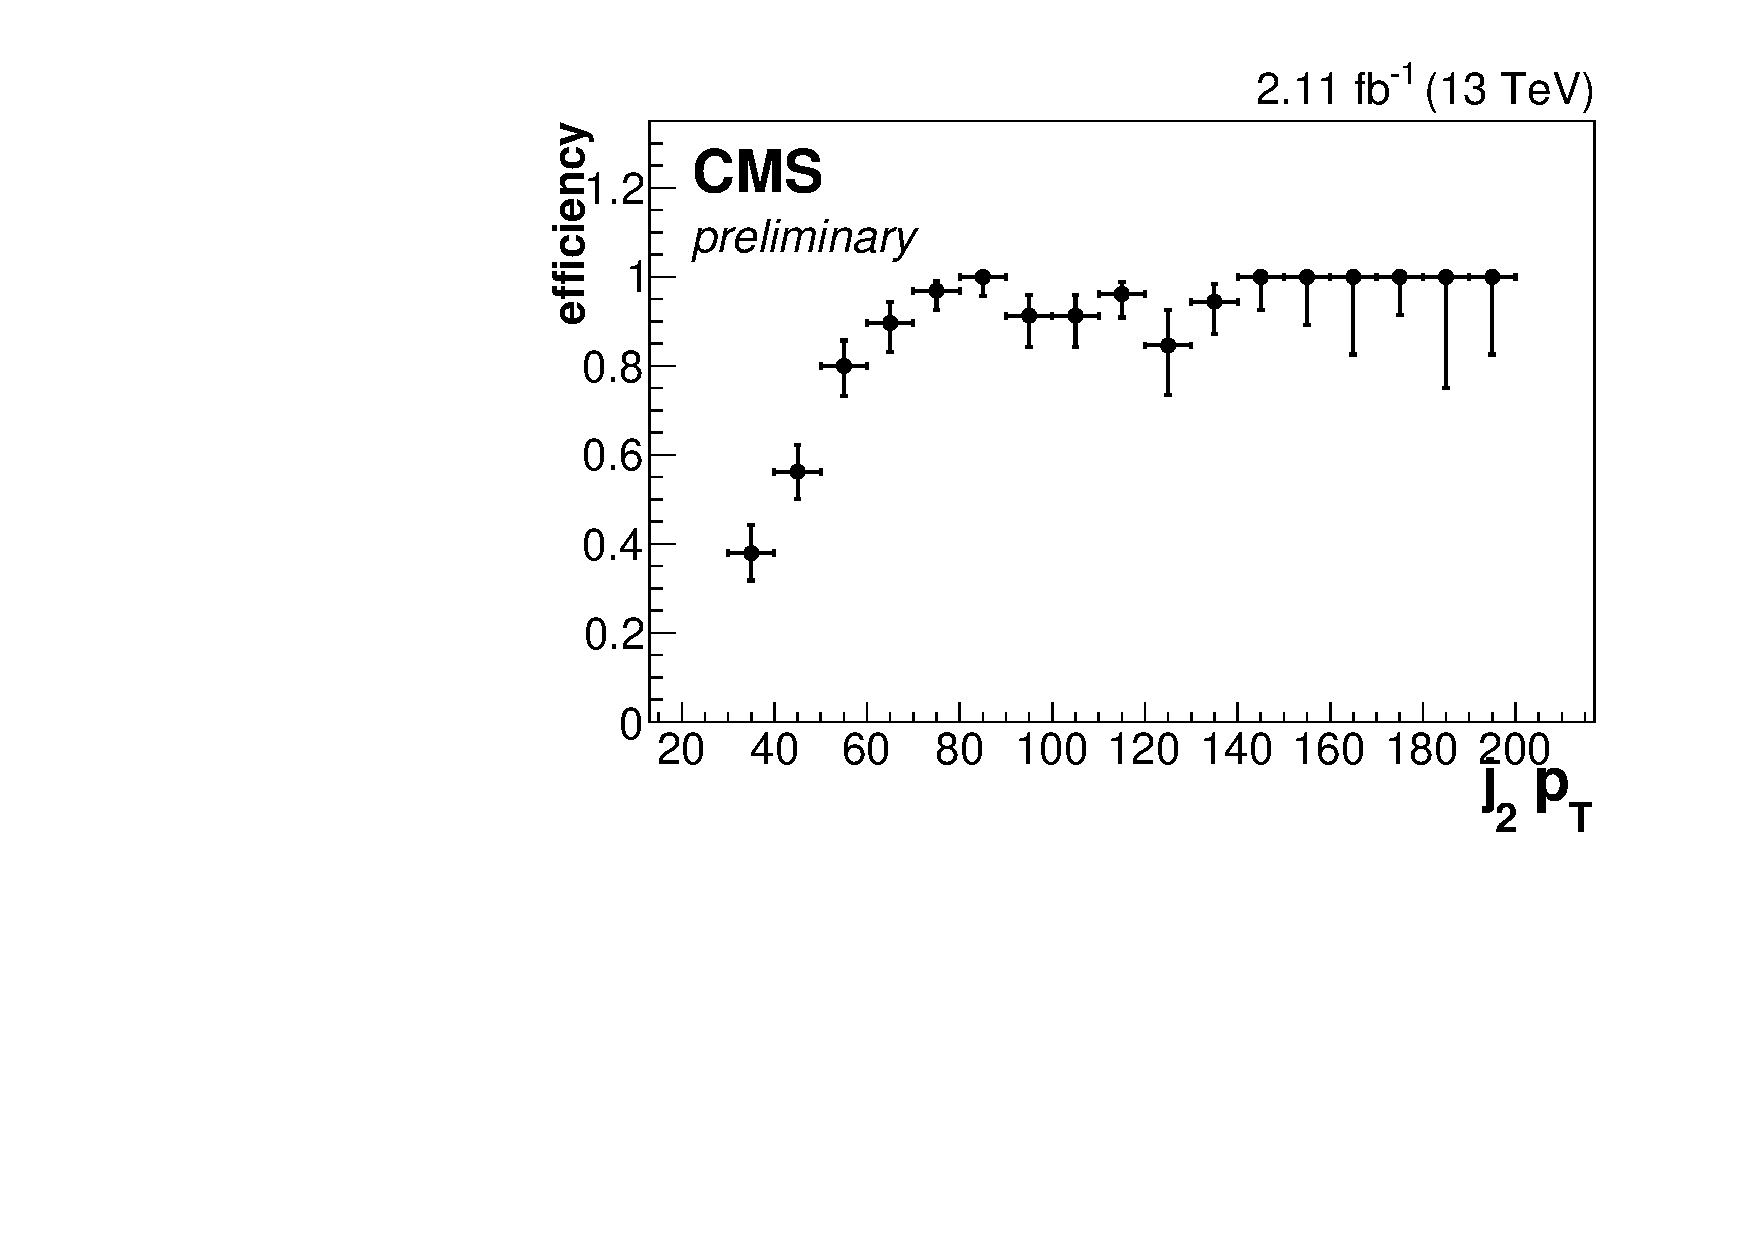
\includegraphics[width=0.5\textwidth]{TalkPics/trigeff301115/output_2015Dtrigeff_131115json_sigtrig_301115/nunu_jet2_pt.pdf}
\end{frame}

\begin{frame}
  \frametitle{Plots for Approval Tomorrow}
  \scriptsize
  \vspace{-.3cm}
  \begin{block}{}
    \begin{itemize}
    \item Left caption: Efficiency of VBF Higgs to invisible trigger in data as a function of dijet mass ($M_{jj}$). The denominator of the efficiency is the number of events passing a single muon trigger which have two jets with $p_{T}>80$ GeV, $METnoMU>300$ GeV and $\Delta\eta_{jj}>3.6$ GeV.
    \item Right caption: Efficiency of VBF Higgs to invisible trigger in data as a function of dijet $\Delta\eta$. The denominator of the efficiency is the number of events passing a single muon trigger which have two jets with $p_{T}>80$ GeV, $METnoMU>300$ GeV and $M_{jj}>600$ GeV.
    \end{itemize}
  \end{block}
  \vspace{-.1cm}
  \includegraphics[width=0.5\textwidth]{TalkPics/trigeff301115/output_2015Dtrigeff_131115json_sigtrig_301115/nunu_dijet_M.pdf}
  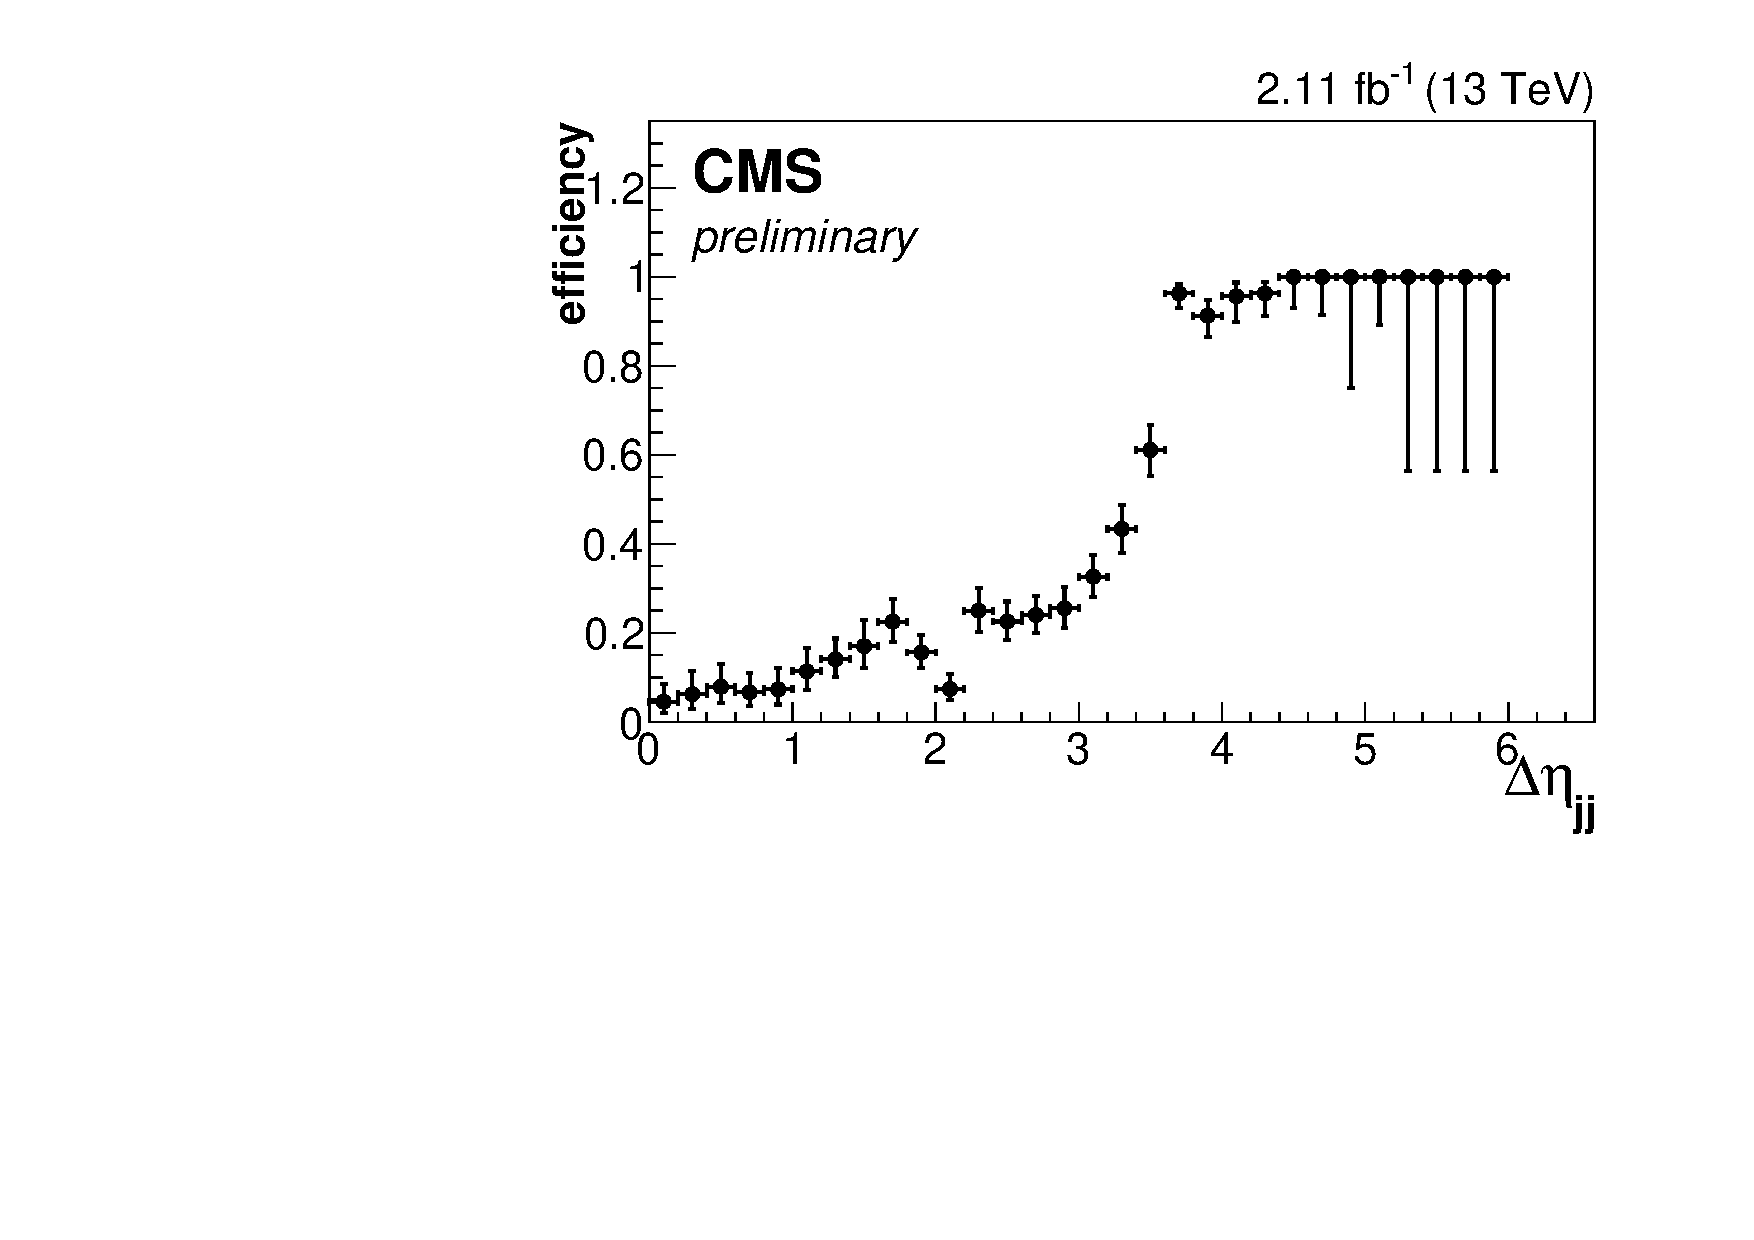
\includegraphics[width=0.5\textwidth]{TalkPics/trigeff301115/output_2015Dtrigeff_131115json_sigtrig_301115/nunu_dijet_deta.pdf}
\end{frame}

\begin{frame}
  \frametitle{Plots for Approval Tomorrow}
  \scriptsize
  \vspace{-.2cm}
  \begin{columns}
    \column{1.1\textwidth}
  \begin{block}{}
    \begin{itemize}
    \item Left caption: Efficiency of MET only trigger in data as a function of MET. The denominator of the efficiency is the number of events passing a single muon trigger which have two jets with $p_{T}>50$ GeV, $M_{jj}>800$ GeV and $\Delta\eta_{jj}>3.6$ GeV.
    \item Right caption: Efficiency of MET only trigger in data as a function of MET ignoring muons (METnoMU). The denominator of the efficiency is the number of events passing a single muon trigger which have two jets with $p_{T}>50$ GeV, $M_{jj}>800$ GeV and $\Delta\eta_{jj}>3.6$ GeV.
    \end{itemize}
  \end{block}
  \end{columns}
  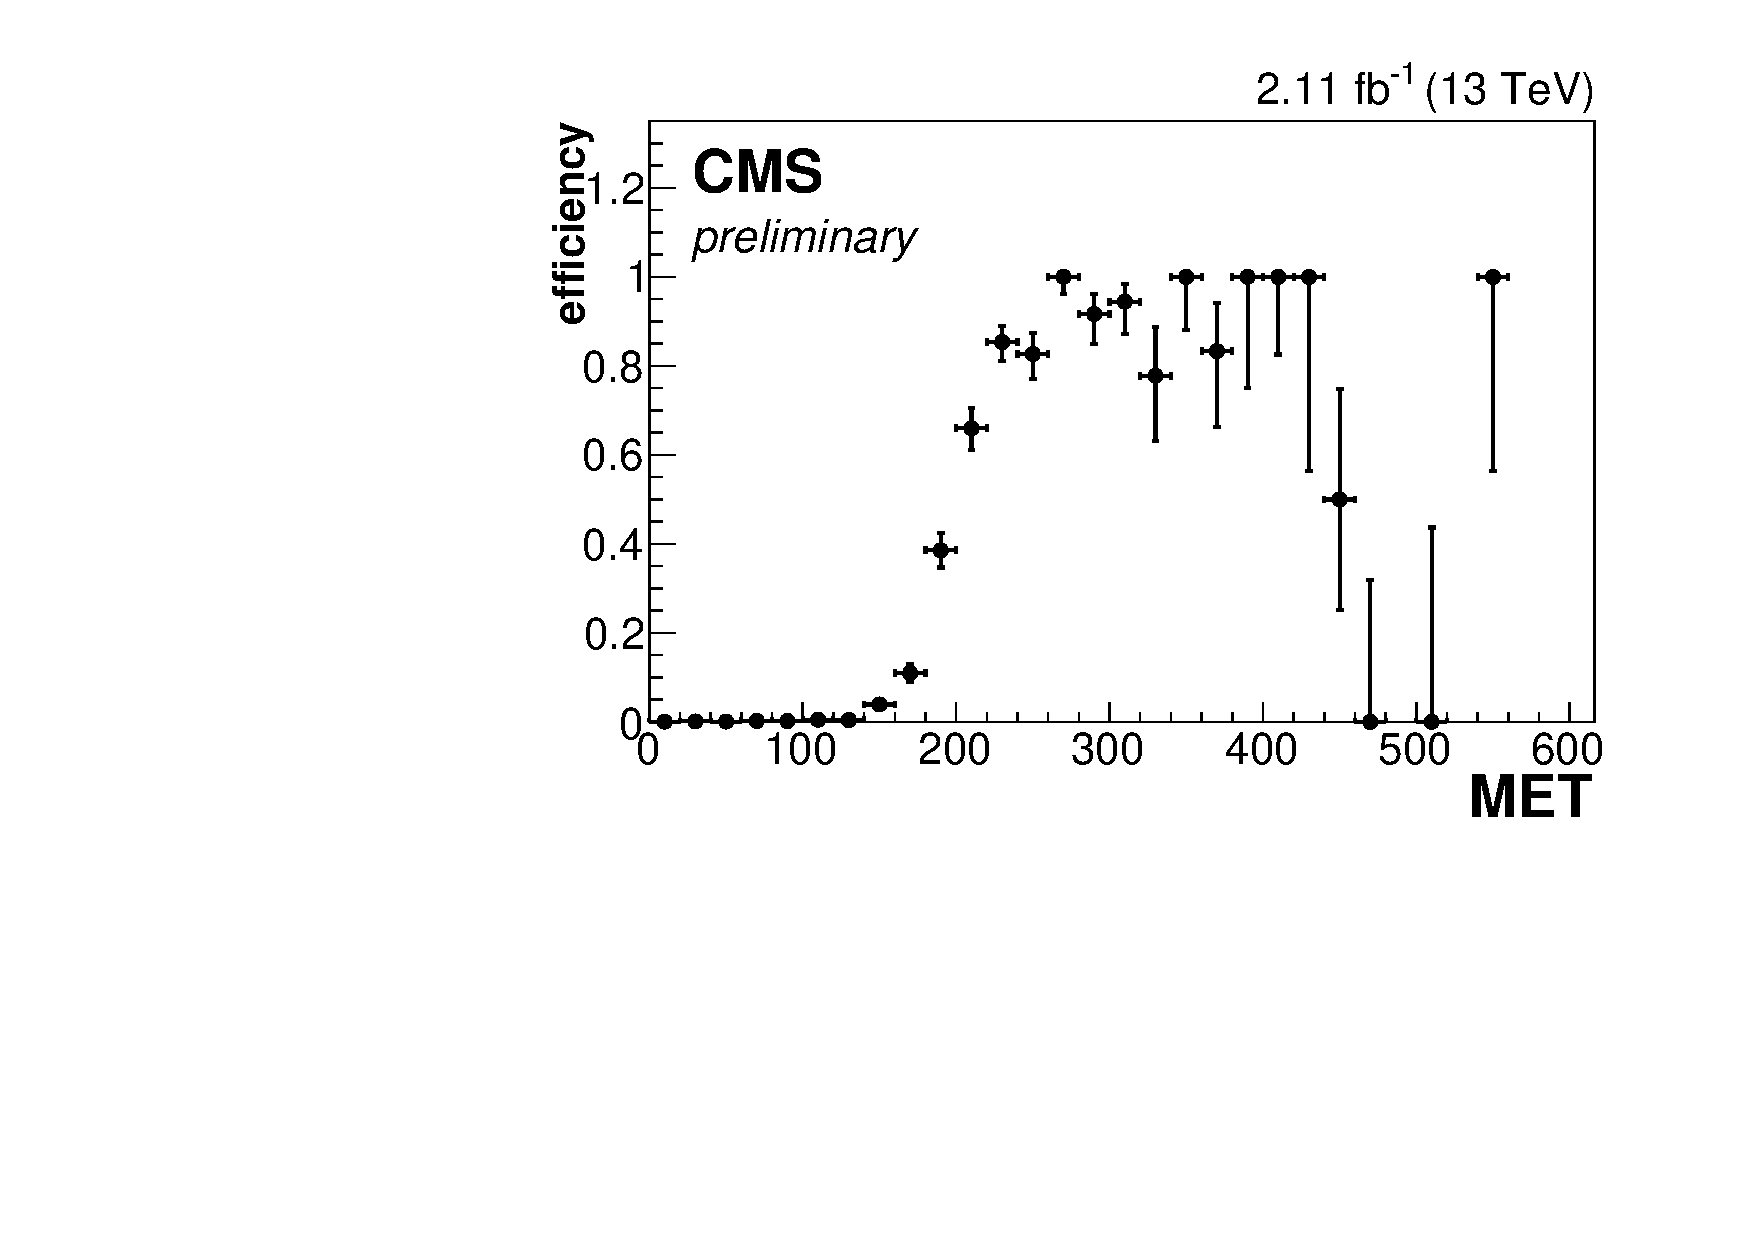
\includegraphics[width=.5\textwidth]{TalkPics/trigeff301115/output_2015Dtrigeff_131115json_mettrigger_vbfphasespaceAM_301115/nunu_met.pdf}
  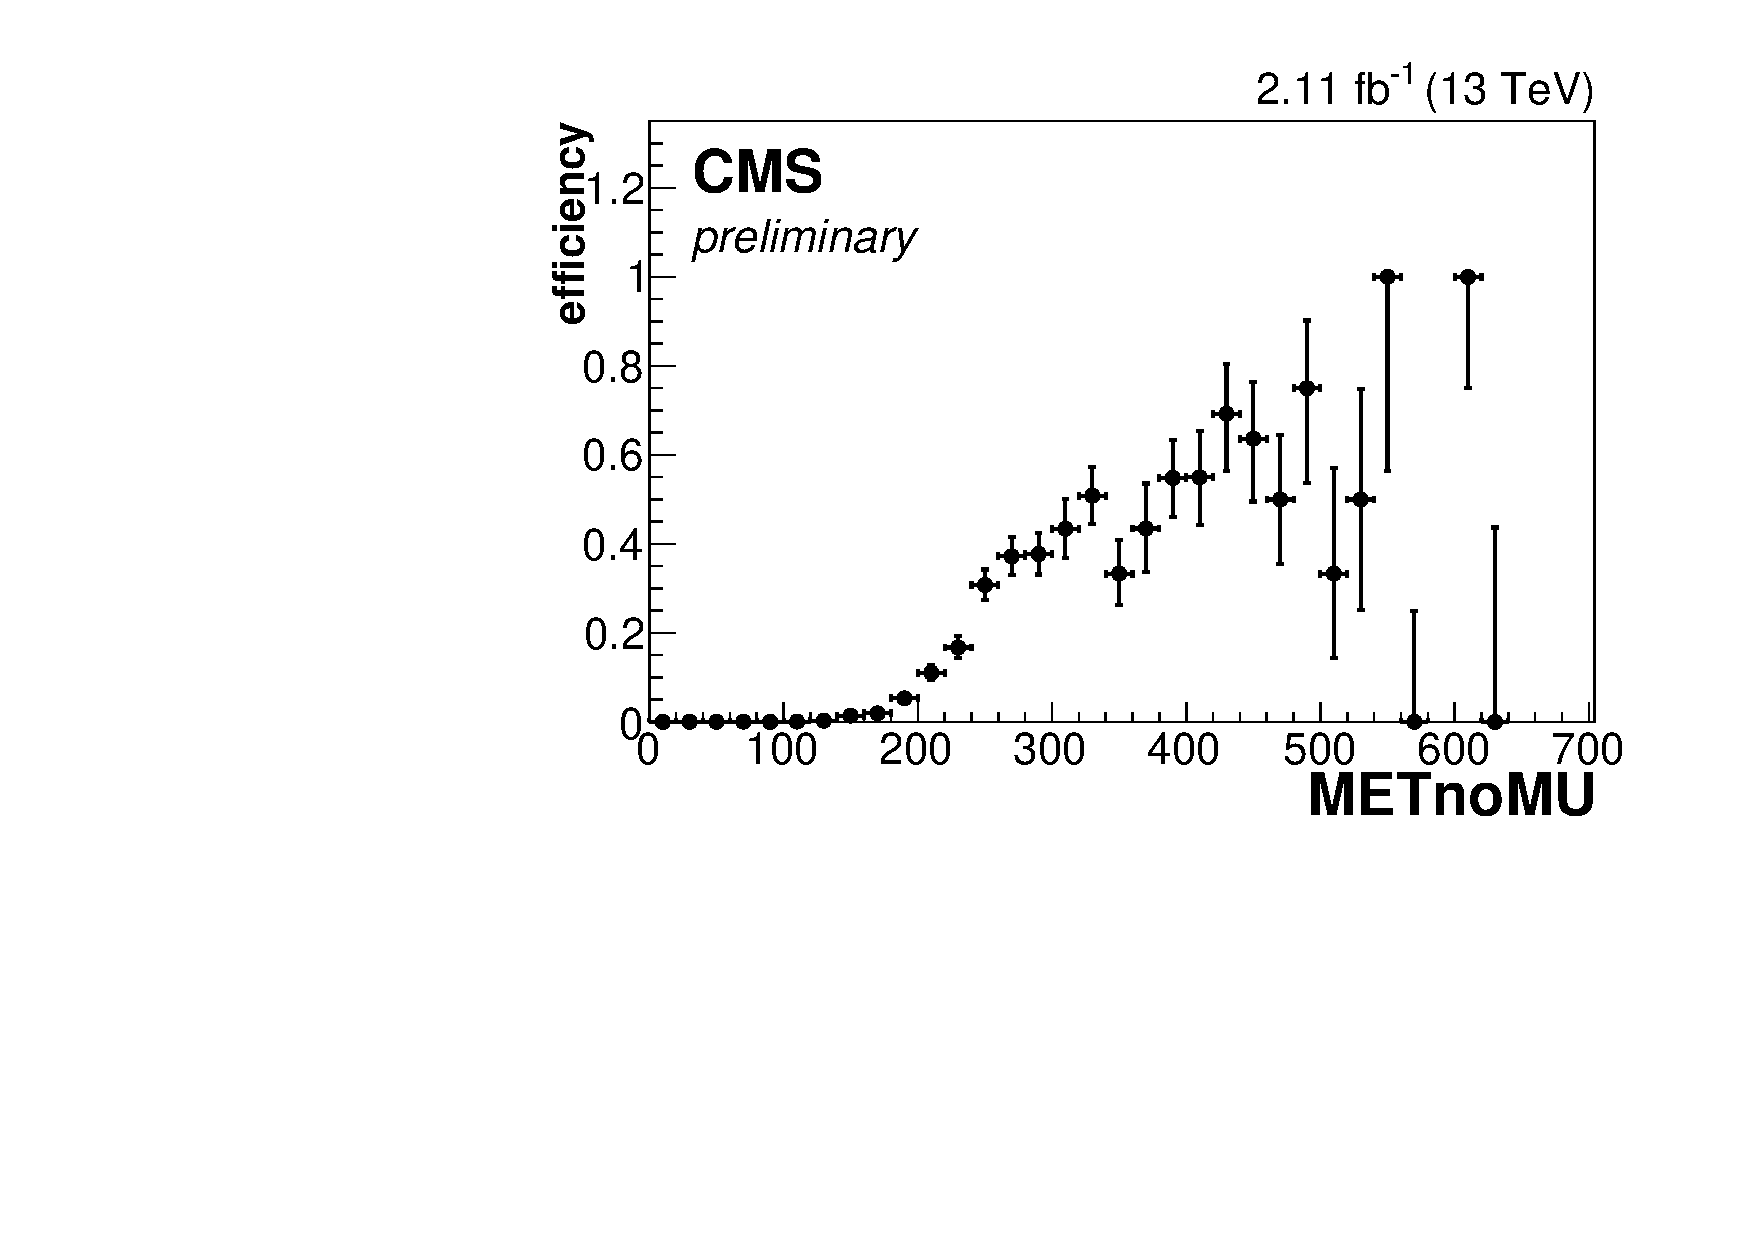
\includegraphics[width=.5\textwidth]{TalkPics/trigeff301115/output_2015Dtrigeff_131115json_mettrigger_vbfphasespaceAM_301115/nunu_metnomuons.pdf}
\end{frame}

\begin{frame}
  \frametitle{Plots for Approval Tomorrow}
  \scriptsize
  \centering
  \begin{block}{}
    \begin{itemize}
    \item Caption: The Level 1 (black), HLT (red) and total (blue) efficiency of the VBF Higgs to invisible trigger in MC as a function of MET ignoring muons (METnoMU). The denominator of the efficiency is the number of events in a signal MC sample which have two jets with $p_{T}>80$ GeV, $M_{jj}>600$ GeV and $\Delta\eta_{jj}>3.6$ GeV.

    \end{itemize}
  \end{block}
  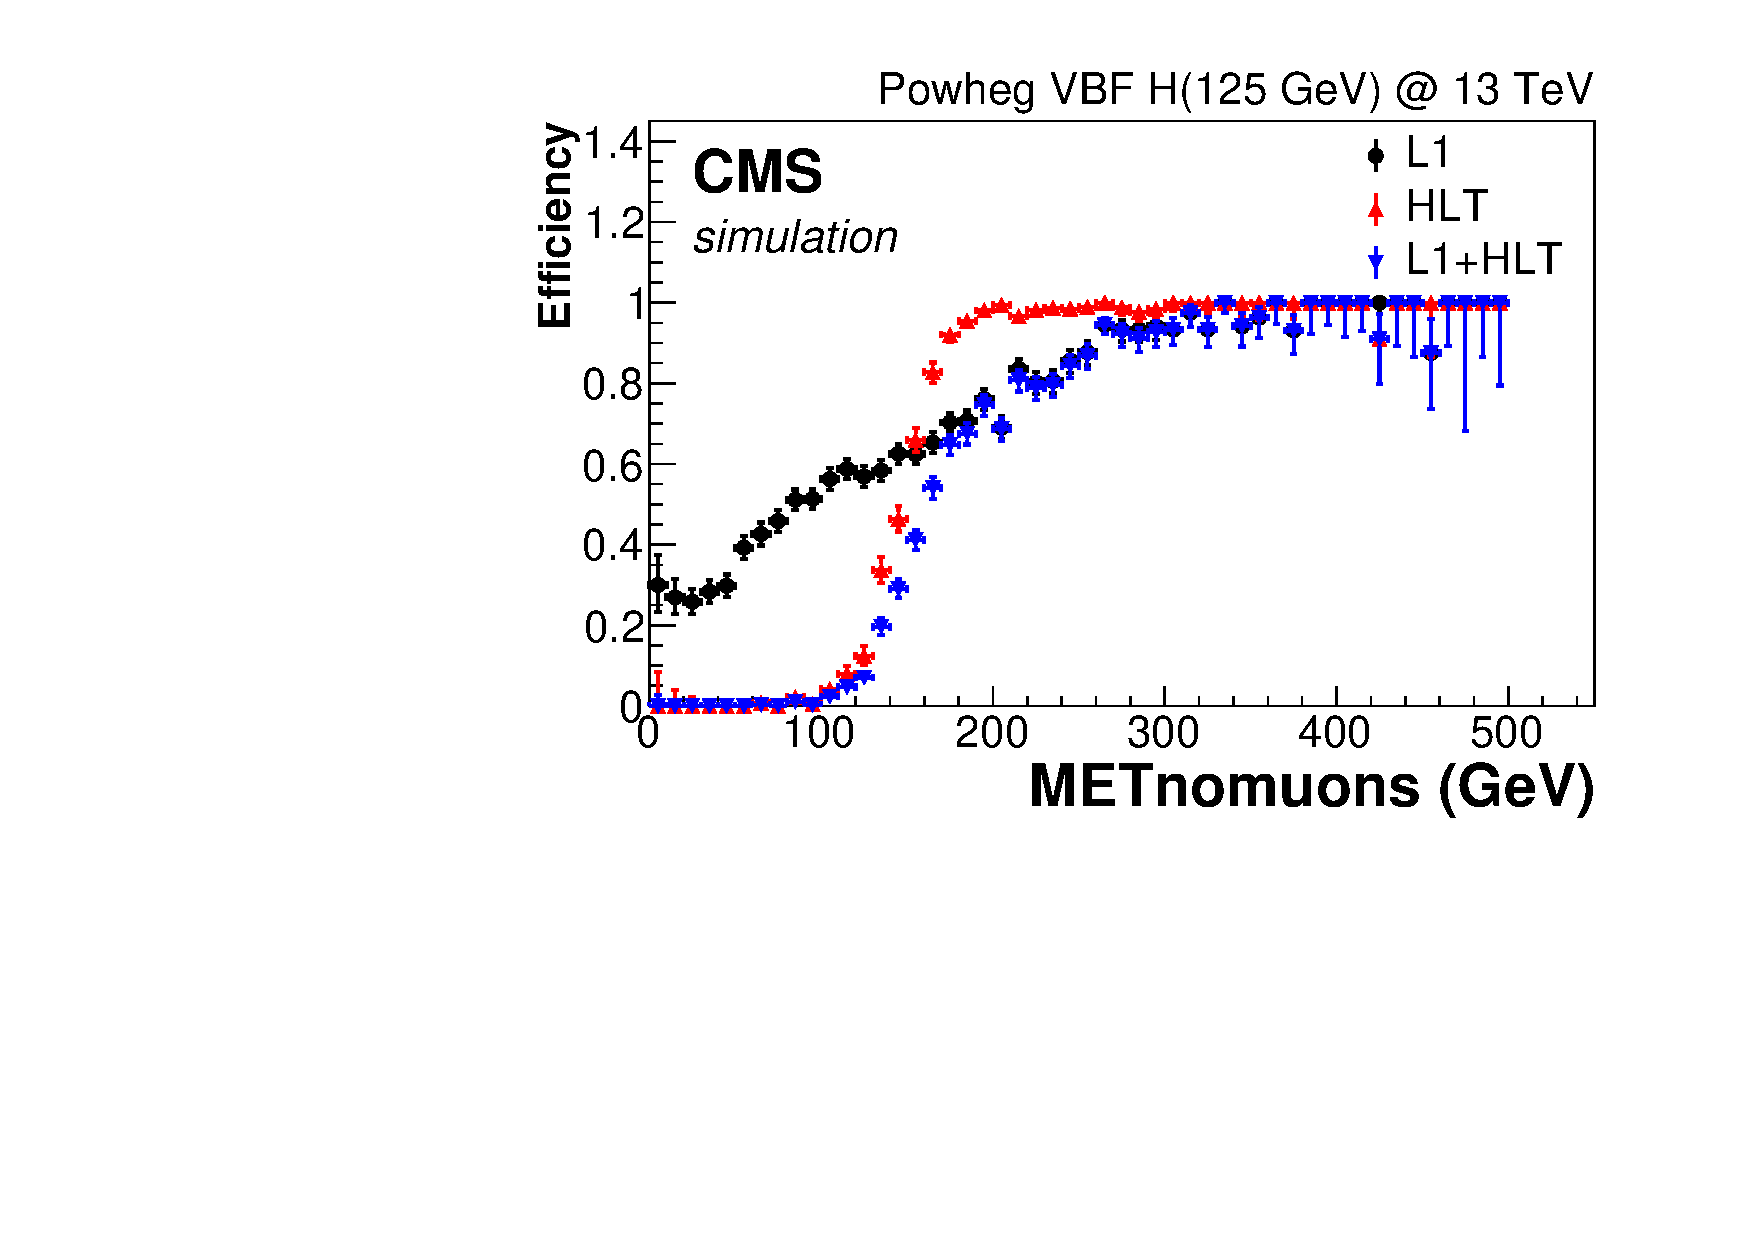
\includegraphics[width=.5\textwidth]{TalkPics/trigeff301115/SigTrigEff_metnomuons.pdf}
\end{frame}

\begin{frame}
  \frametitle{Plots for Approval Tomorrow}
  \scriptsize
  \centering
  \begin{block}{}
    \begin{itemize}
    \item Caption: The Level 1 (black), HLT (red) and total (blue) efficiency of the VBF Higgs to invisible trigger in MC as a function of sub-leading jet $p_{T}$. The denominator of the efficiency is the number of events passing in a signal MC sample which have a leading jet with $p_{t}>80$ GeV, $METnoMU>300$ GeV, $M_{jj}>600$ GeV and $\Delta\eta_{jj}>3.6$ GeV.

    \end{itemize}
  \end{block}
  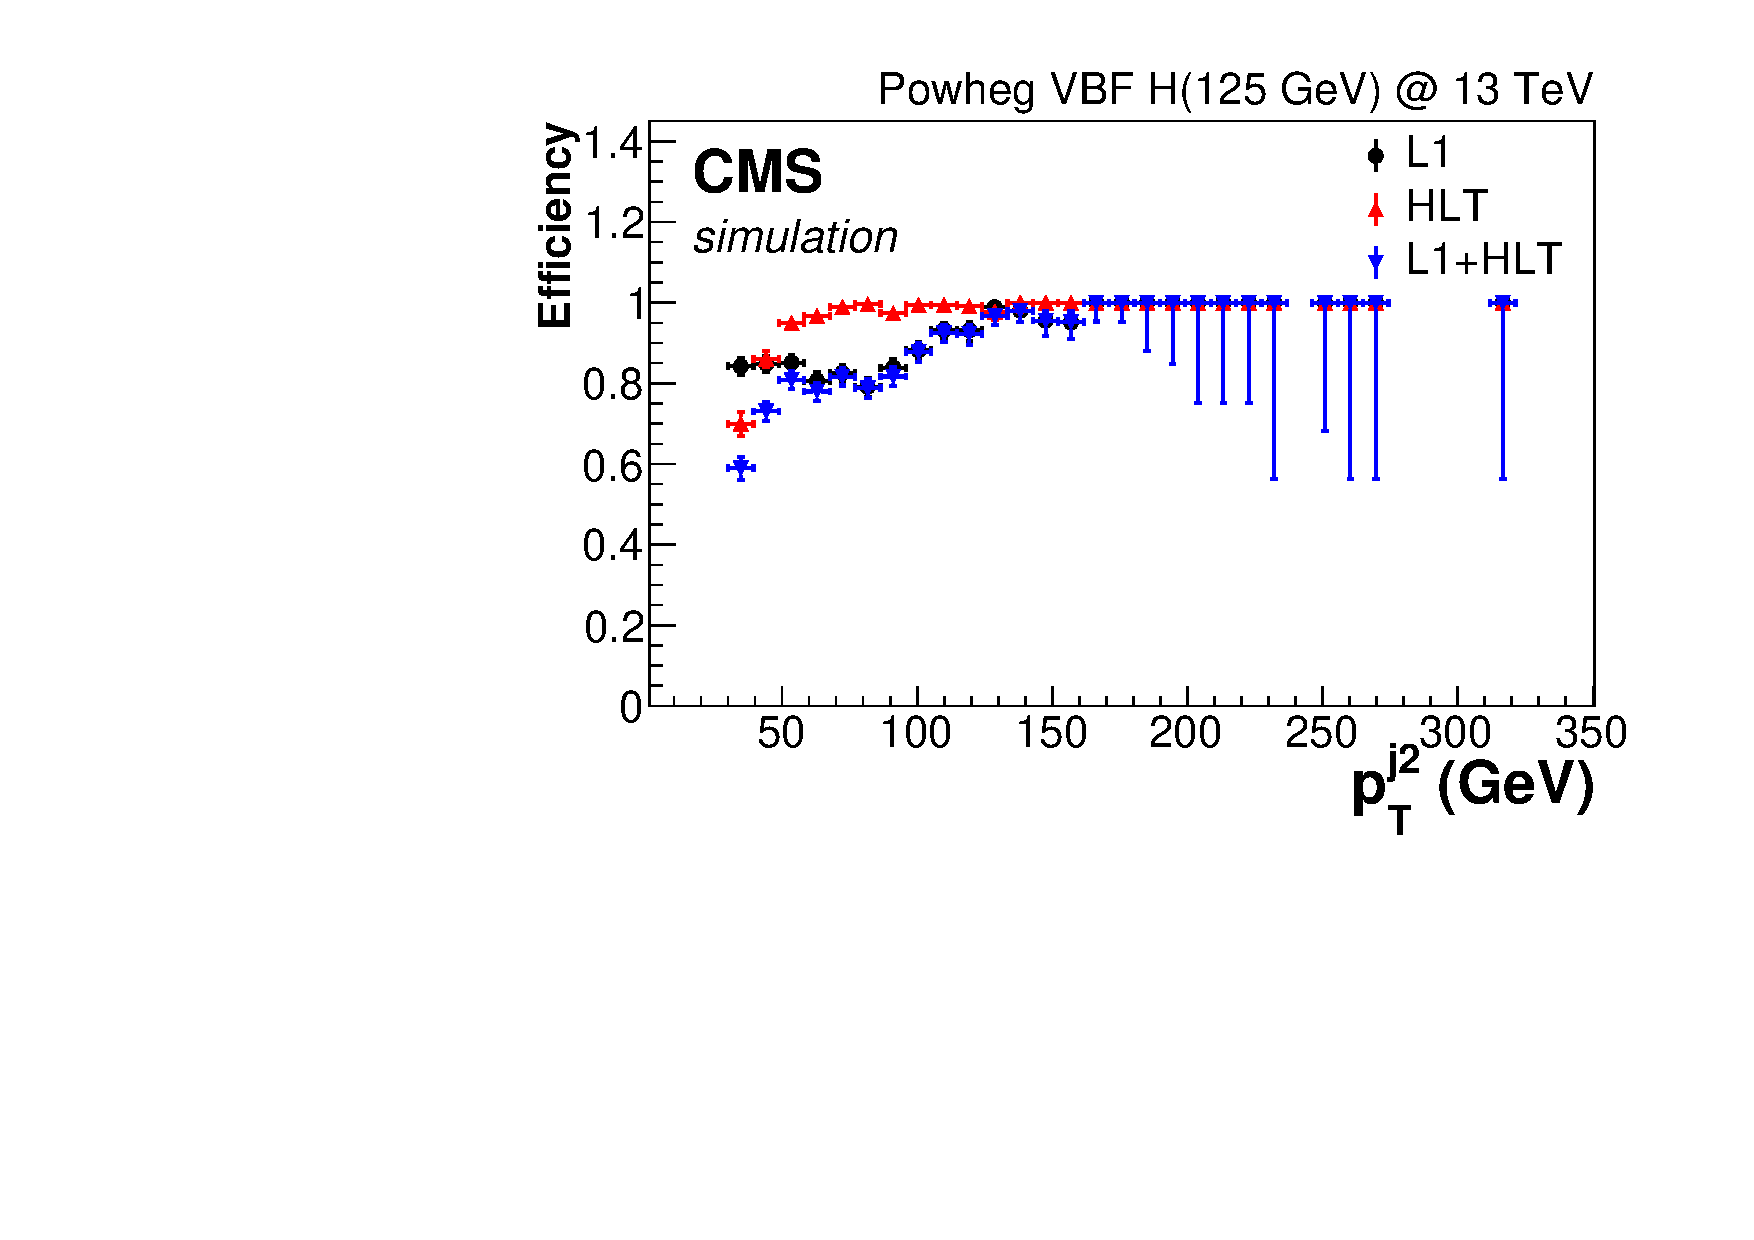
\includegraphics[width=.5\textwidth]{TalkPics/trigeff301115/SigTrigEff_jet2_pt.pdf}
\end{frame}

\begin{frame}
  \frametitle{Plots for Approval Tomorrow}
  \scriptsize
  \centering
  \begin{block}{}
    \begin{itemize}
    \item Caption: The Level 1 (black), HLT (red) and total (blue) efficiency of the VBF Higgs to invisible trigger in MC as a function of dijet mass ($M_{jj}$). The denominator of the efficiency is the number of events passing a signal MC sample which have two jets with $p_{T}>80$ GeV, $METnoMU>300$ GeV and $\Delta\eta_{jj}>3.6$ GeV.
    \end{itemize}
  \end{block}
  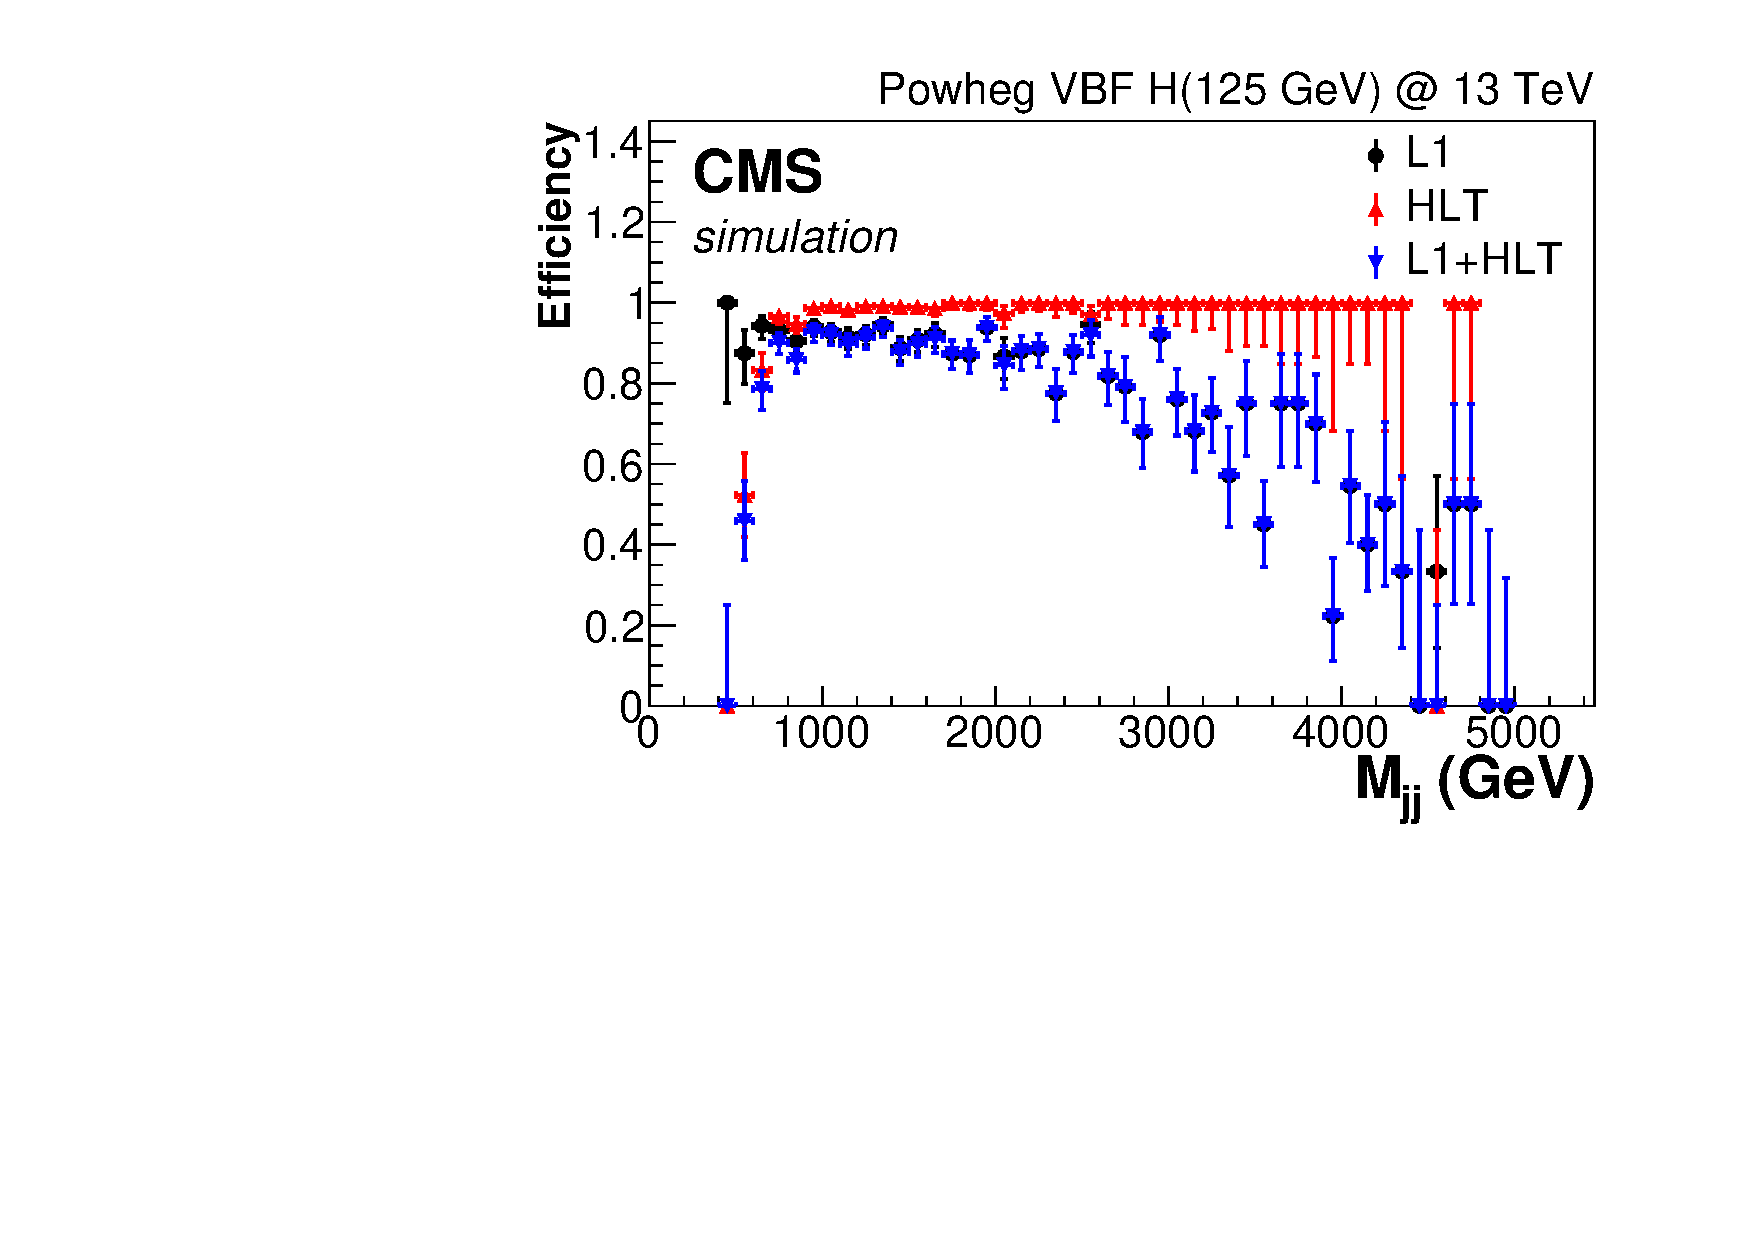
\includegraphics[width=.5\textwidth]{TalkPics/trigeff301115/SigTrigEff_dijet_M.pdf}
\end{frame}

\begin{frame}
  \frametitle{Plots for Approval Tomorrow}
  \scriptsize
  \centering
  \begin{block}{}
    \begin{itemize}
    \item Caption: The Level 1 (black), HLT (red) and total (blue) efficiency of the VBF Higgs to invisible trigger in MC as a function of dijet $\Delta\eta$. The denominator of the efficiency is the number of events passing a signal MC sample which have two jets with $p_{T}>80$ GeV, $METnoMU>300$ GeV and $M_{jj}>600$ GeV.
    \end{itemize}
  \end{block}
  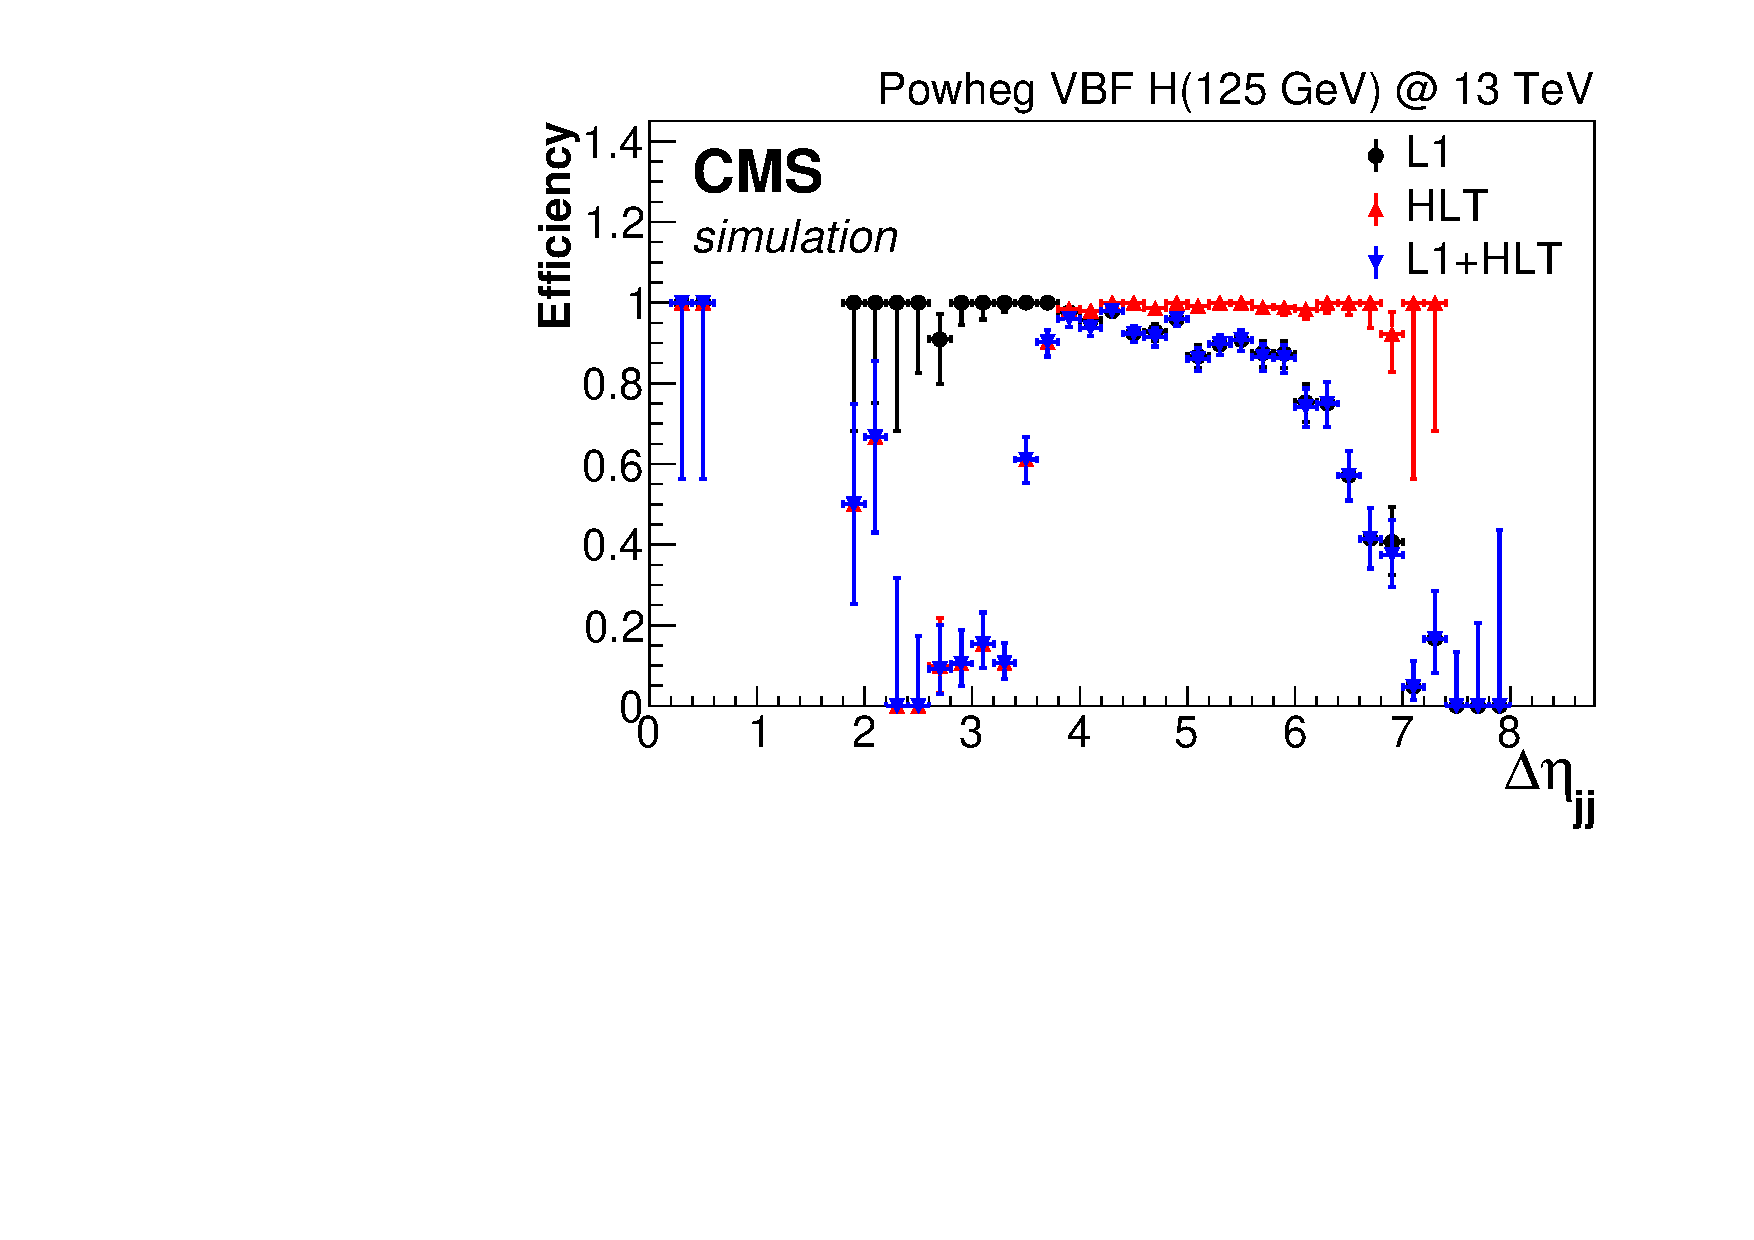
\includegraphics[width=.5\textwidth]{TalkPics/trigeff301115/SigTrigEff_dijet_deta.pdf}
\end{frame}

\begin{frame}
  \frametitle{Summary}
  \label{lastframe}
  \scriptsize
  \begin{block}{}
  \begin{itemize}
  \item We have a good understanding of our trigger turn ons
  \item[-] We see some inefficiencies due to L1 MET $\eta$ restriction and possible incorrect JEC effects
  \item We will ask tomorrow for approval to show the trigger turn on curves at the December jamboree
  \end{itemize}
  \end{block}
\end{frame}


%UPDATED BACKUP
\begin{frame}
  \frametitle{Backup}
\end{frame}

\begin{frame}
  \frametitle{$\Delta\eta_{jj}$ data turn on}
  \scriptsize
  \begin{block}{}
    \begin{itemize}
    \item Measure HLT efficiency (left) and L1+HLT efficiency (right)
    \item Dataset: Full 2015D data with latest JECv6
    \item Trigger: HLT\_DiPFJet40\_DEta3p5\_MJJ600\_PFMETNoMu140
    \item Denominator: SingleMuon events with dijet $p_{T}>80$, $M_{jj}>600$, $\Delta\eta_{jj}>3.6$ plus for left plot only L1ETM60
    \item Possible decrease at end of L1+HLT efficiency due to HF jets
    \end{itemize}
  \end{block}
  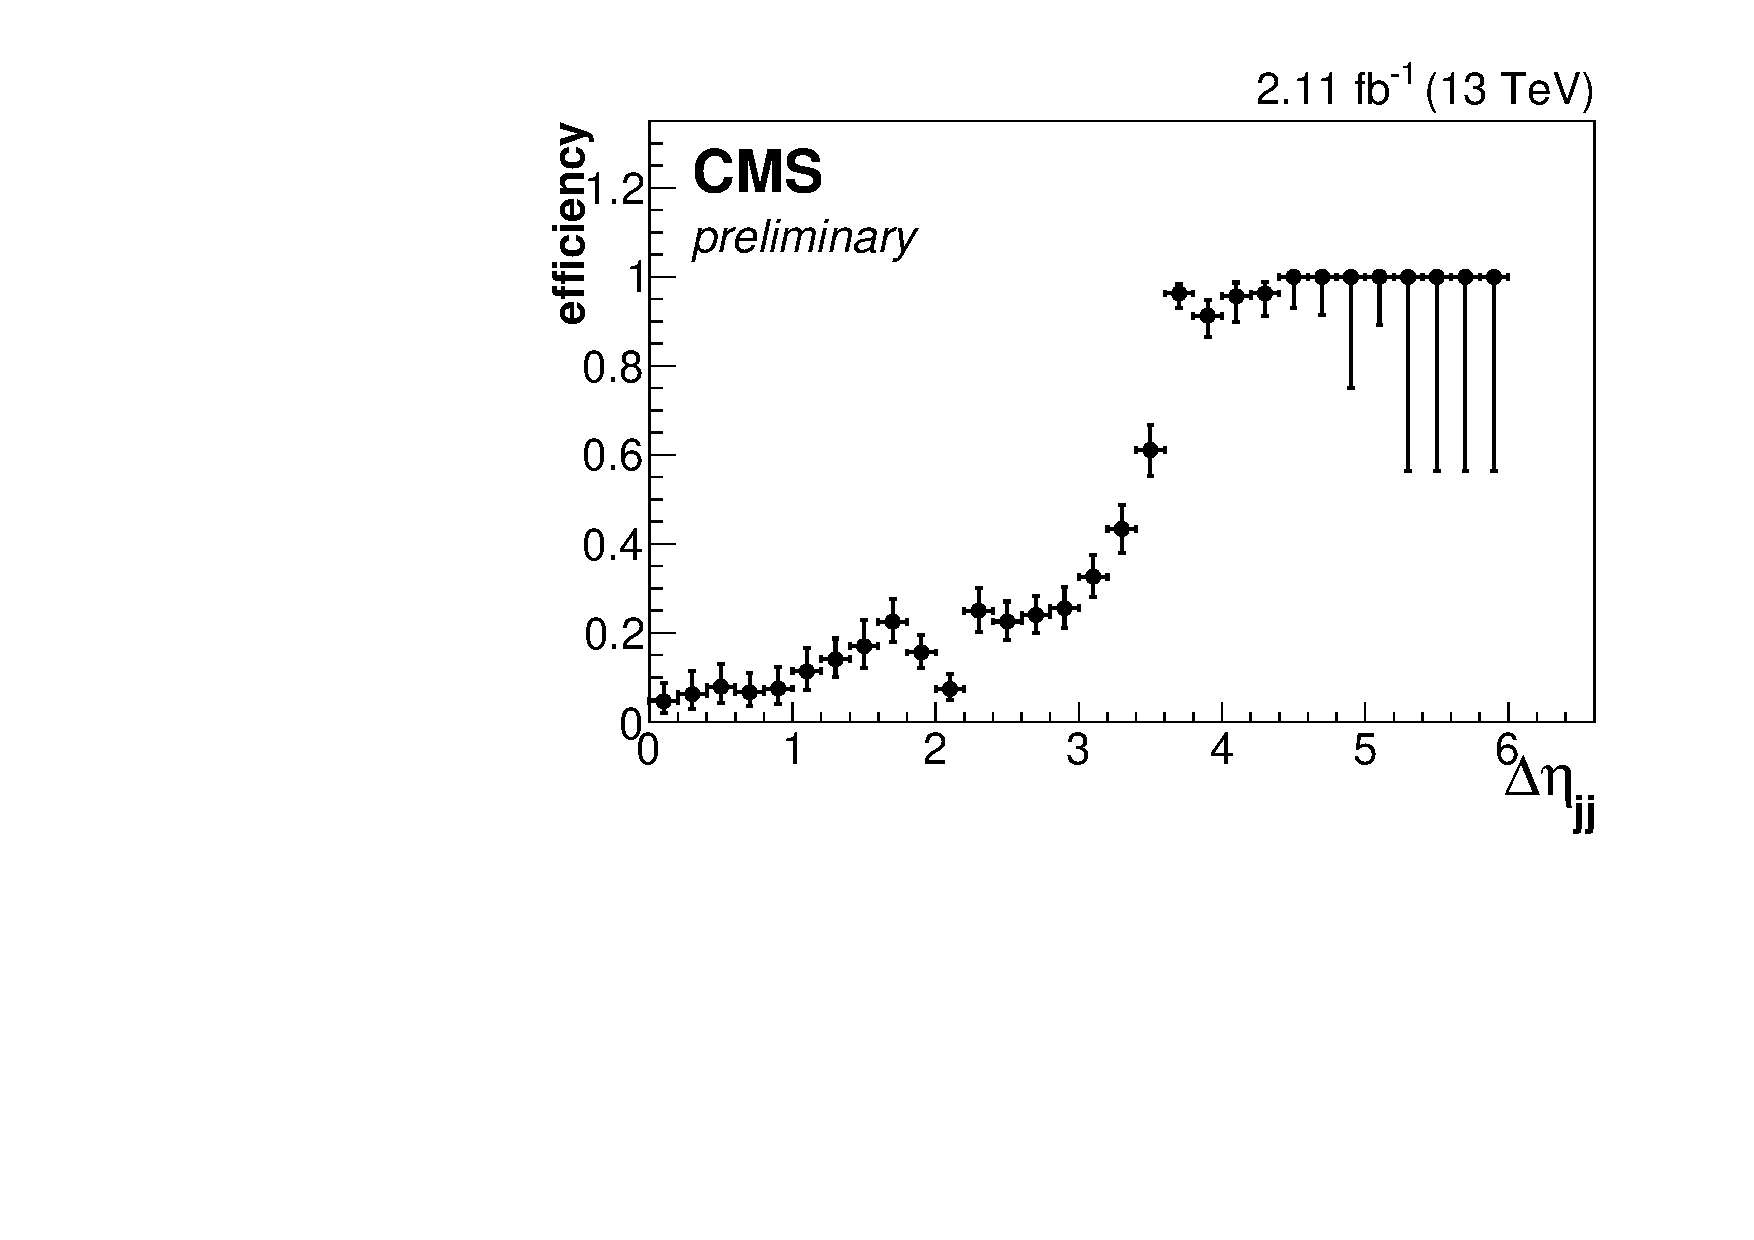
\includegraphics[width=.5\textwidth]{TalkPics/trigeff301115/output_2015Dtrigeff_131115json_sigtrig_hltonly_301115/nunu_dijet_deta.pdf}
  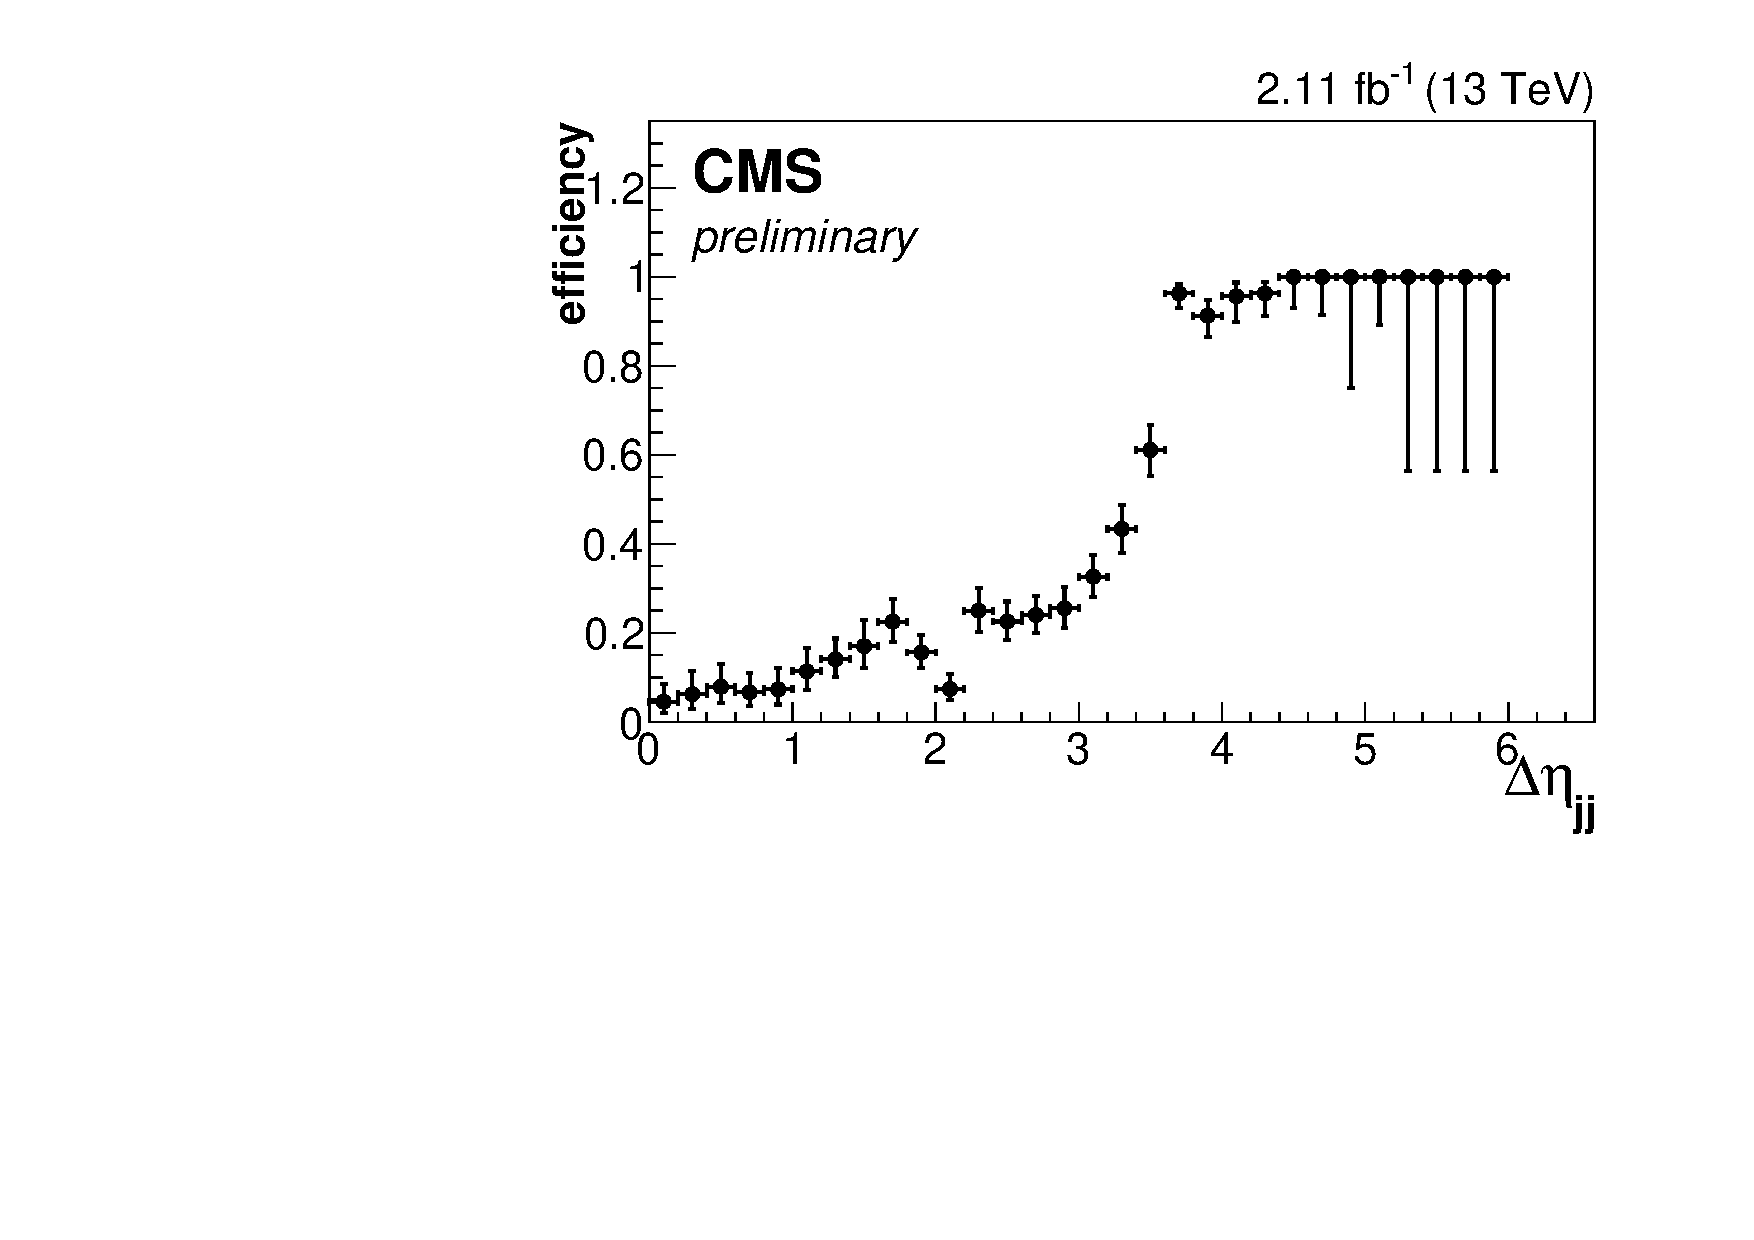
\includegraphics[width=.5\textwidth]{TalkPics/trigeff301115/output_2015Dtrigeff_131115json_sigtrig_301115/nunu_dijet_deta.pdf}
 
\end{frame}

\begin{frame}
  \frametitle{$M_{jj}$ data turn on}
  \scriptsize
  \begin{block}{}
    \begin{itemize}
    \item Measure HLT efficiency (left) and L1+HLT efficiency (right)
    \item Dataset: Full 2015D data with latest JECv6
    \item Trigger: HLT\_DiPFJet40\_DEta3p5\_MJJ600\_PFMETNoMu140
    \item Denominator: SingleMuon events with dijet $p_{T}>80$, $M_{jj}>600$, $\Delta\eta_{jj}>3.6$ plus for left plot only L1ETM60
    \end{itemize}
  \end{block}
  \includegraphics[width=.5\textwidth]{TalkPics/trigeff301115/output_2015Dtrigeff_131115json_sigtrig_hltonly_301115/nunu_dijet_M.pdf}
  \includegraphics[width=.5\textwidth]{TalkPics/trigeff301115/output_2015Dtrigeff_131115json_sigtrig_301115/nunu_dijet_M.pdf}
 
\end{frame}

\begin{frame}  
  \frametitle{Impact of L1MET inefficiencies on signal}
  \scriptsize
  \begin{block}{}
    \begin{itemize}
    \item Check effect of L1 inefficiency as a function of jet eta
    \item MC sample: VBF\_HToInvisible\_M125\_13TeV\_powheg\_pythia8
    \item Denominator: dijet p$_T > 50$ GeV, M$_{jj} > 800$ GeV, $\Delta\eta_{jj} > 3.6$, METnoMU$>200$ GeV\\
    \item L1 inefficiency for jets in the HF can be clearly seen
    \end{itemize}
  \end{block}
  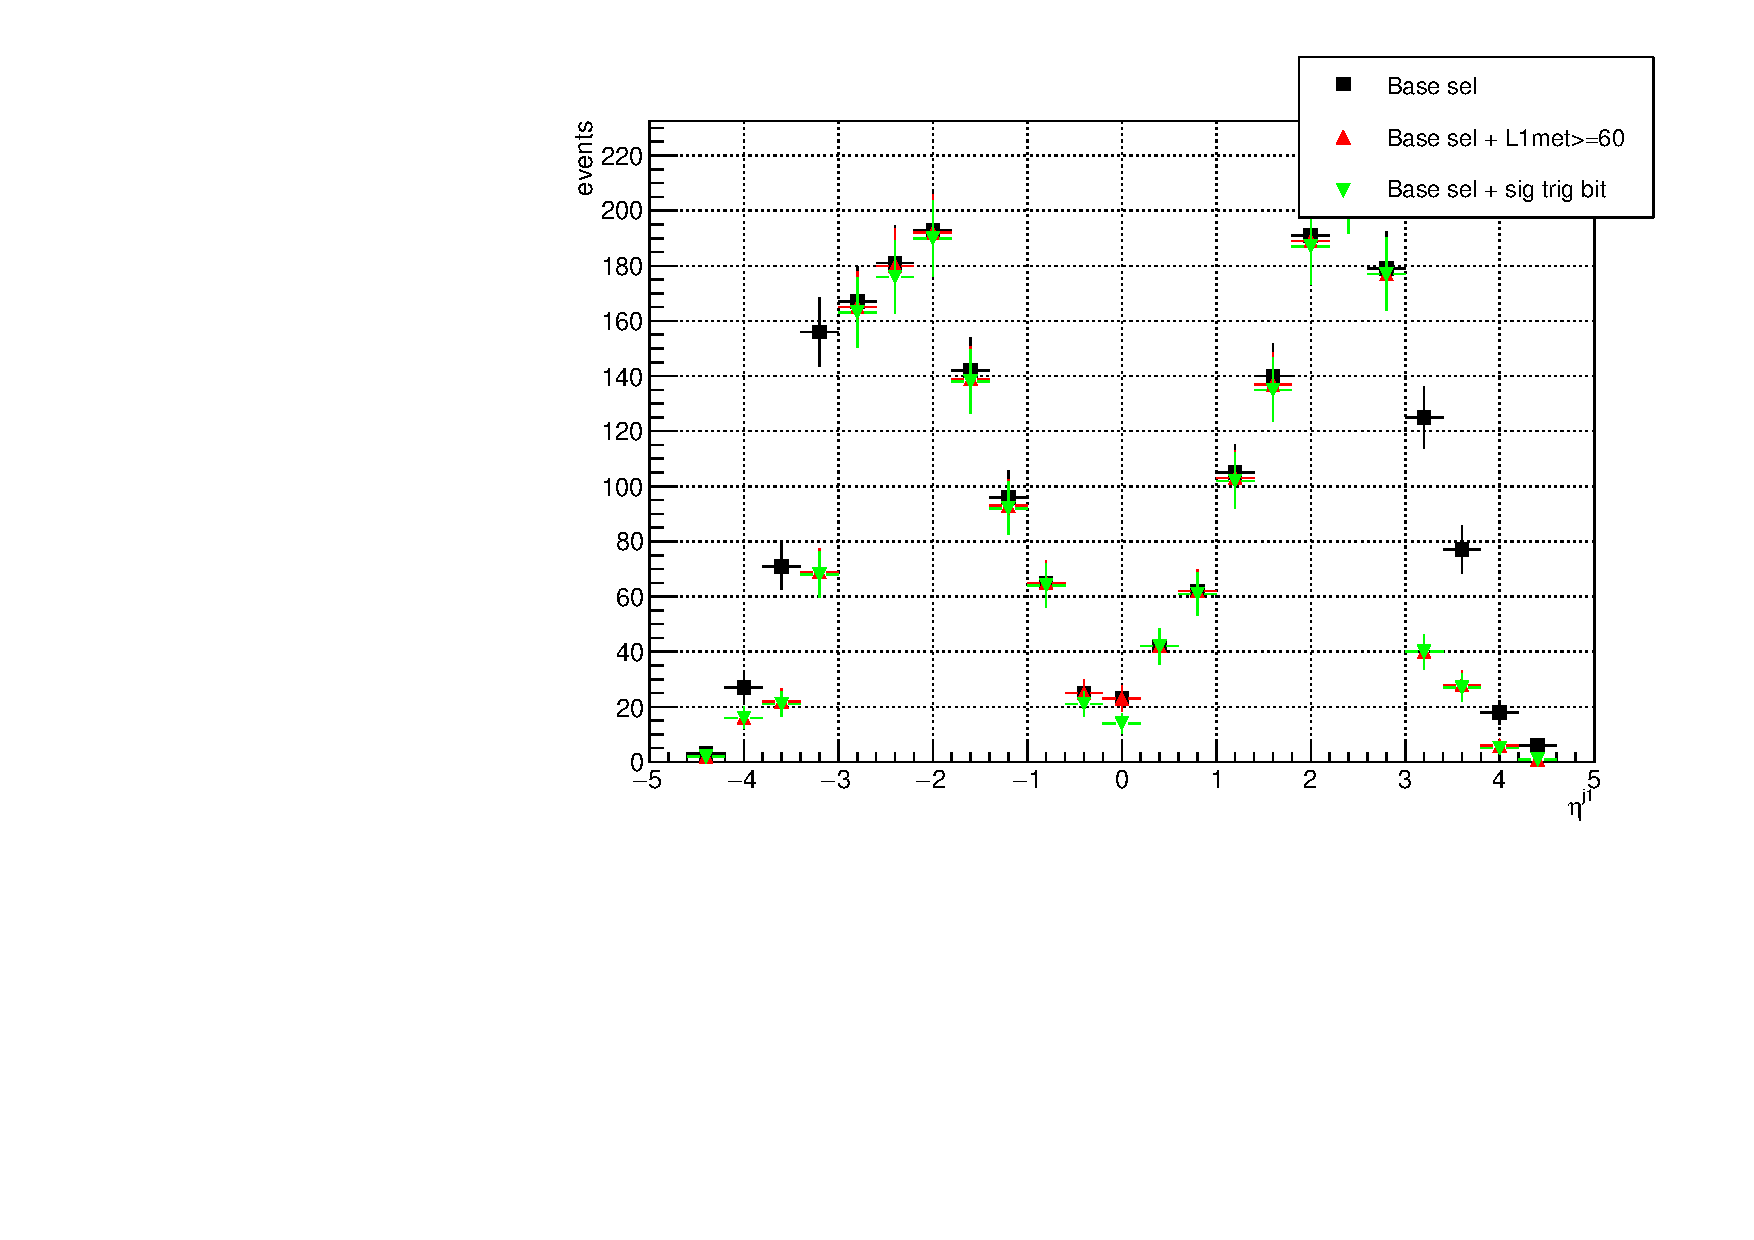
\includegraphics[width=.5\textwidth]{TalkPics/trigeff181115/SigTrigVar_jet1_eta.pdf}
  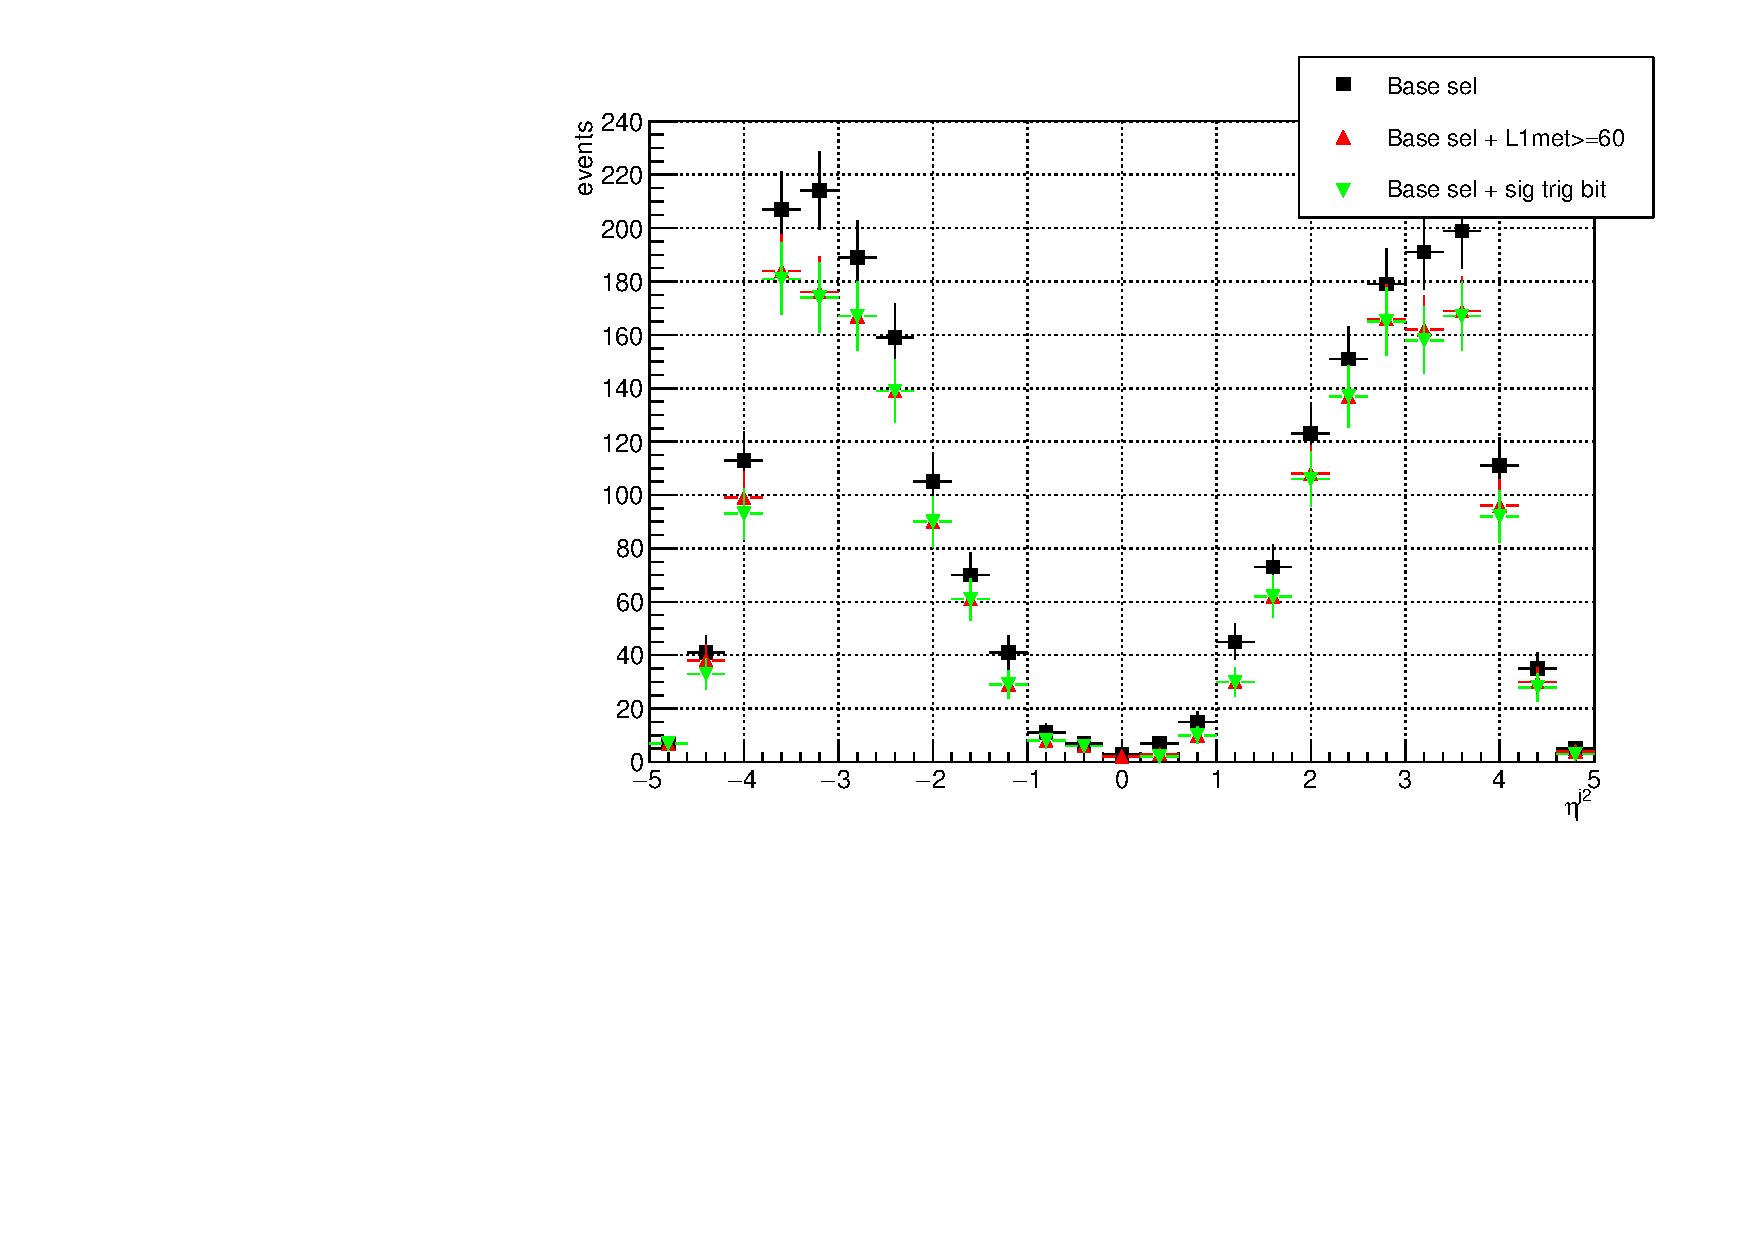
\includegraphics[width=.5\textwidth]{TalkPics/trigeff181115/SigTrigVar_jet2_eta.pdf}
\end{frame}

\begin{frame}  
  \frametitle{Binned trigger efficiencies for first analysis}
  \scriptsize
  \begin{block}{}
    \begin{itemize}
    \item Measure L1+HLT MetNoMu efficiency of signal trigger in bins of jet $p_{T}$ and $M_{jj}$
    \item Dataset: Full 2015D data with latest JECv6
    \item Trigger: HLT\_DiPFJet40\_DEta3p5\_MJJ600\_PFMETNoMu140
    \item Denominator: SingleMuon events with dijet $\Delta\eta_{jj}>3.6$ plus binned cuts
    \item Bins: Jet $p_{T}$: 70-80, 80+, $M_{jj}$: 800-1000, 1000+
    \end{itemize}
  \end{block}
  \begin{columns}
   \column{.5\textwidth}
    Jet $p_{T}$: 70-80, $M_{jj}$: 800-1000
    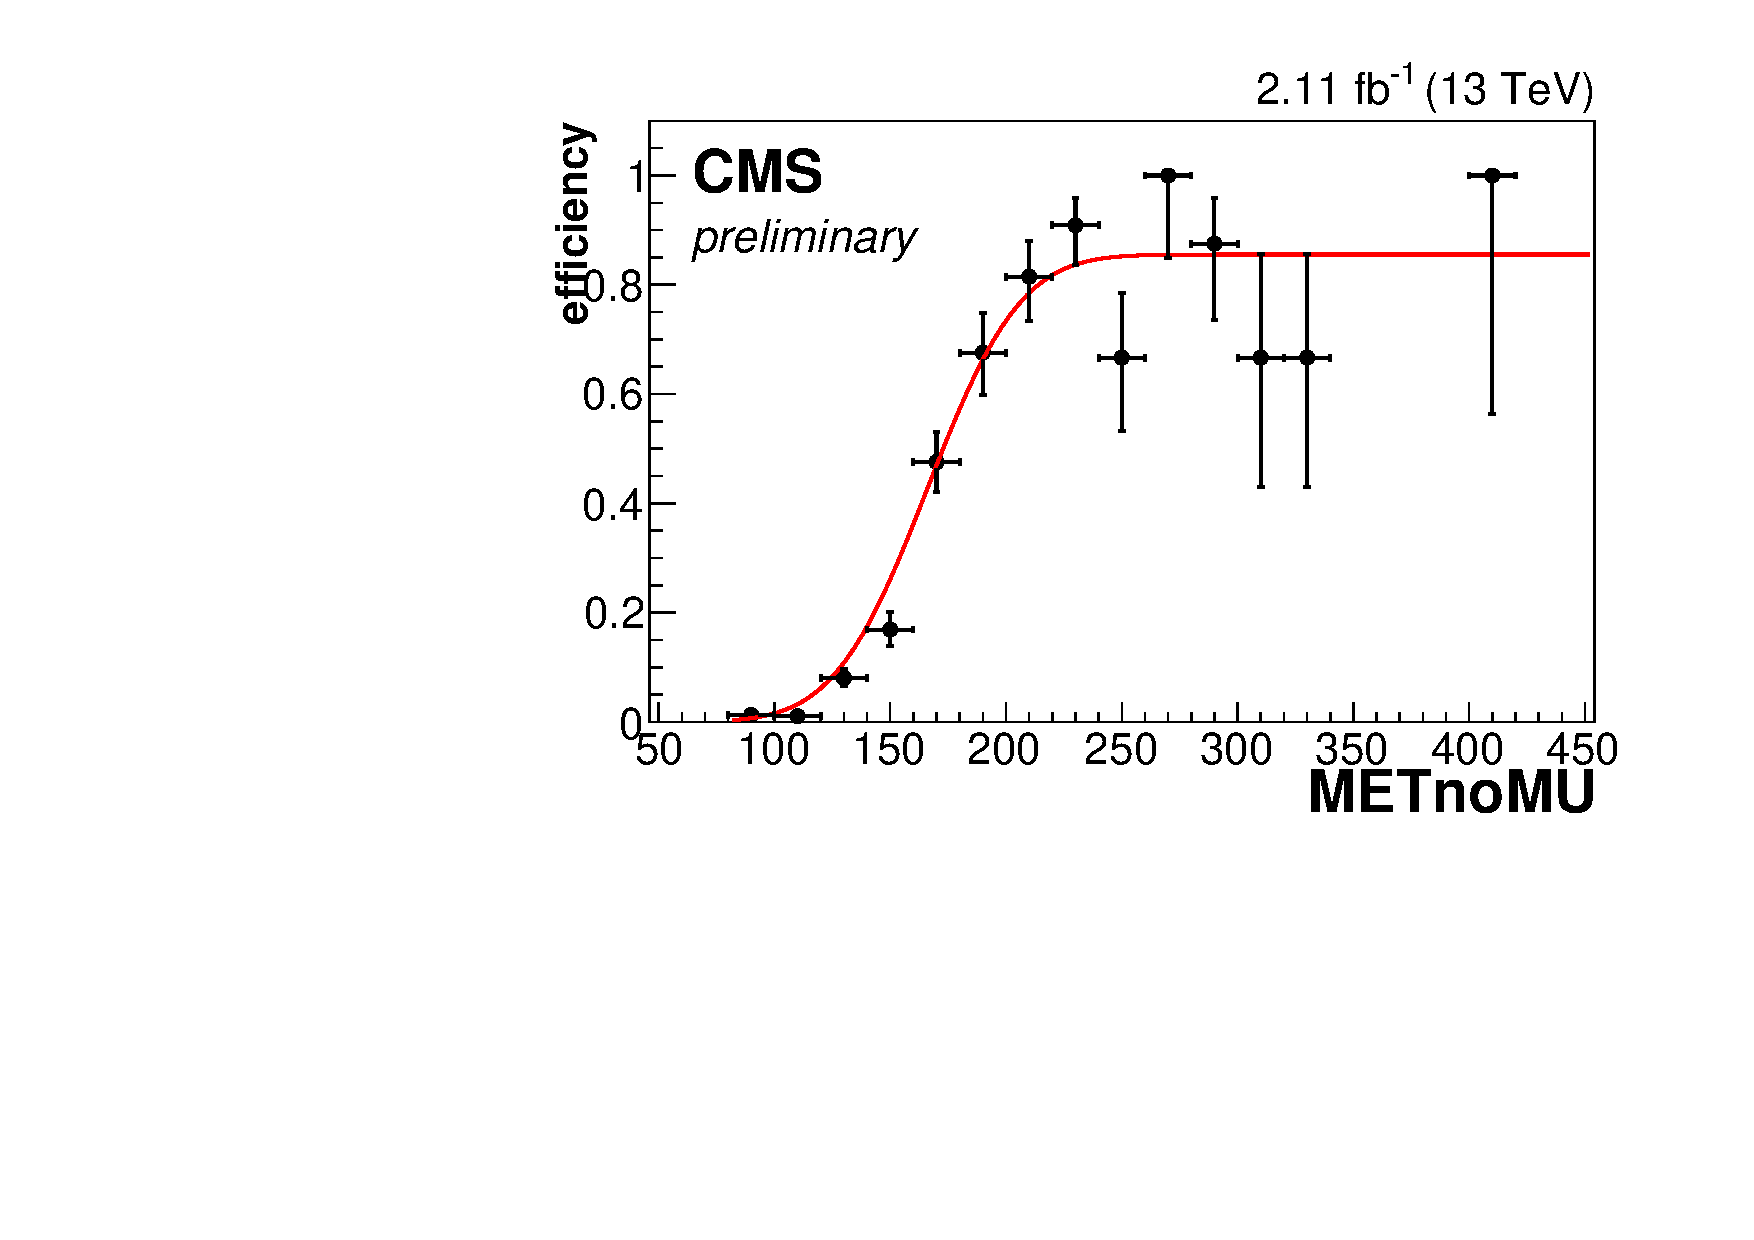
\includegraphics[width=\textwidth]{TalkPics/trigeff261115/output_2015Dtrigeff_131115json_sigtrig_binnedfrom80_241115/nunufdata_MET_1d_11D_metnomuons.pdf}
    \column{.5\textwidth}
    Jet $p_{T}$: 70-80, $M_{jj}$: 1000+
    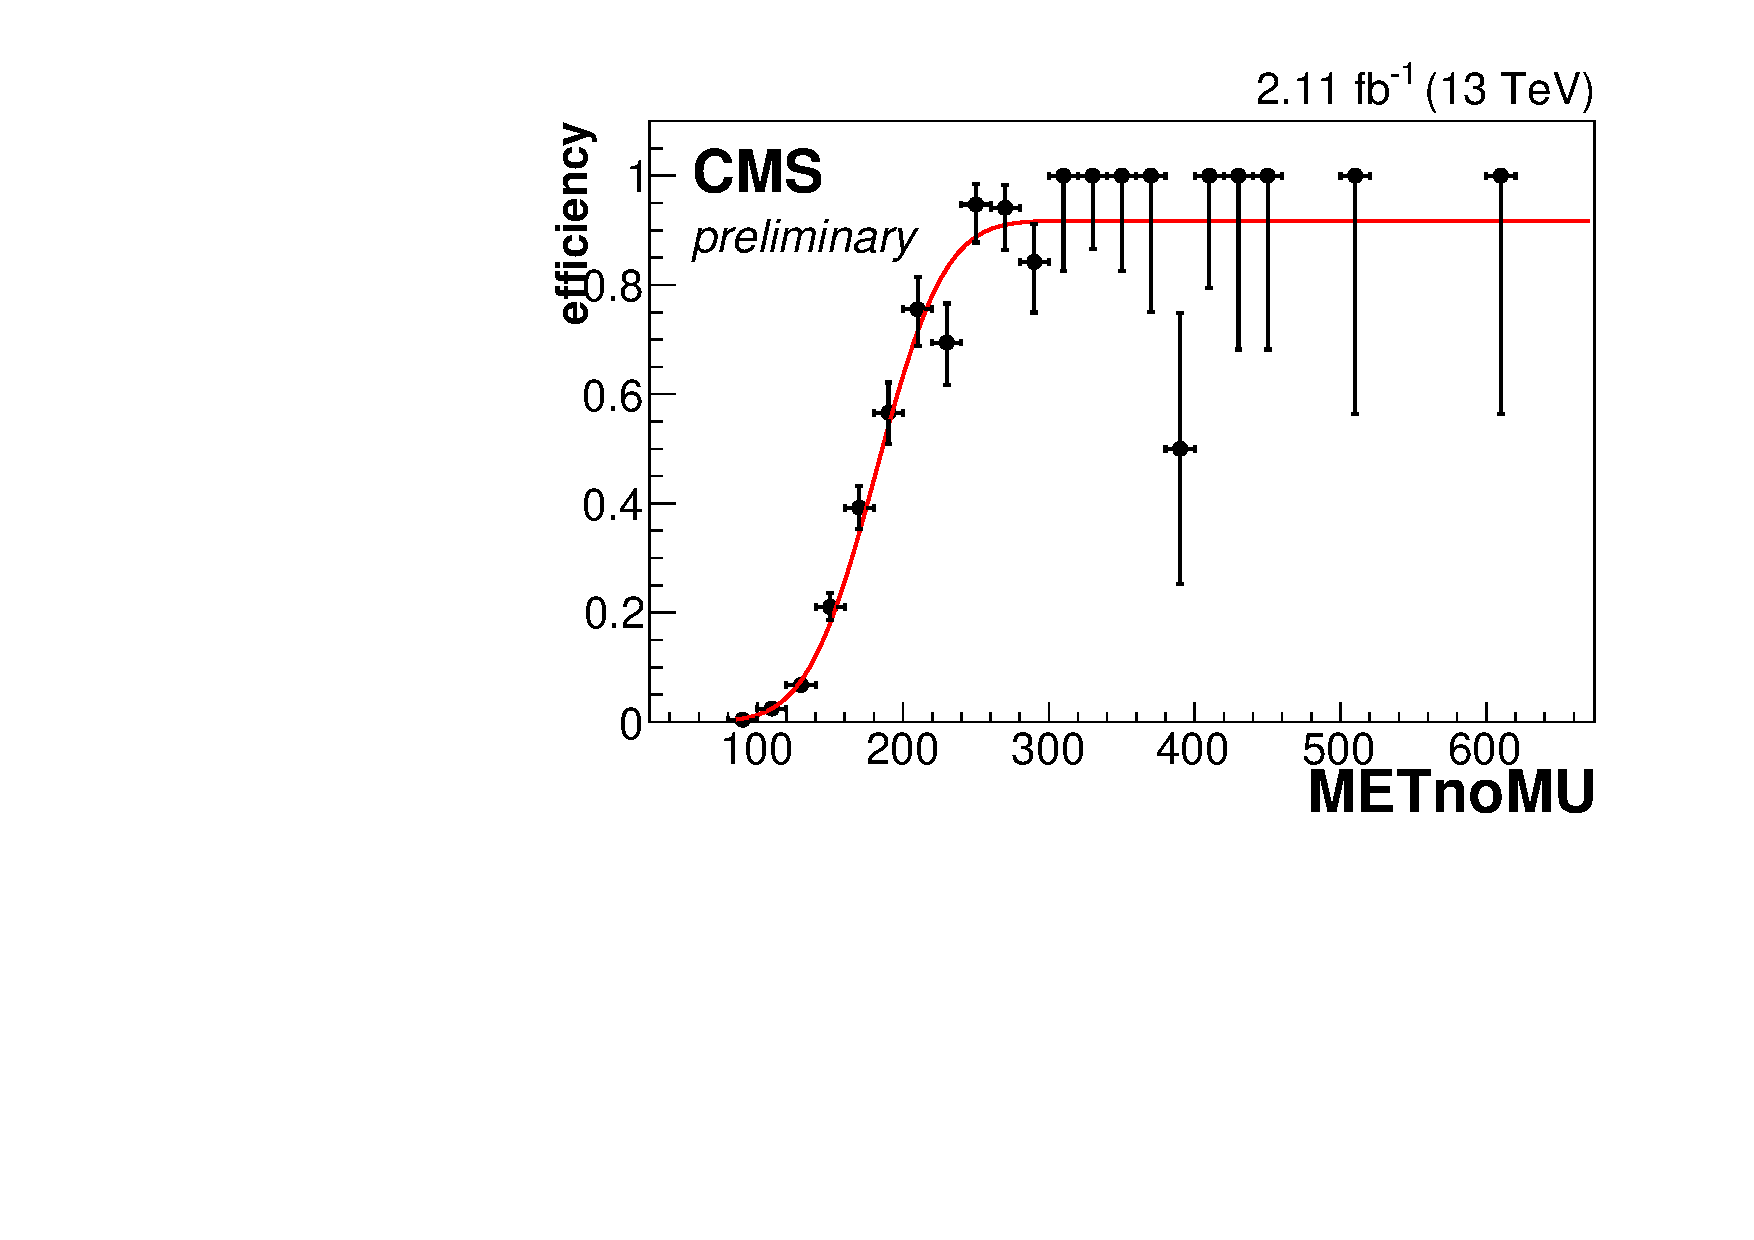
\includegraphics[width=\textwidth]{TalkPics/trigeff261115/output_2015Dtrigeff_131115json_sigtrig_binnedfrom80_241115/nunufdata_MET_1d_12D_metnomuons.pdf}
  \end{columns}
\end{frame}

\begin{frame}  
  \frametitle{Binned trigger efficiencies for first analysis}
  \scriptsize
  \begin{block}{}
    \begin{itemize}
    \item Measure L1+HLT MetNoMu efficiency of signal trigger in bins of jet $p_{T}$ and $M_{jj}$
    \item Dataset: Full 2015D data with latest JECv6
    \item Trigger: HLT\_DiPFJet40\_DEta3p5\_MJJ600\_PFMETNoMu140
    \item Denominator: SingleMuon events with dijet $\Delta\eta_{jj}>3.6$ plus binned cuts
    \item Bins: Jet $p_{T}$: 70-80, 80+, $M_{jj}$: 800-1000, 1000+
    \end{itemize}
  \end{block}
  \begin{columns}
   \column{.5\textwidth}
    Jet $p_{T}$: 80+, $M_{jj}$: 800-1000
    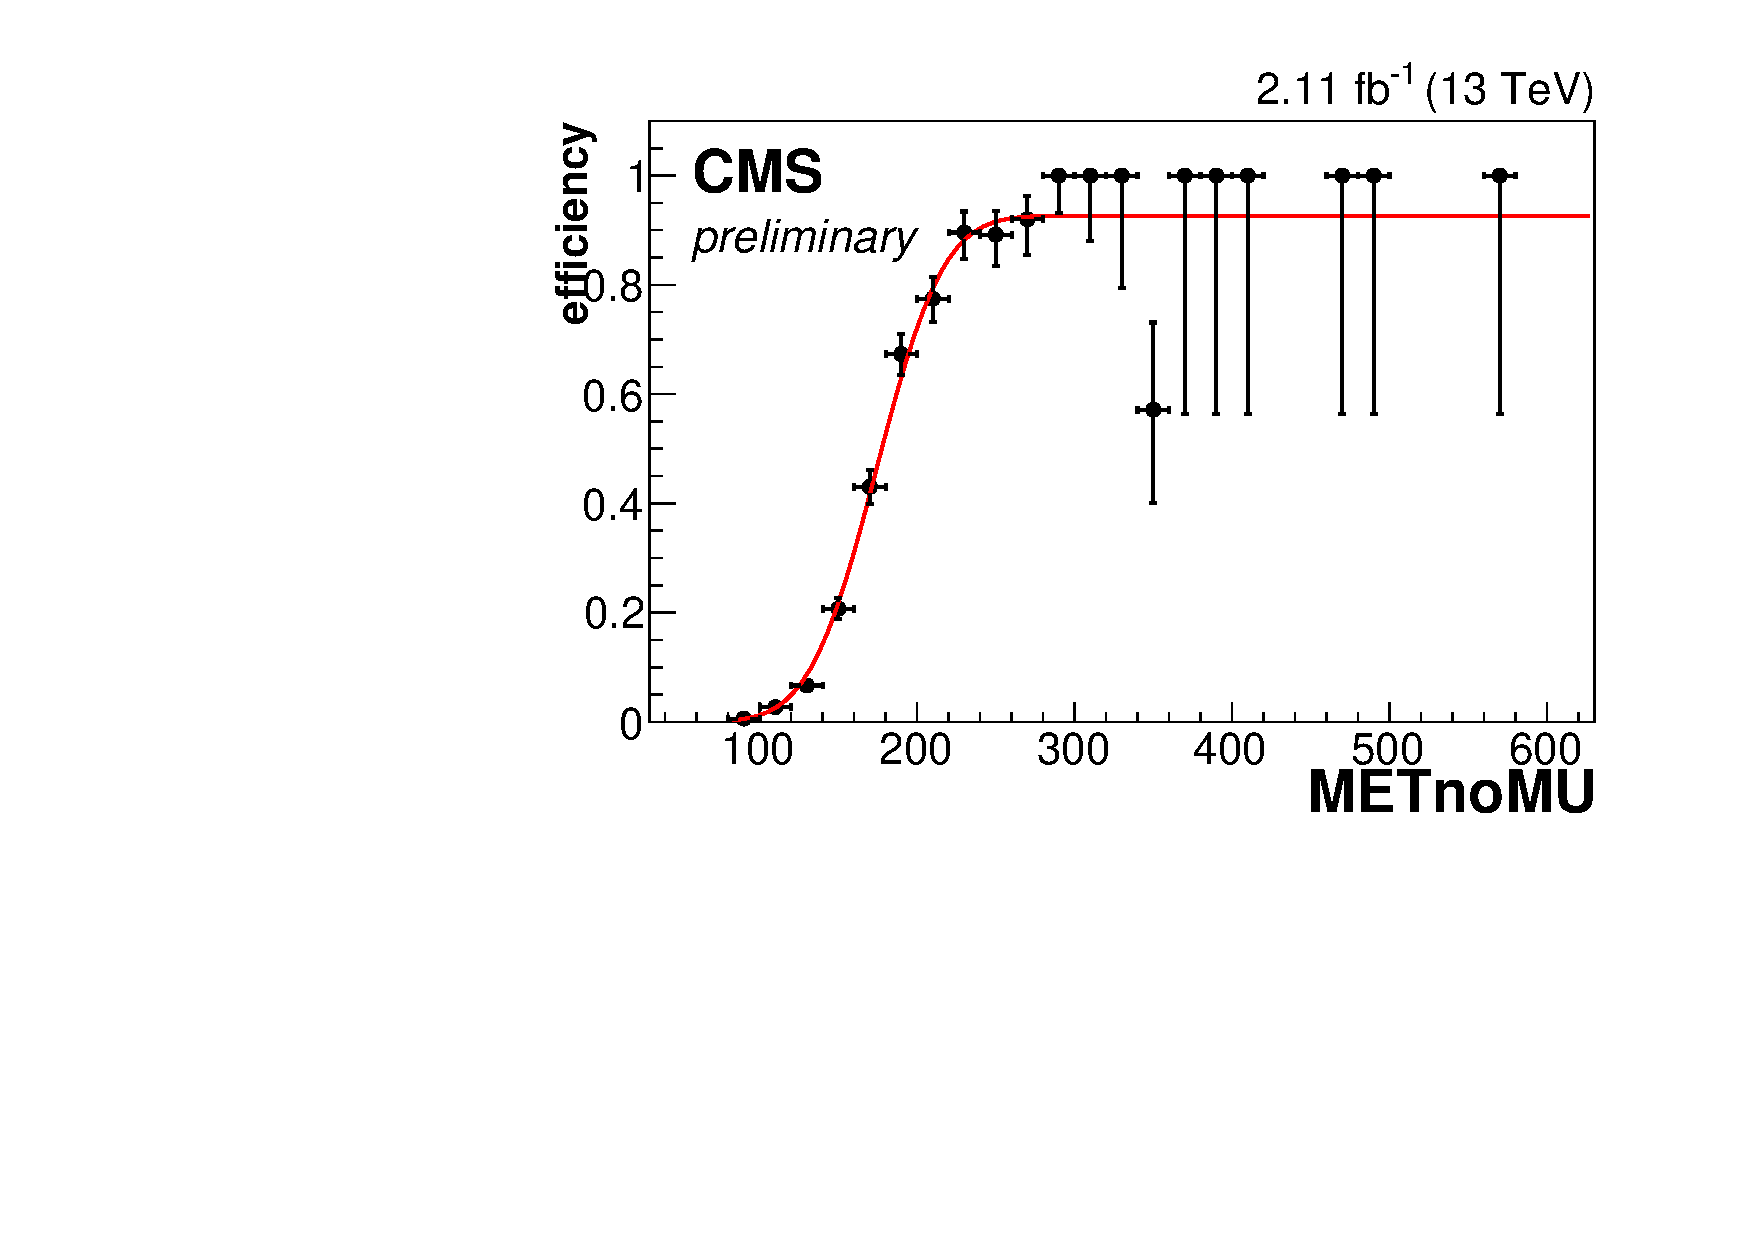
\includegraphics[width=\textwidth]{TalkPics/trigeff261115/output_2015Dtrigeff_131115json_sigtrig_binnedfrom80_241115/nunufdata_MET_1d_21D_metnomuons.pdf}
    \column{.5\textwidth}
    Jet $p_{T}$: 80+, $M_{jj}$: 1000+
    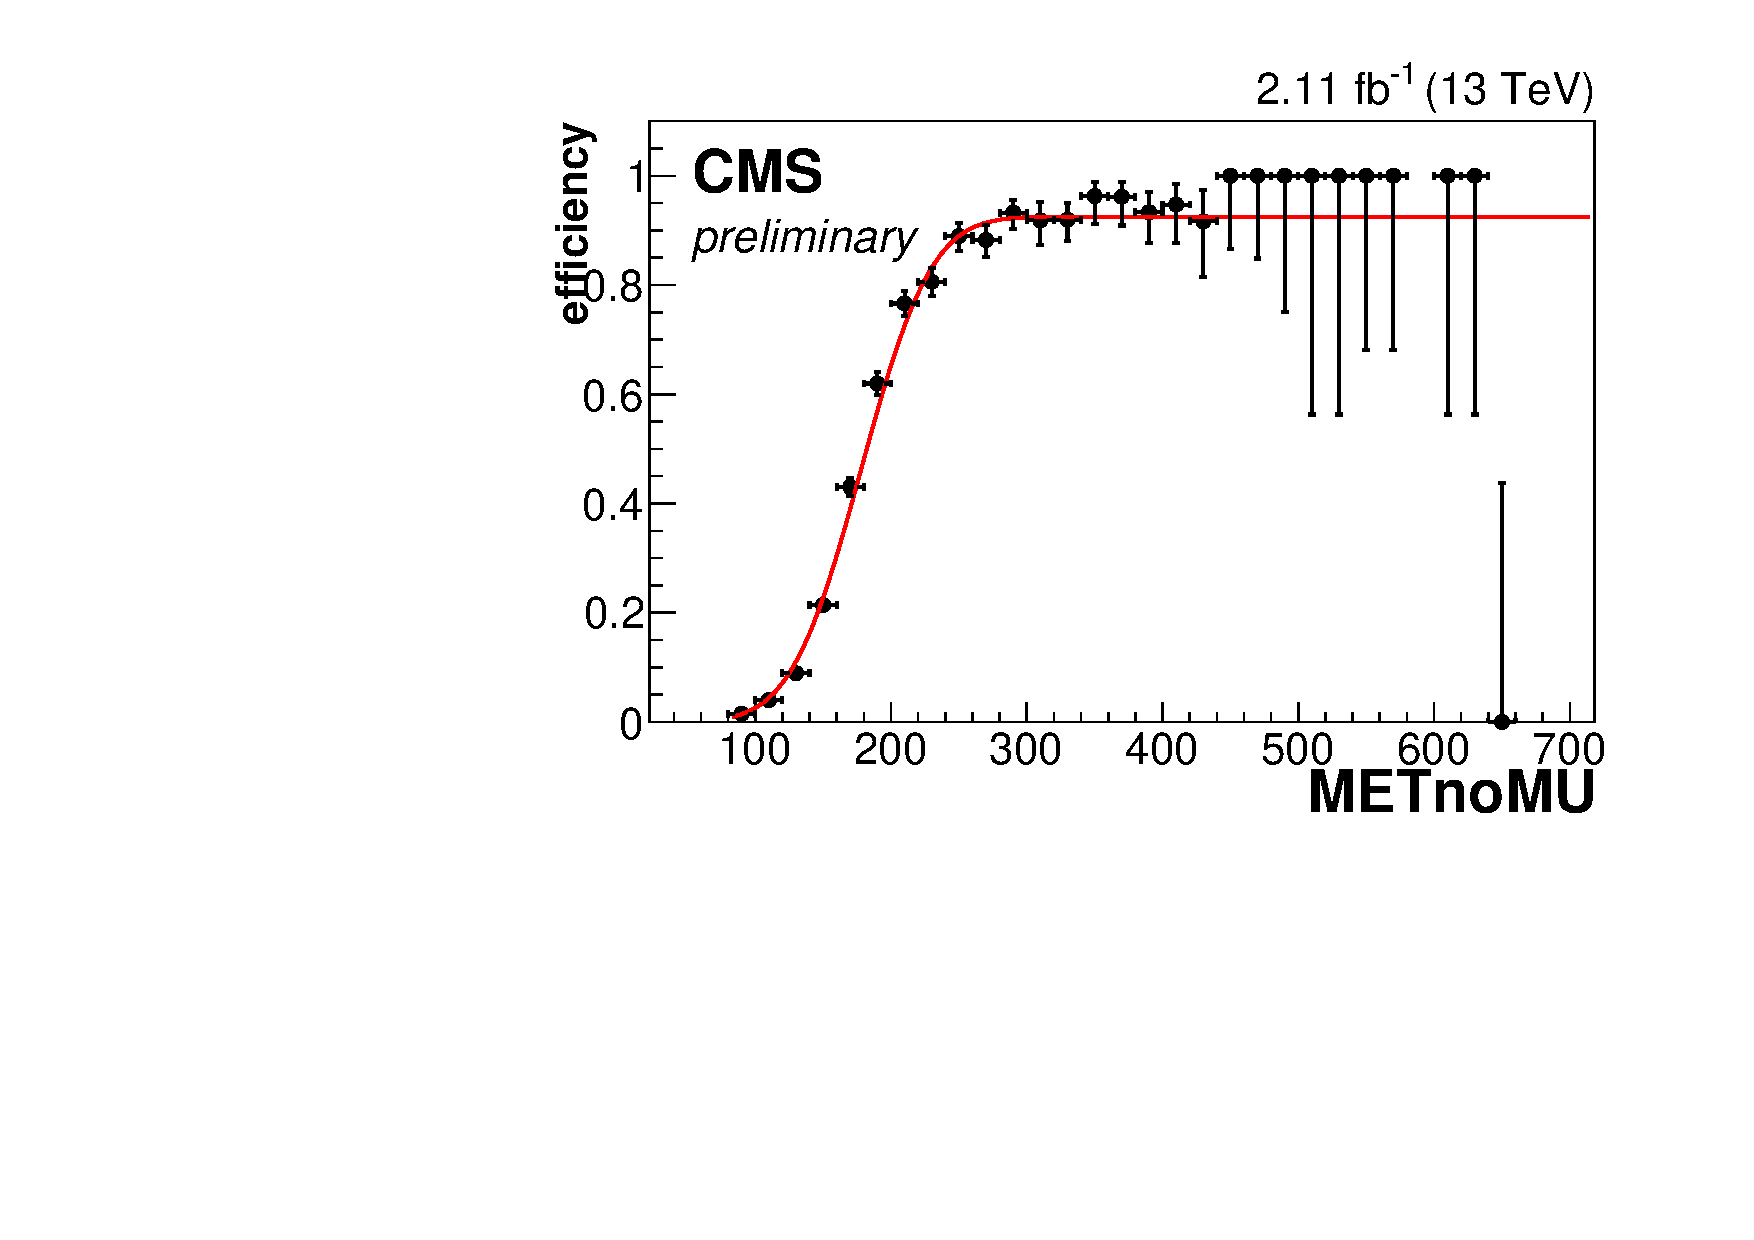
\includegraphics[width=\textwidth]{TalkPics/trigeff261115/output_2015Dtrigeff_131115json_sigtrig_binnedfrom80_241115/nunufdata_MET_1d_22D_metnomuons.pdf}
  \end{columns}
\end{frame}




%  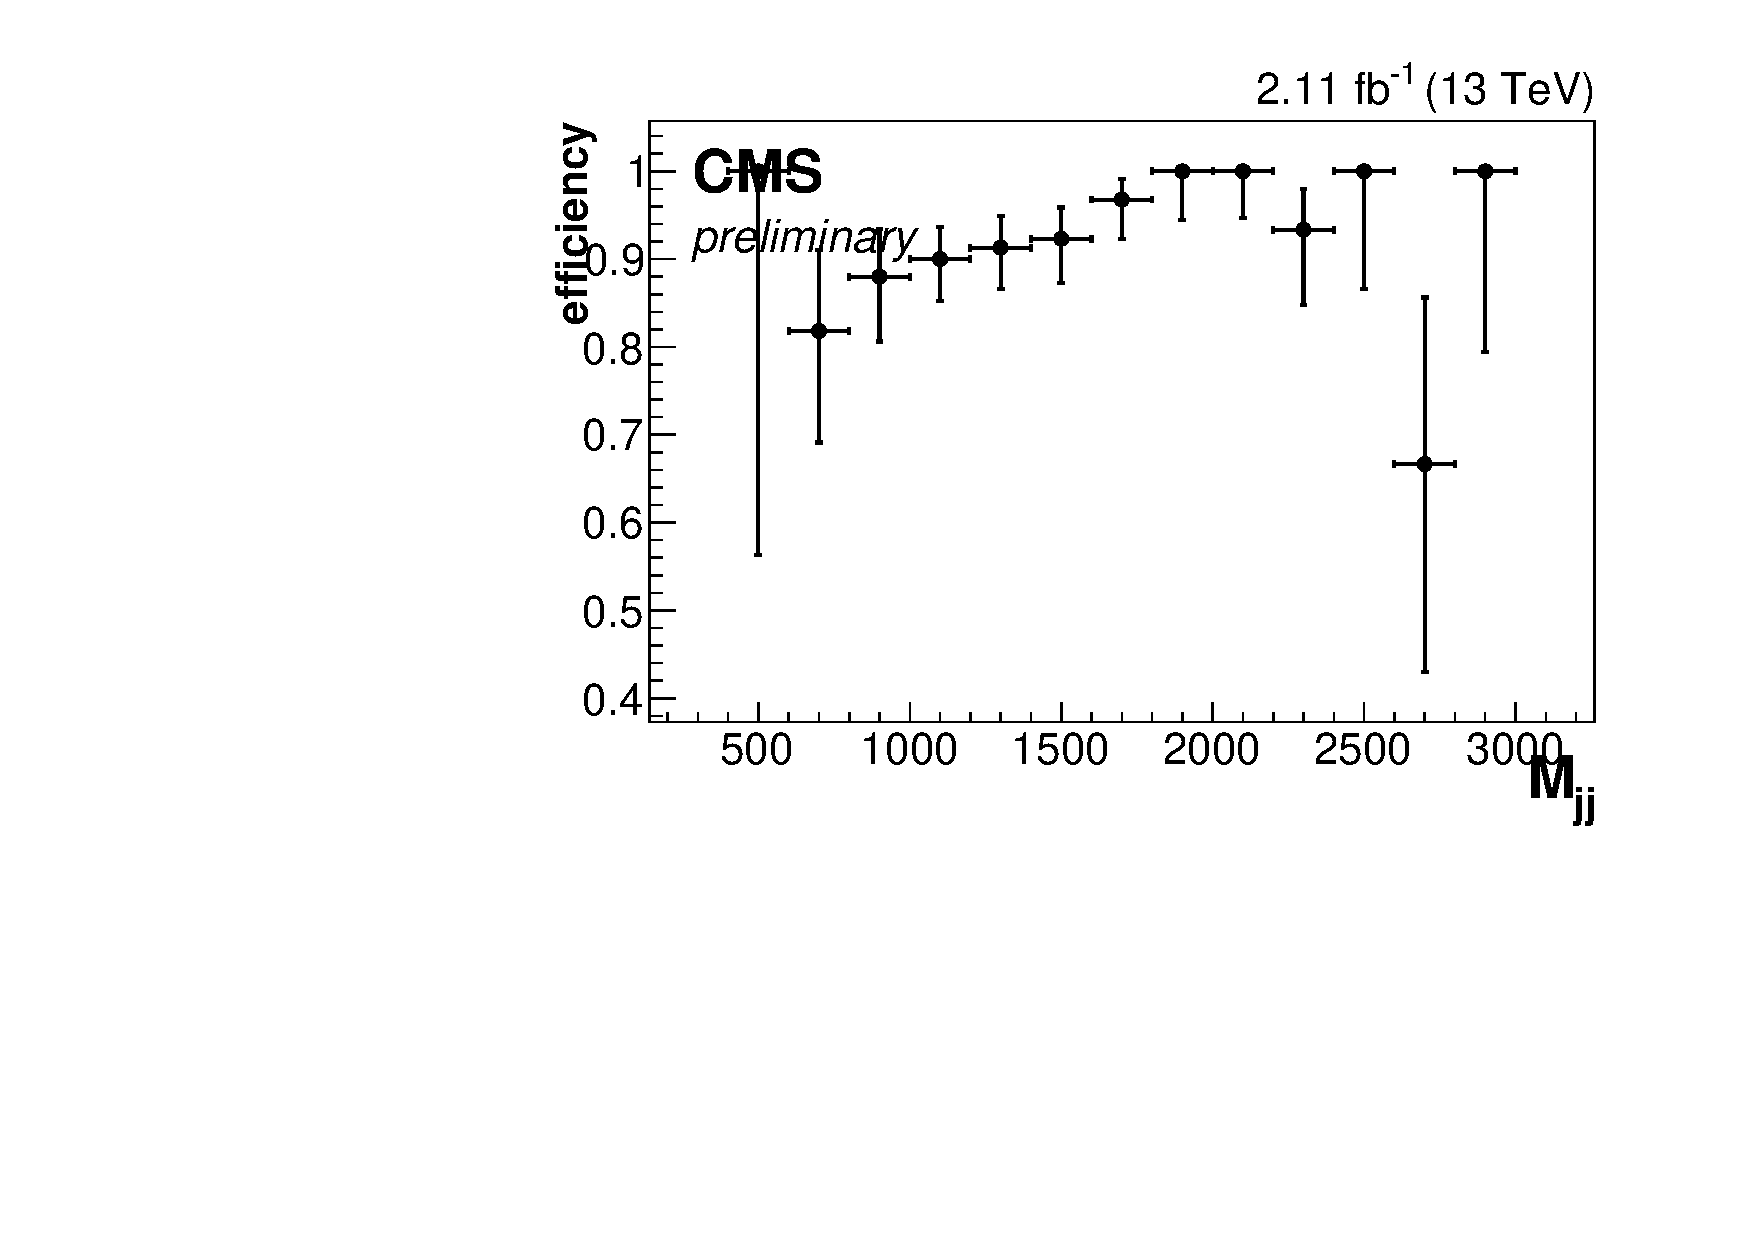
\includegraphics[width=.5\textwidth]{TalkPics/trigeff181115/output_2015Dtrigeff_131115json_sigtrig_met300jpt80_181115/nunu_dijet_M.pdf}
\end{fmffile}
\end{document}
